\documentclass[german,oneside,color]{htldipl}
% Zulässige Class Options: 
%   Hauptsprache: german (default), english
%   Doppelseitig: oneside (default), twoside
%   Syntax-Highlighting: color (default), black

% die folgende Zeile einkommentieren für Arial-Ähnliche Schriftart
%\renewcommand{\familydefault}{\sfdefault}

\graphicspath{{images/}}    % Bilderverzeichnis


\usepackage[paper=a4paper,margin=3cm]{geometry}

\makeindex[title=Index]
\makeindex[name=allgemein, title=Allgemeiner Index]
\makeindex[name=name,title={Autoren Index}]
\makeindex[name=title,columns=1,title={Literatur Index}]
\indexsetup{level=\subsection*, toclevel=subsection, noclearpage}


\makeatletter
\@ifpackageloaded{biblatex_legacy}
  {\DeclareIndexNameFormat{default}{%
     \usebibmacro{index:name}{\index[name]}{#1}{#3}{#5}{#7}}}
  {\DeclareIndexNameFormat{default}{%
     \usebibmacro{index:name}{\index[name]}
       {\namepartfamily}
       {\namepartgiven}
       {\namepartprefix}
       {\namepartsuffix}}}
\makeatother

\DeclareIndexFieldFormat{indextitle}{%
  \usebibmacro{index:title}{\index[title]}{#1}}

\renewbibmacro*{bibindex}{%
  \ifbibindex
    {\indexnames{author}%
     \indexnames{editor}%
     \indexnames{translator}%
     \indexnames{commentator}%
     \indexfield{indextitle}}
    {}}

\makeatletter
\DeclareCiteCommand{\repeatfootcite}[\cbx@wrap]
  {\gdef\cbx@keys{}}
  {\xappto\cbx@keys{\thefield{entrykey},}}
  {}
  {\ifcsundef{cbx@lastin@\cbx@keys @\strfield{postnote}}
     {\csnumgdef{cbx@lastin@\cbx@keys @\strfield{postnote}}{-1}}{}%
   \ifsamepage{\value{instcount}}{\csuse{cbx@lastin@\cbx@keys @\strfield{postnote}}}
     {\footnotemark[\csuse{cbx@lastfn@\cbx@keys @\strfield{postnote}}]}
     {\xappto\cbx@cite{\noexpand\footcite%
        [\thefield{prenote}][\thefield{postnote}]{\cbx@keys}%
        \csnumgdef{cbx@lastfn@\cbx@keys @\strfield{postnote}}{\value{\@mpfn}}%
        \csnumgdef{cbx@lastin@\cbx@keys @\strfield{postnote}}{\value{instcount}}}}}

\newrobustcmd{\cbx@wrap}[1]{#1\cbx@cite\gdef\cbx@cite{}}
\def\cbx@cite{}
\makeatother

\makeglossaries
\loadglsentries{glossary}					%beinhaltet Daten für das Glossar
\addbibresource{literatur.bib}     %beinhaltet Daten für das Literarturverzeichnis

%%%----------------------------------------------------------
\begin{document}
%%%----------------------------------------------------------
%Einstellungen an die eigene Diplomarbeit anpassen
\title{NetShare - Multi-Wan Bonding Prototype}
\abteilung{Maschineningenieurwesen}
%\schwerpunkt{} wenn kein Ausbildungsschwerpunkt vorhanden ist z.B. Informatik
\schwerpunkt{}
\studienort{Wiener Neustadt}
\schule{HTBLuVA Wiener Neustadt}
\schullogo{htl.jpeg}
\abgabejahr{2020/21}
\betreuerA{Dipl. Ing. Sebastian Simon}
\betreuerB{}
\betreuerC{}
\betreuerD{}
%\betreuerD{} leer lassen wenn nicht vorhanden
\schuelerA{Alexander Doubrava}
\evidenzA{5AHIF-?}
\subthemaA{TODO SUBTHEMA}
\schuelerB{Stefan Streimel}
\evidenzB{5AHIF-20}
\subthemaB{Erstellen eines Multi-Wan fähigen Windows Treiber}
\schuelerC{Martin Grafl}
\evidenzC{5AHIF-?}
\subthemaC{TODO SUBTHEMA}
\schuelerD{Manuel Lind}
\evidenzD{5AHIF-?}
\subthemaD{TODO SUBTHEMA}
\schuelerE{}
\evidenzE{}
\subthemaE{}
%\schuelerE{} leer lassen wenn nicht vorhanden
%\evidenzE{}
%\subthemaE{}



%%%----------------------------------------------------------
\frontmatter
\maketitle
\tableofcontents
%%%----------------------------------------------------------

\chapter{Vorwort}

Dies ist \textbf{Version \htldiplDate} der \latex-Dokumentenvorlage für 
die Diplomarbeiten an der HTL Wiener Neustadt, basierend auf der
Vorlage für Abschlussarbeiten an der FH Hagenberg erstellt von Dr.\ Wilhelm
Burger\footnote{\url{http://www.fh-hagenberg.at/staff/burger/diplomarbeit/}}.

Die Verwendung dieser Vorlage ist jedermann freigestellt und an
keinerlei Erwähnung gebunden. Allerdings -- wer sie als Grundlage
seiner eigenen Arbeit verwenden möchte, sollte nicht einfach
("`ung'schaut"') darauf los werken, sondern zumindest die
wichtigsten Teile des Dokuments \emph{lesen} und nach Möglichkeit
auch beherzigen. Die Erfahrung zeigt, dass dies die Qualität der
Ergebnisse deutlich zu steigern vermag.

Der Quelltext zu diesem Dokument sowie das zugehörige
\latex-Paket sind in der jeweils aktuellen Version online
verfügbar unter
%
\begin{quote}
\url{https://github.com/wschermann/Diplomarbeitsvorlage}
\end{quote}
%
Trotz großer Mühe enthält dieses Dokument zweifellos Fehler und Unzulänglichkeiten
-- Kommentare, Verbesserungsvorschläge und passende Ergänzungen
sind daher stets willkommen, am einfachsten per E-Mail direkt an mich:
\begin{center}%
\begin{tabular}{l}
\nolinkurl{w.schermann@htlwrn.ac.at} \\
Wolfgang Schermann MSc \\
HTL Wiener Neustadt -- Informatik\\
Austria
\end{tabular}
\end{center}

\noindent
Übrigens, hier im Vorwort kann man kurz auf die Entstehung  des Dokuments eingehen.
Hier ist auch der Platz für allfällige Danksagungen (\zB an den Betreuer, 
den Begutachter, die Familie, den Hund, ...), Widmungen und philosophische 
Anmerkungen. Das sollte man allerdings auch nicht übertreiben und sich auf 
einen Umfang von maximal zwei Seiten beschränken.




				%ggfs. weglassen
%Inkludiert die 4. vorgeschriebenen Seiten an Dokumentation aus dem gedruckten PDF-Formular
%Das Formular erst vor der Abgabe vollständig ausfüllen, da z.B. das Bild zur Diplomarbeit vorher nicht vorhanden sein wird
\begingroup
\makeatletter
\newpage
\@twosidefalse
\includepdf[pages=1-1,pagecommand={\chapter[Diplomarbeit Dokumentation]{}}]{pdf/Formular-printed.pdf}
\includepdf[pages=2-2,pagecommand={\thispagestyle{plain}}]{pdf/Formular-printed.pdf}
\includepdf[pages=3-3,pagecommand={\chapter[Diploma Thesis Documentation]{}}]{pdf/Formular-printed.pdf}
\includepdf[pages=4-4,pagecommand={\thispagestyle{plain}}]{pdf/Formular-printed.pdf}
\endgroup
\chapter{Kurzfassung}

An dieser Stelle steht eine Zusammenfassung der Arbeit, Umfang
max.\ 1 Seite. Im Unterschied zu anderen Kapiteln ist die
Kurzfassung (und das Abstract) üblicherweise nicht in Abschnitte
und Unterabschnitte gegliedert. 
Auch Fußnoten sind hier falsch am Platz.

Kurzfassungen werden übrigens häufig -- zusammen mit Autor und Titel
der Arbeit -- %
in Literaturdatenbanken aufgenommen. Es ist daher darauf zu
achten, dass die Information in der Kurzfassung für sich 
\emph{allein} (\dah ohne weitere Teile der Arbeit) zusammenhängend und
abgeschlossen ist. Insbesondere werden an dieser Stelle (wie \ua
auch im \emph{Titel} der Arbeit und im \emph{Abstract})
normalerweise \emph{keine Literaturverweise} verwendet! Falls man
unbedingt solche benötigt -- etwa weil die Arbeit eine
Weiterentwicklung einer bestimmten, früheren Arbeit darstellt --,
dann sind \emph{vollständige} Quellenangaben in der Kurzfassung
selbst notwendig, \zB %
[\textsc{Zobel} J.: \textit{Writing for Computer Science -- The Art of
Effective Commu\-nica\-tion}. Springer-Verlag, Singa\-pur, 1997].

Weiters sollte man daran denken, dass bei der Aufnahme in Datenbanken
Sonderzeichen oder etwa Aufzählungen mit "`Knödellisten"' in der
Regel verloren gehen. Dasselbe gilt natürlich auch für das 
\emph{Abstract}.


Inhaltlich sollte die Kurzfassung \emph{keine} Auflistung der
einzelnen Kapitel sein (dafür ist das Einleitungskapitel
vorgesehen), sondern dem Leser einen kompakten, inhaltlichen
Überblick über die gesamte Arbeit verschaffen. Der hier verwendete
Aufbau ist daher zwangsläufig anders als der in der Einleitung.
		
\chapter{Abstract}

\begin{english} 
    This diploma thesis deals with the planning and development of a multi-wan bonding prototype, called NetShare. As  Windows does not offer a free-of-charge option to use several internet connections simultaneously and to bundle their bandwidths, we decided to develop such a prototype. 
    \\\\
    For the implementation we need a multi-wan bonding capable server, driver and a Windows desktop application to control the driver. For this reason, we have dealt with the following technologies IP Routing Table, Nating, TUN-/ TAP devices, Virtual Private Networks, Winforms, and Windows drivers.
    \\\\
    In the thesis, we explain the technologies used and the approaches followed in the implementation of our multi-wan bonding prototype. Furthermore, we illustrate with the help of examples how the individual functions have been implemented. 
\end{english}
			

%%%----------------------------------------------------------
\mainmatter           %Hauptteil (ab hier arab. Seitenzahlen)
%%%----------------------------------------------------------

\chapter{Einleitung}
\label{cha:Einleitung}

\section{Projekthintergrund und Idee}
In einer Zeit der rasant voranschreitenden Digitalisierung, ist eine schnelle Internetverbindung zur Voraussetzung des täglichen Alltags geworden. Aufgrund von oft mangelhafter Infrastruktur, haben wir uns dazu entschieden einen Multi-Wan Bonding Prototyp zu entwickeln, welcher die Bündelung mehrere Internetverbindungen ermöglicht. Dadurch könnte eine schnelle und stabiler Internetanbindung erreicht werden. Es soll für den Anwender mithilfe einer simplen Desktop-Anwendung möglich sein, mehrere Internetverbindungen auszuwählen und diese gebündelt nutzen zu können.
\section{Gliederung der Diplomschrift}
\paragraph{Kapitel 2 Technologien für Multi-Wan Bonding}erläutert die verwendeten Technologien die uns bei der Implementierung des Prototypen in hinsicht auf Multi-Wan Bonding geholfen haben.
\paragraph{Kapitel 3 Technologien für Windows Desktop-Anwendungen}beschreibt die Technologien die wir zum Erstellen der Windows Desktop-Anwendung verwendet haben.
\paragraph{Kapitel 4 Verwandte Arbeiten}listet andere Lösungen im Bereich Multi-Wan Bonding auf. 
\paragraph{Kapitel 5...}
\paragraph{Kapitel 6 Multi-Wan Bonding Treiber für Windows}veranschaulicht sowohl die Herangehensweise der Implementierung, als auch die Architektur des Multi-Wan Bonding Treibers.
\paragraph{Kapitel 7 Windows Desktop-Anwendung zur Steuerung des Treibers}beschreibt die Implementierung des Designs und der Funktionalität der Desktop-Anwendung, sowie die Kommunikation mit dem Multi-Wan Bonding Treiber.
\paragraph{Kapitel 8 Funktionstests für Multi-Wan Bonding}gibt den Testaufbau und die Testergebnisse bei unseren Integrationstests wieder.
\chapter{Zum Arbeiten mit \latex}
\label{cha:ArbeitenMitLatex}



\section{Start}
\label{sec:latex}



\latex ist eine in den Naturwissenschaften sehr verbreitete
und mittlerweile klassische Textverarbeitungssoftware für das Erstellen
großer und komplizierter Dokumente mit professionellem Anspruch.
Das Arbeiten mit \latex erscheint -- zumindest für den ungeübten Benutzer -- %
zunächst schwieriger als mit herkömmlichen Werkzeugen für die
Textverarbeitung.

Zum Ersten ist -- im Unterschied zu den meisten gängigen
Text\-ver\-arbei\-tungs\-prog\-ram\-men -- \latex nicht \textsc{Wysiwyg}%
\footnote{"`What You See Is What You Get."' Es gibt auch 
\textsc{Wysiwyg}-Implementierungen für \latex, 
\zB\ \emph{Scientific WorkPlace} (\url{http://www.mackichan.com}) oder
\emph{LyX} (\url{http://www.lyx.org}), 
die aber teuer \bzw\ relativ langsam sind.},
sondern es handelt sich um eine \emph{Markup Lang\-uage} (wie HTML) -- noch dazu
eine recht komplizierte -- und zugehörige Werkzeuge.
Ungewohnt erscheinen sicher auch die vermeintlich starken
Einschränkungen von \latex,
insbesondere in Bezug auf die Wahl der Schriften und das
Layout. Während man anfangs meint, dass diese Rigidität
die eigene Kreativität beschränkt, bemerkt man mit der Zeit, dass es gerade
dadurch gelingt, sich stärker auf die Inhalte der Arbeit zu
konzentrieren als auf deren äußere Form. Dass am Ende die Form dennoch stimmt,
ist allerdings nur dann gewährleistet, wenn man sich bei den eigenen Modifikationen
der Formate und Parameter äußerste Zurückhaltung auferlegt, es sei denn,
man ist in der Zwischenzeit bereits selbst zum \latex-\emph{Guru} avanciert.

Insgesamt lohnt sich der Aufwand, wie viele meinen, zumal die Diplomarbeit
in jedem Fall (mit oder ohne \latex) ein substantielles Stück Arbeit ist.
Es sollte mithilfe von \latex ein professionell aussehendes
Ergebnis einfacher zu erreichen sein und man wird sich wohl auch einigen
Ärger mit Bugs und Unzulänglichkeiten gängiger Software ersparen.
Zudem könnte es durchaus sein, dass man nebenbei auch sein Auge für
die Feinheiten des Buchsatzes (weiter-) entwickelt.

\subsection{Software}

Zum Arbeiten mit \latex benötigt man -- neben einem Computer -- natürlich Software. Musste man sich früher oft die einzelnen Komponenten von \latex mühevoll zusammensuchen und für die eigene Umgebung konfigurieren, gibt es mittlerweile für die wichtigsten Plattformen (Windows, Mac~Os, Linux) fertige \latex-Installationen, die ohne weiteres Zutun laufen. Die aktuelle Version von \latex\ ist \LaTeXe\ (sprich "`LaTeX zwei e"'). 
Zum Arbeiten mit \latex\ benötigt man zwei Dinge:
%
\begin{itemize}
\item \latex-Installation (Distribution)
\item Texteditor oder Autorenumgebung (Frontend)
\item PDF-Software 
\end{itemize}
%
Sämtliche Komponenten sind kostenlos und für alle gängigen Plattformen verfügbar.

Die Distribution beinhaltet mehrere ausführbare Dateien die zusammen aus dem Dokument das PDF erstellen. Je nach verwendeter Software müssen die Einstellungen für diese Programme eventuell manuell angepasst werden.

Die für die Vorlage notwendigen Programme sind:
\begin{itemize}
	\item \textbf{pdflatex} erstellt die PDF Datei (z.B. unter Windows pdflatex.exe) mit den Argumenten \textit{-interaction=nonstopmode "\%wm" }
	\item \textbf{biber} erstellt das Literatur-Verzeichnis (z.B. unter Windows biber.exe) mit den Argumenten \textit{"\%wm" }
	\item \textbf{makeindex} erstellt das Inhaltsverzeichnis und die Nummerierung der Kapitel,... (z.B. unter Windows makeindex.exe) mit den Argumenten \textit{"\%tm.idx" -t "\%tm.ilg" -o "\%tm.ind" }
	\item \textbf{makeglossaries} erstellt die Glossaren (z.B. unter Windows makeglossaries-lite.exe) mit den Argumenten \textit{-s "\%tm.ist" -t "\%tm.glg" -o "\%tm.gls" "\%tm.glo" }
\end{itemize}

\subsubsection{Windows}

Unter \gls{Windows}\index[allgemein]{Windows} (7, 8, 10) hat sich folgendes Setup bewährt,
mit dem \ua auch dieses Dokument erstellt wurde:
%
\begin{itemize}
\item \textbf{\latex-Distribution}: \emph{MikTeX 2.9} oder höher.
MikTeX enthält auch alle notwendigen Hilfsprogramme, wie beispielsweise {\tt biber}.%
\footnote{\url{http://www.miktex.org}}
\item \textbf{Frontend}: \emph{TeXnicCenter}.%
\footnote{\url{http://www.texniccenter.org}}
Grundsätzlich kann man jeden Text-Editor%
\footnote{Unter Windows \zB\ \emph{Ultra\-Edit} (\url{http://www.ultraedit.com})
oder \emph{WinEdit} (\url{http://www.winedit.com}).} verwenden, praktischer ist jedoch eine integrierte \latex-Umgebung wie TeXnicCenter, die einen auch bei 
der Dateiverwaltung, der Verarbeitung der Dokumente und der Fehlerbehandlung unterstützt. Für diese Vorlage wird mindestens die Version 2.0 benötigt, da sonst keine Unicode Unterstützung gegeben ist.\footnote{\url{http://www.texniccenter.org}}
\item \textbf{PDF-Viewer}: \emph{Adobe Acrobat Reader}%
\footnote{\url{https://get.adobe.com/de/reader/}}
\end{itemize}
Beim erstem Mal sollten \emph{MikTeX} und \emph{TeXnicCenter} in genau dieser Reihenfolge installiert werden.

MikTeX sollte so eingerichtet werden, dass fehlende Pakete automatisch geladen werden. Beim ersten Erstellen der Arbeit werden dann alle notwendigen Pakete aus dem Internet geladen und stehen ab dann lokal zur Verfügung. Das erste Erstellen dauert dadurch allerdings mitunter sehr lange. Sollten trotzdem noch fehlende Pakete wie \zB\ \emph{tracklang.sty} angezeigt werden, so muss noch MikTeX aktualisiert werden. Update (Admin) im Startmenü von MikTeX unter Maintenance. Das Programm wählt automatisch die richtigen Pakete zur Aktualisierung aus. Sollten dann immer noch Pakete fehlen, sollte auch noch die Datenbank von MikTeX aktualisiert werden (Im MikTeX Pakete-Manager).

Bei der Diplomarbeitsvorlage ist mit \texttt{\_Diplomarbeitsvorlage.tcp} bereits ein vorgefertigtes TeXnicCenter-Projekt enthalten. Damit dieses Projekt vollständig kompiliert werden kann, muss im TeXnicCenter noch das Ausgabeprofil korrekt eingestellt werden. Dieses Ausgabeprofil kann aus der Datei \texttt{\_Ausgabeprofil.tco} importiert werden oder gemäß der Abbildung \ref{fig:Settings} eingestellt werden. Die nicht vollständig sichtbaren Argumente bei \texttt{makeglossaries} sind \verb|-s "%tm.ist" -t "%tm.glg" -o "%tm.gls" "%tm.glo"|.

\begin{figure}
    \centering
    \begin{subfigure}[t]{0.45\textwidth}
        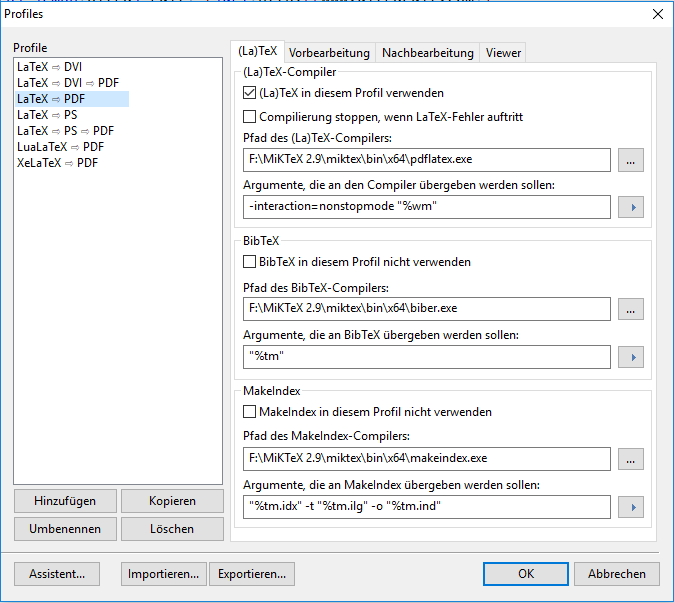
\includegraphics[width=\linewidth]{TeXnicCenterEinstellungen.PNG}
    \caption{Einstellungen für pdflatex, biber und makeindex}
		\end{subfigure}\hfill
    \begin{subfigure}[t]{0.45\textwidth}
        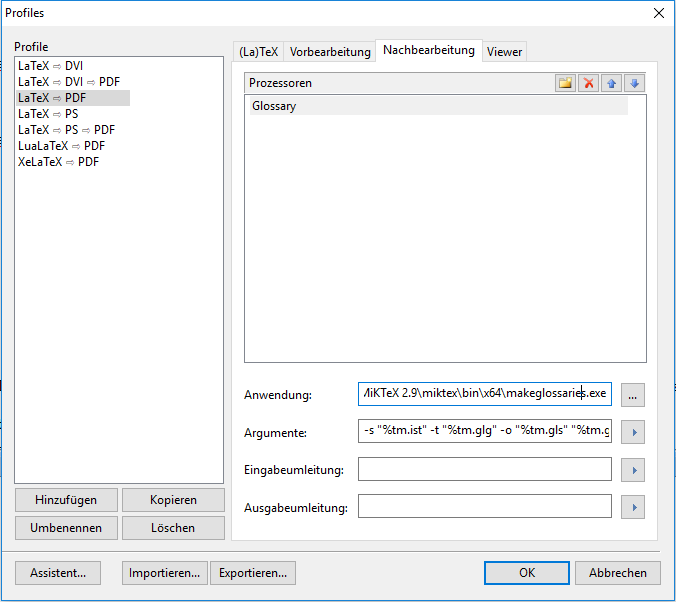
\includegraphics[width=\linewidth]{TeXnicCenterEinstellungenGlossar.PNG}
    \caption{Einstellungen für makeglossaries}
		\end{subfigure}
		\caption{Einstellungen für TeXnicCenter}
    \label{fig:Settings}
\end{figure}

\subsubsection{Mac~OS}

Unter Mac~OS wird die aktuelle Vorlage mangels verfügbarer Geräte nicht getestet. Der folgende Text bezieht sich auf die alte Vorlage und ist möglicherweise nicht mehr korrekt.

Bewährte und weit verbreitete Frontends für den Mac sind \emph{MacTeX}%
\footnote{\url{http://www.tug.org/mactex} -- enthält eine komplette und fertig
konfigurierte \latex\-Installation für Mac~OS\index[allgemein]{Mac~OS} (ca.\ 1.15 GB download).}
und \emph{TeXShop},%
\footnote{\url{http://www.uoregon.edu/~koch/texshop/}}
das üblicherweise zusammen mit der TeX-Distribution \emph{TeX Live} verwendet wird. 
Weit verbreitet ist auch der \emph{TeXworks} Editor, der ebenfalls im MacTeX Package enthalten ist und auch MiKTeX unter Windows beigefügt ist.

Weitere aktuelle Informationen zu der Arbeit mit \latex\ unter Mac~OS finden sich auf den Informationsseiten zu \latex\ der Technischen Universität Graz.\footnote{\url{http://latex.tugraz.at/programme/mac_os_x}}

\subsubsection{Linux}

Auch unter \gls{Linux}\index[allgemein]{Linux}  ist \emph{TeX Live} (\so) eine häufig verwendete TeX-Distri\-bution. 
Als Frontend sind beispielsweise
\emph{Texmaker}\footnote{\url{http://www.xm1math.net/texmaker}}(empfohlen) \emph{Lyx}\footnote{\url{http://www.lyx.org}},
\emph{Kile}\footnote{\url{http://kile.sourceforge.net}} und
verbreitet.
In manchen gängigen Linux-Versionen ist bereits eine komplette \latex-Distribution enthalten, sodass im besten Fall überhaupt keine zusätzliche Installation notwendig ist.  


Eine interessante Alternative ist die Verwendung von
\emph{Eclipse}\footnote{\url{http://www.eclipse.org}} als plattformunabhängiges Frontend 
(mit dem \emph{TeXlipse}\footnote{\url{http://texlipse.sourceforge.net}}
Plugin).


Zum Nachinstallieren zusätzlicher \latex-Pakete die nicht in der
Standardinstallation enthalten sind gibt es für Linux ebenfalls den MikTeX
Package Manager\footnote{\url{http://wiki.ubuntuusers.de/MiKTeX_Package_Manager}}. Allerdings empfiehlt es sich meist die notwendigen Pakete statt dessen über die Softwareverwaltung der Linux-Distribution zu installieren. So kann \zB\ in Ubuntu das Paket \emph{texlive-lang-german} installiert werden um die für diese Vorlage notwendige Unterstützung der deutschen Sprache nach zu installieren.


Wer es sich einfach machen will und kein Problem mit einem größeren Download bzw. größerem Speicherverbrauch auf der Festplatte hat, kann auch einfach \emph{TeX Live} mit dem Paket \emph{texlive-full} vollständig installieren.

\subsubsection{Automatische Generierung von \latex-Code}
Bei der Erstellung von komplizierterem \latex-Code kann man sich zum Glück
einiger Hilfsmittel bedienen.

\begin{itemize}
\item \emph{Online Latex Equation
Editor}\footnote{\url{http://www.codecogs.com/latex/eqneditor.php}} ist ein
einfach zu bedienender Online Editor für mathematische Formeln.
\item \emph{Online Latex Table Editor}\footnote{\url{http://www.tablesgenerator.com/latex_tables}}
\item \emph{Writer2\latex}\footnote{\url{http://www.ooowiki.de/Writer2LaTeX}}
ist ein Export-Filter für OpenOffice-Writer mit dem jede Form von Textdokumenten in
\latex-Code umgewandelt werden kann.
\item \emph{Calc2\latex}\footnote{\url{http://www.ooowiki.de/Calc2LaTeX}} ist
ein Export-Makro für OpenOffice-Calc mit dem Tabellen für das Einfügen in \latex
erzeugt werden können.
\item \emph{Dot2Tex}\footnote{\url{http://www.fauskes.net/code/dot2tex}} ist
eine Verbindung von Graphviz nach \latex. Graphen können in \latex eingebunden werden
und die Beschriftungen mit \latex geschrieben werden.
\item \emph{gnuplot}\footnote{\url{http://www.gnuplot.info}} ist ein Programm
zur Erstellen von Diagrammen. Über das \latex-Package gnuplottex kann es direkt in
den \latex-Code integriert werden.
\end{itemize}


\subsection{Literatur}
\label{sec:literatur}

Es ist müßig, ohne geeignete Literatur mit \latex zu beginnen, selbst
als fortgeschrittener Benutzer wird man immer wieder auf Hilfe angewiesen
sein. Erfreulicherweise ist sehr viel Nützliches auch online verfügbar.
Gute Startpunkte sind \zB
%
\begin{itemize}
\item \emph{\citetitle{Schmidt01}}\footcite{Schmidt01}
\item \emph{\citetitle{Oetiker01}}\footcite{Oetiker01}
\end{itemize}
%
\noindent
Als mittlerweile bereits klassisches Handbuch zu \latex ist
%
\begin{itemize}
  \item \emph{\citetitle{Kopka98}}\footcite{Kopka98}
\end{itemize}
%
zu empfehlen, zu dem es für Interessierte auch zwei vertiefende
Zusatzbände in Deutsch gibt. Zahlreiche weitere Dokumente zu
\latex und verwandten Themen finden sich \ua im Rahmen des {\em
Comprehensive TeX Archive Network} (CTAN) auf
\begin{quote}
	\url{http://www.ctan.org}%
	\footnote{\url{http://www.ctan.org/tex-archive/help/Catalogue/bytopic.html}}\newline
	\url{http://dante.ctan.org}%
	\footnote{\url{http://dante.ctan.org/tex-archive/help/Catalogue/bytopic.html}}\newline
	\url{http://www.tex.ac.uk}
\end{quote}
%
Besonders nützlich sind auch die
\emph{Comprehensive List of {\rm \latex} Symbols} \footcite{Pakin01}
und die Beschreibungen wichtiger \latex-Pakete, wie
%
\begin{quote}
	\texttt{babel} \footcite{Braams2008},\newline
  \texttt{grahics}, \texttt{graphicx} \footcite{Carlisle99},\newline
  \texttt{fancyhdr} \footcite{Oostrum97},\newline
  \texttt{caption} \footcite{Sommerfeldt07},\newline
  \texttt{subcaption} \footcite{Cochran95}.
\end{quote}


Und zu guter Letzt für die Freunde von Wikipedia gibt es noch ein \latex-Buch in der WikiBooks-Sammlung.\footnote{\url{https://en.wikibooks.org/wiki/LaTeX}}


\section{Schrift}

\subsection{Schriftarten}

\latex verwendet normalerweise die Schriften der \emph{Computer
Modern}
(CM) Serie, die so wie die \emph{TeX}-Software selbst von Donald Knuth%
\footnote{\url{http://www-cs-staff.stanford.edu/~knuth/}} entwickelt
wurden. Die drei Basis-Schrifttypen der CM-Serie in \latex sind
%
\begin{quote}
\begin{tabular}{lcl}
\textrm{Roman}      & & \verb!\textrm{Roman}!\\
\textsf{Sans Serif} & & \verb!\textsf{Sans Serif}!\\
\texttt{Typewriter} & & \verb!\texttt{Typewriter}!\\
\end{tabular}
\end{quote}
%
\noindent In den Augen vieler Benutzer ist allein die Qualität und
Zeitlosigkeit dieser Schriften ein Grund, \latex für seriöse
Zwecke zu verwenden. Ein weiterer Vorteil der \emph{TeX}-Schriften
ist, dass die unterschiedlichen Schriftfamilien und Schnitte
bezüglich der Größe sehr gut aufeinander abgestimmt sind, was %
beim Arbeiten mit verschiedenen \emph{TrueType}-Schriften (\zB\ in
\emph{Word}) durchaus zum Problem werden kann (\sa\ Kap.\
\ref{chap:Word}).

Darüber hinaus können aber in \latex auch beliebige 
\emph{PostScript}-Schrif\-ten (Type 1) verwendet werden, was allerdings in
der Praxis einiges an "`Tuning"'-Arbeit verlangt. Häufig verwendet
werden \zB\ \emph{Times} und \emph{Palatino}, derzeit ist aber ein Trend 
zurück zu den klassischen CM-Schriften zu beobachten.



\subsection{Texte hervorheben}

Texte können auf unterschiedliche Weise aus dem Fließtext hervorgehoben werden.
\begin{itemize}
%
\item Die Auszeichnung in \textit{Kursivschrift} oder "`italic"' (\verb!\textit{..}!) ist \va\ zum Hervorheben von
Betonungen und Zitaten geeignet, aber auch für
Produktbezeichnungen, Fremdwörter und Variablen im Text, \zB
%
\begin{quote}
\verb!\textit{Variable}! $\rightarrow$ \textit{Variable}
\end{quote}
%
\item {\sl Slanted} %
(\verb!\textsl{..}!) bedeutet eine geneigte Schrift und
unterscheidet sich damit deutlich von \textit{Italic}. Wird
beispielsweise verwendet für die laufenden Kopfzeilen,
Produktbezeichnungen und Markennamen -- zum Vergleich:
%
\begin{quote}
\verb!\textrm{Daimler-Chrysler}! $\rightarrow$ \textrm{Daimler-Chrysler} \newline%
\verb!\textsl{Daimler-Chrysler}! $\rightarrow$ \textsl{Daimler-Chrysler} \newline%
\verb!\textit{Daimler-Chrysler}! $\rightarrow$ \textit{Daimler-Chrysler}
\end{quote}
%
\item \textbf{Boldface} (\verb!\textbf{..}!) wird \ia\ verwendet für 
\textbf{Überschriften}, Bezeichnungen von \textbf{Abbildungen} und 
\textbf{Tabellen}, im Fließtext aber selten:
%
\begin{quote}
\verb!\textbf{Überschriften}! $\rightarrow$ \textbf{Überschriften}
\end{quote}
%
\item \emph{Emphasize} (\verb!\emph!) %
ist normalerweise gleichbedeutend mit \verb!\textit!, wobei
\verb!\emph{..}! allerdings auch bei geschachtelten
Hervorhebungen und im Bereich anderer Schriftschnitte das
"`Richtige"' tut: 
%
\begin{quote}
\setlength{\tabcolsep}{0pt}%
\begin{tabular}{lcl}
\verb!\textrm{Du \emph{auch} hier?}! & $\;\rightarrow\;$ &
    \textrm{Du \emph{auch} hier?}
\\
\verb!\textit{Du \emph{auch} hier?}! & $\;\rightarrow\;$ &
    \textit{Du \emph{auch} hier?} 
\\
\verb!\textsl{Du \emph{auch} hier?}! & $\;\rightarrow\;$ & 
    \textsl{Du \emph{auch} hier?}
\\
\verb!\textbf{Du \emph{auch} hier?}! & $\;\rightarrow\;$ & 
    \textbf{Du \emph{auch} hier?}
\\
\verb!\texttt{Du \emph{auch} hier?}! & $\;\rightarrow\;$ & 
    \texttt{Du \emph{auch} hier?}
\end{tabular}
\end{quote}
%
\item \underline{Unterstreichungen} sind ein Relikt aus der 
Schreibmaschinenära und im modernen Schriftsatz
eigentlich \underline{überflüssig}. Sie sollten daher nur in
Ausnahmefällen verwendet werden, \zB
%
\begin{quote}
\verb!\underline{überflüssig}!%
\footnote{Unterstrichene Texte werden zudem nicht automatisch abgeteilt.}
\end{quote}
%
\end{itemize}



\section{Textstruktur}

\subsection{Absatztrennung}

Absätze werden in {\latex}-Quelltext ausschließlich durch das
Einfügen einer oder mehrerer \textbf{Leerzeilen} voneinander
getrennt, es sind also \emph{keinerlei sonstige Steueranweisungen}
notwendig!
%
\begin{center}
\setlength{\fboxrule}{0.2mm}
\setlength{\fboxsep}{2mm}
\fbox{%
\begin{minipage}{0.9\textwidth}
Besonders die Verwendung von \texttt{\textbackslash\textbackslash} und 
 \texttt{\textbackslash{newline}}
Anweisungen zur Absatztrennung ist ein häufig zu beobachtender \textbf{Fehler}. 
Vor normalen Absätzen auch \emph{nichts} verloren hat die
Anweisung \texttt{\textbackslash{paragraph}\{\}}
-- sie ist in \latex\ (im Unterschied zu HTML)
eine Markierung für Überschriften mit Titel (\su)!
\end{minipage}}
\end{center}

Üblicherweise wird durch {\latex} zwischen aufeinander folgenden Ab\-sätzen
\emph{kein} zusätzlicher vertikaler Abstand eingefügt. \footnote{Das ist die
Standardeinstellung in {\latex} und natürlich abhängig von der verwendeten Dokumentenklasse, Style
etc.} 
Allerdings wird die
\emph{erste} Zeile jedes Absatzes (mit Ausnahme des ersten Absatzes
eines Abschnitts) eingerückt, um so die Absatzgrenzen deutlich zu
machen. Dieses Schema hat sich nicht nur im traditionellen
Buchsatz bewährt%
\footnote{Wer es nicht glaubt, sollte sein Bücherregal (oder notfalls das seiner Eltern) nach Gegenbeispielen durchsuchen.}
und sollte auch beibehalten werden, es sei denn
man hat wirklich \emph{sehr} gute Gründe dagegen.
Für alle übrigen Gliederungen im vertikalen Textfluss sind Überschriften (s.\ unten) vorgesehen.

\SuperPar 
Manchmal besteht allerdings der Wunsch, etwa zur Verdeutlichung eines inhaltlichen Sprungs \emph{zwischen} zwei Absätzen einen zusätzlichen Abstand einzufügen, ohne dabei eine neue Überschrift zu setzen. Das kann man gegebenenfalls (wie vor dem aktuellen Absatz passiert) durch 
%
\begin{quote}
\texttt{{\bs}SuperPar} \emph{Manchmal besteht allerdings der Wunsch, \ldots}
\end{quote}
%
erreichen, sollte jedoch sehr sparsam und wirklich \textbf{nur in begründbaren Einzelfällen} verwendet werden.%
\footnote{Das Makro \texttt{{\bs}SuperPar} ist in \texttt{htl.sty} definiert.}




\subsection{Überschriften}
\label{sec:ueberschriften}

\latex\ bietet -- abhängig von der verwendeten Dokumentenklasse --
einen Satz vordefinierter Überschriftformate in folgender Ordnung:
%
\begin{quote}
\verb!\part{!\texttt{\em Titel}\verb!}!%
\footnote{\texttt{part} ist für die Gliederung eines
größeren Werks in mehrere Teile vorgesehen und wird üblicherweise
bei einer Diplomarbeit (und auch in diesem Dokument) nicht
verwendet.}
\newline%
\verb!\chapter{!\texttt{\em Titel}\verb!}! \newline%
\verb!\section{!\texttt{\em Titel}\verb!}! \newline%
\verb!\subsection{!\texttt{\em Titel}\verb!}! \newline%
\verb!\subsubsection{!\texttt{\em Titel}\verb!}! \newline%
\verb!\paragraph{!\texttt{\em Titel}\verb!}! \newline%
\verb!\subparagraph{!\texttt{\em Titel}\verb!}!
\end{quote}
%

\paragraph{Häufiger Fehler:} Bei \verb!\paragraph{}! und
\verb!\subparagraph{}! läuft -- wie in diesem Absatz zu sehen --
der dem Titel folgende Text ohne Umbruch in der selben Zeile
weiter, weshalb man im Titel auf eine passende Punktuation (hier
\zB\ \underline{\texttt{:}}) achten sollte. Der horizontale Abstand
nach dem Titel allein würde diesen als Überschrift nicht erkennbar
machen.


\subsection{Listen}

Listen sind ein beliebtes Mittel zur Textstrukturierung. In
\latex\ sind -- ähnlich wie in HTML -- drei Arten von formatierten
Listen verfügbar: ungeordnete Auflistung ("`Knödelliste"'),
geordnete Auflistung (Aufzählung) und Beschreibungsliste
(Description):
%
\begin{verbatim}
    \begin{itemize}     ... \end{itemize}
    \begin{enumerate}   ... \end{enumerate}
    \begin{description} ... \end{description}
\end{verbatim}
%
Listeneinträge werden jeweils mit \verb!\item! markiert, bei {\tt
description}-Listen mit \verb!\item[!\texttt{\em titel}\verb!]!. Listen
können ineinander verschachtelt werden, wobei sich bei {\tt
itemize}- und \texttt{enumerate}-Listen die Aufzählungszeichen mit
der Schachtelungstiefe ändern (Details dazu in der
\latex-Dokumentation).


\subsection{Absatzformatierung und Zeilenabstand}

Diplomarbeiten werden -- wie Bücher -- in der Regel einspaltig und
im Blocksatz formatiert, was für den Fließtext wegen der großen
Zeilenlänge vorteilhaft ist. Innerhalb von Tabellen kommt es
wegen der geringen Spaltenbreite jedoch häufig zu Problemen mit
Abteilungen und Blocksatz, weshalb man dort ohne schlechtes
Gewissen zum Flattersatz ("`ragged right"') greifen sollte (wie
\zB\ in Tab.~\ref{tab:synthesis-techniques} auf Seite
\pageref{tab:synthesis-techniques}).

\subsection{Fußnoten}
Fußnoten können in \latex\ an beinahe jeder beliebigen Stelle,
jedenfalls aber in normalen Absätzen, durch die Anweisung
%
\begin{quote}
\verb!\footnote{!\texttt{\em Fußnotentext}\verb!}!
\end{quote}
%
gesetzt werden. Zwischen der \verb!\footnote!-Marke und dem davor
liegenden Text sollte grundsätzlich \emph{kein Leerzeichen} entstehen (eventuelle
Zeilen\-um\-brüche mit \verb!%! auskommentieren).
Die Nummerierung und Platzierung der Fußnoten
erfolgt automatisch, sehr große Fußnoten werden notfalls sogar auf
zwei aufeinander folgende Seiten umgebrochen.


\subsubsection{Fußnoten in Überschriften}

Auch das braucht man ab und zu, ist aber \va\ deshalb kein so
einfacher Fall, weil die Fußnote in einer Überschrift nur an Ort
und Stelle auf scheinen darf, nicht aber im \emph{Inhaltsverzeichnis}! Ein
konkretes Beispiel dafür ist die Überschrift zu
Kapitel~\ref{chap:Word}, die etwa folgendermaßen definiert ist:
%
\begin{quote}
\begin{verbatim}
\chapter[Hinweise für Word-Benutzer]%
        {Hinweise für Word-Benutzer%
        \protect\footnote{Dieser Abschnitt ....}}%
\end{verbatim}
\end{quote}
%
Dabei ist der erste (optionale) Titel \verb![Hinweise für ...]!
der Eintrag im Inhaltsverzeichnis und im Seitenkopf. 
Der zweite (identische) Titel
\texttt{\{Hinweise für ...\}} erscheint auf der aktuellen Seite und
enthält auch den \verb!\footnote{}! Eintrag, der allerdings an
dieser Stelle durch die Direktive \verb!\protect! "`geschützt"'
werden muss. Die \verb!%!-Zeichen sind übrigens notwendig,
um eventuelle Leerzeichen, die durch Zeilenumbrüche im Quelltext
entstehen, zu eliminieren (diesen Trick braucht man %
in \latex\ häufig, s.\ Abschn.~\ref{sec:kommentare}). 
Ziemlich kompliziert also, und damit 
ein weiterer Grund, Fußnoten an solchen Stellen überhaupt zu vermeiden.

Generell sollte man mit Fußnoten sparsam umgehen, da sie den
Textfluss unterbrechen und den Leser ablenken. Insbesondere
sollten Fußnoten nicht (wie \va\ in manchen
sozialwissenschaftlichen Werken gepflegt) derart lang werden, dass
sie einen Großteil der Seite einnehmen und damit praktisch ein
zweites Dokument bilden.%
\footnote{Das führt bei Dokumenten mit vielen Fußnoten bei manchen Lesern angeblich so weit, dass sie aus Neugier (oder Versehen) regelmäßig bei den Fußnoten zu lesen beginnen und dann mühevoll die zugehörigen, kleingedruckten Verweise im Fließtext suchen.}


\subsection{Querverweise}
\label{sec:querverweise}

Zur Verwaltung von Querverweisen innerhalb eines Dokuments stellt
\latex\ einen sehr einfachen Mechanismus zur Verfügung. Zunächst
muss jede Stelle (Kapitel, Abschnitt, Abbildung, Tabelle etc.)
durch
%
\begin{quote}
\verb!\label{!\texttt{\em key}\verb!}!
\end{quote}
%
markiert werden, wobei \texttt{\em key} ein gültiges \latex-Symbol sein
muss. Damit Labels (die nur Zahlen sind) nicht verwechselt werden,
ist es üblich, sie je nach Bedeutung mit einer unterschiedlichen
Prefix zu versehen, \zB\
%
\begin{quote}
\tabcolsep0pt
\begin{tabular}{ll}
\verb!cha:!\texttt{\em kapitel}   & \ \ldots\ für Kapitel  \\
\verb!sec:!\texttt{\em abschnitt} & \ \ldots\ für Abschnitte (Sections) und Unterabschnitte \\
\verb!fig:!\texttt{\em abbildung} & \ \ldots\ für Abbildungen \\
\verb!tab:!\texttt{\em tabelle}   & \ \ldots\ für Tabellen \\
\verb!equ:!\texttt{\em gleichung} & \ \ldots\ für Formeln und Gleichungen\\
\end{tabular}
\end{quote}
%
\noindent Beispiele:\ \verb!\label{cha:Einleitung}! oder
\verb!\label{fig:Screen-1}!. Mit den Anweisungen
%
\begin{quote}
\verb!\ref{!\texttt{\em key}\verb!}! 
\hspace{1em} oder \hspace{1em} 
\verb!\pageref{!\texttt{\em key}\verb!}!
\end{quote}
%
kann an beliebiger Stelle im Dokument die zu \texttt{\em key} gehörige
Nummer bzw.\ Seitennummer eingesetzt werden, \zB\
%
\begin{quote}
\verb!.. wie in Kap.~\ref{cha:Einleitung} erwähnt ..!\\
\verb!.. der Screenshot auf Seite \pageref{fig:Screen-1} ..!
\end{quote}
%
Übrigens werden die Bezeichnungen \emph{Kapitel} und {\em
Abschnitt} auffallend oft falsch verwendet -- Kapitel haben
ausschließlich "`ungebrochene"' Nummern:
%
\begin{quote}
\begin{tabular}{ll}
   \textrm{Richtig:\ } & Kapitel 7 oder Abschnitt 2.3.4\\
   \textbf{Falsch:\ }  & Kapitel 7.2 oder Abschnitt 5
\end{tabular}
\end{quote}


\section{Wortabstand und Punktuation}

\subsection{\emph{French Spacing}}
Im englischsprachigen Schriftsatz ist es üblich, nach jedem
Satzende einen gegenüber dem normalen Wortzwischenraum
vergrößerten Abstand einzusetzen. Obwohl dies im Deutschen und
Französischen traditionell nicht so ist, wird es wegen der
verbesserten Lesbarkeit auch hier manchmal verwendet (nicht in diesem
Dokument). Falls man die englische ("`nicht-französische"') Satztrennung mit
zusätzlichem Abstand bevorzugt, ist lediglich die Zeile
%
\begin{quote}
\verb!\nonfrenchspacing!
\end{quote}
%
am Beginn des Dokuments einzusetzen. 
In diesem Fall sollte man 
aber die Interpunktion innerhalb von
Sätzen (nach .\ und :) sorgfältig beachten. Beispielsweise
schreibt man "`Dr.\ Mabuse"' in der Form
%
\begin{quote}
\verb!Dr.\ Mabuse! oder \verb!Dr.~Mabuse!
\end{quote}
%
Im zweiten Beispiel wird mit \verb!~! zudem ein Zeilenumbruch am Leerzeichen verhindert.


\subsection{Gedanken- und Bindestriche}
\label{sec:gedankenstrich}

Die Verwendung der falschen Strichlängen (mit und ohne
Zwischenraum) ist ganz allgemein eine häufige Fehlerquelle.
Bewusst unterscheiden sollte man zwischen
%
\begin{itemize}
\item kurzen Bindestrichen (wie in "`Wagner-Jauregg"'), %
\item Minus-Zeichen, \zB\ $-7$ (erzeugt mit \verb!$-7$!), und %
\item echten Gedankenstrichen -- wie hier (erzeugt mit \verb!--!).
\end{itemize}
%
\noindent Für das Setzen von Gedankenstrichen\footnote{Für alle
drei gibt es übrigens auch in \emph{Word} entsprechende
Sonderzeichen.} gibt es eindeutige Konventionen:
%
\begin{enumerate}
\item Im \emph{Deutschen} setzt man üblicherweise einen von zwei
Leerzeichen umgebenen Gedankenstrich%
\footnote{Halbgeviertstrich (\emph{En Dash}).} -- wie hier (in
\latex\ mit {\verb*! -- !}). Dieser wird auch für die Angabe von
Zahlenintervallen (Seiten 12--19) benutzt. 
%
\item In \emph{englischen} Texten verwendet man einen noch längeren
Gedankenstrich\footnote{Geviertstrich (\emph{Em Dash}).} \emph{ohne}
zusätzliche Leerzeichen---\emph{as we should be knowing by now}
(in \latex\ mit {\verb*!---!}).
%
\end{enumerate}




\subsection{Kommentare}
\label{sec:kommentare}


Textteile können in \latex\ zeilenweise mit \verb!%! auskommentiert werden. Der einem 
\verb!%!-Zeichen nachfolgenden Text wird bis zum nächsten Zeilenende überlesen:
%
\begin{quote}
\verb!Das wird gedruckt. %Dieser Text wird ignoriert.!
\end{quote}
%
Häufig verwendet werden Kommentarzeichen aber auch zum Ausblenden von 
\emph{white space}, also Leerzeichen und Zeilenumbrüchen.
Folgendes Beispiel zeigt etwa, wie man mit \verb!%! am Zeilendende das Entstehen
eines Leerzeichens vor einer nachfolgenden Fußnotenmarke vermeiden kann:
%
\begin{quote}
\begin{verbatim}
In Österreich isst man sonntags Schnitzel.%
\footnote{Was die allgemein gute Kondition erklärt.}
\end{verbatim}
\end{quote}
%

\begin{sloppypar}
\noindent
Auf ähnliche Weise kann man das Entstehen von ungewolltem Absatz\-zwischenraum durch 
gezielten Einsatz von Kommentarzeilen vermeiden, \zB\ vor und nach einem zentrierten
Textabschnitt:
\end{sloppypar}
%
\begin{quote}
\begin{verbatim}
... normaler Text.
%
\begin{center}
   Dieser Test ist zentriert.
\end{center}
%
Und jetzt geht es normal weiter ...
\end{verbatim}
\end{quote}
%
Darüber hinaus bietet die \verb!comment!-Umgebung die Möglichkeit, größere Text\-blöcke
in einem Stück auszublenden:
%
\begin{quote}
\begin{verbatim}
\begin{comment}
Dieser Text ...
   ... wird ignoriert.
\end{comment}
\end{verbatim}
\end{quote}




\subsection{Anführungszeichen}
\label{sec:anfuehrungszeichen}

Mit Anführungszeichen geht man aus Gewohnheit meist etwas
nachlässig um; auch dabei sind aber die Unterschiede zwischen Deutsch
und Englisch zu beachten. Hier die richtige \latex-Notation für
beide Sprachen:
%
\begin{quote}
\verb!``English''! $\rightarrow$ ``English'' \\
\verb!"`Deutsch"'! $\rightarrow$ "`Deutsch"' 
\end{quote}
%
Bei richtiger Einstellung werden beispielsweise im TeXnicCenter-Editor und im
Eclipse-Plugin Texlipse die entsprechenden Zeichenfolgen automatisch
eingesetzt. \emph{Einfache} Anführungszeichen erzeugt man im Englischen analog, im Deutschen benötigt man dafür die Makros \verb!\glq! \bzw\ \verb!\grq! (German left/right quote):
\begin{quote}
\verb!`English'! $\rightarrow$ `English' \\
\verb!{\glq}Deutsch{\grq}! $\rightarrow$ {\glq}Deutsch{\grq} 
\end{quote}





\section{Abteilen}
\label{subsec:layout-abteilen}

Um ein sauberes Schriftbild zu erreichen sind -- speziell im
Deutschen wegen der großen Wortlängen -- Abteilungen
(Silbentrennung, Hyphenation) unerlässlich, entweder manuell durch
Einfügen von optionalen Trennzeichen oder automatisch. In \latex
wird grundsätzlich automatisch abgeteilt, wobei die Sprache am
Beginn des Dokuments festgelegt und entsprechende Abteilungsregeln
für den gesamten Text verwendet werden.

Besonders bei schmalen Textspalten kann es vorkommen, dass \latex
keine geeignete Stelle für den Zeilenumbruch findet und den Text
über den rechten Rand hinaus laufen lässt. Das ist durchaus
beabsichtigt und soll anzeigen, dass an dieser Stelle ein Problem
besteht, das man durch manuelles Eingreifen reparieren muss.

Generell sollte man gegenüber der automatischen Abteilung
misstrauisch sein und das Endergebnis stets sorgfältig überprüfen.
Vor allem Wörter mit Umlauten oder Bindestrichen werden in \latex\ 
oft unrichtig abgeteilt.
Bei Bedarf kann man mit \verb!\-! gezielt zulässige Abteilungspunkte 
definieren, wie \zB\ in
%
\begin{quote}
\verb!Fach\-hoch\-schul\-kon\-fe\-renz!.
\end{quote}
%
In echten Problemfällen -- etwa bei Schwierigkeiten mit Textelementen, die nicht umgebrochen 
werden dürfen oder können -- kann man \latex\ dazu veranlassen, in einzelnen Absätzen
etwas weniger pingelig zu formatieren. Das erreicht man durch
%
\begin{quote}
\begin{verbatim}
\begin{sloppypar}
    Dieser Absatz wird ``schlampig'' (sloppy) gesetzt ...
\end{sloppypar}
\end{verbatim}
\end{quote}
%
Der letzte Rettungsanker ist, den betreffenden Absatz so umzuschreiben, dass sich ein passabler Zeilenumbruch ergibt (schließlich ist man ja selbst der Autor und niemandem eine
Rechtfertigung schuldig).%
\footnote{Angeblich waren eigenständige Textänderungen in solchen Fällen auch beim früheren Bleisatz durchaus üblich.}



\section{Das {\tt htl}-Paket}

Diesem Dokument angeschlossen sind zwei Dateien, die beide zum Erstellen dieses Dokuments erforderlich sind:
%
\begin{description}
\item[\url{htldipl.cls} (class file):] definiert die 
		Dokumentenstruktur, Layout und den gesamten Vorspann des Dokuments (Titelseite etc.).
\item[\url{htl.sty} (style file):] enthält nützliche 
		Definitionen. Diese Datei wird von \url{htldipl.cls} automatisch geladen, kann 
		aber grundsätzlich auch für andere Dokumente verwendet werden.
\end{description}


\subsection{Einstellungen}


Alle (\verb!.tex!) Dokumente dieser Klasse beginnen mit der Anweisung
%
\begin{itemize}
\item[] \verb!\documentclass[!\texttt{\emph{language,printsetting,colormode}}\verb!]{htldipl}! 
\end{itemize}
%
Mit der Option \texttt{\emph{language}} kann die Hauptsprache des Dokuments spezifiziert werden, 
die möglichen Werte dafür sind
%
\begin{itemize}
\item[] \verb!german! (\emph{default})
\item[] \verb!english!
\end{itemize}

Mit der Option \texttt{\emph{printsetting}} kann spezifiziert werden, ob das Dokument im Druck einseitig oder beidseitig gedruckt werden soll. Diese Option steuert natürlich nicht direkt den Drucker, sondern passt die Formatierung des Dokuments für den späteren Druck an. \ZB\ werden bei bedarf Leerseiten hinzugefügt, damit bei beidseitigem Druck die Kapitel immer auf der Vorderseite beginnen.
Die möglichen Werte dafür sind
%
\begin{itemize}
\item[] \verb!oneside! (\emph{default})
\item[] \verb!twoside!
\end{itemize}
%
Mit der Option \texttt{\emph{colormode}} kann spezifiziert werden, ob der im Dokument enthaltene Source-Code mit farblichem Syntax-Highlighting dargestellt werden soll oder in Grau/Schwarz. Wird das ganze Dokument auf einem Farbdrucker gedruckt empfiehlt sich die farbliche Darstellung. Werden nur die Seiten mit Farbbildern auf einem Farbdrucker gedruckt sollte für die bessere Lesbarkeit des Codes die andere Darstellung gewählt werden.
Die möglichen Werte dafür sind
%
\begin{itemize}
\item[] \verb!color! (\emph{default})
\item[] \verb!black!
\end{itemize}
%
Der vollständige Quelltext für eine entsprechende \verb!.tex! Hauptdatei ist in Anhang \ref{app:latex} 
gelistet.


\subsubsection{Angaben zur Arbeit}

Zum erstellen der Titelseite sind einige Angaben notwendig \zB\:
%
\begin{itemize}
\item[] %
\verb!\title{!\texttt{\em Titel der Arbeit}\verb!}! \newline%
\verb!\abteilung{!\texttt{\em Abteilung}\verb!}! \newline%
\verb!\studienort{!\texttt{\em Studienort}\verb!}! \newline%
\verb!\abgabejahr{!\texttt{\em Jahr der Abgabe}\verb!}!
\end{itemize}
%

Da die Diplomarbeit von einer unterschiedliche Anzahl von Autoren geschrieben werden kann, können bei den Angaben zu den Autoren die nicht benötigten Einträge einfach frei gelassen werden.


\subsubsection{Titelseiten}

Die ersten Seiten der Arbeit, einschließlich der Titelseite,
werden durch die Anweisung
\begin{itemize}
\item[] %
\verb!\maketitle!  
\end{itemize}
automatisch generiert, abhängig von den obigen
Einstellungen:
%
\begin{center}
\begin{tabular}{cll}
\emph{Seite} & \emph{Diplomarbeit} \\
  \hline
  {\rm i} & Titelseite \\
  {\rm ii} & Eidesstattliche Erklärung \\
  \hline
\end{tabular}
\end{center}






\subsection{Definierte Abkürzungen}

Es wird im \texttt{htl}-Paket weiters eine Reihe von Abkürzungsmakros%
\footnote{In Anlehnung an den \texttt{jkthesis}-Style von Jochen
Küpper (\url{http://www.jochen-kuepper.de}).} definiert, die das
Schreiben vereinfachen und für konsistente
Zwisch\-en\-ab\-stän\-de sorgen (Tab.~\ref{tab:abkuerzungen}).
Bei der Verwendung von Makros ist allgemein zu beachten, dass sie nachfolgende Leerzeichen bisweilen "`auffressen"', sodass vor dem nachfolgenden Text kein Abstand erzeugt wird.%
\footnote{Bei den meisten der in \texttt{htl.sty} definierten Makros wird dies
allerdings durch den Einsatz von \texttt{\textbackslash xspace} verhindert.} Dagegen kann man sich mit \verb!\!-Zeichen oder \verb!{}! behelfen, wie in folgendem 
(nicht sehr schönen) Beispiel:
%
\begin{itemize}
\item[] \verb!Mopeds und Autos haben \ia\ zwei {\bzw} vier Räder.!\\
      Mopeds und Autos haben \ia\ zwei {\bzw} vier Räder.
\end{itemize}


\begin{table}
\caption{In \texttt{htl.sty} definierte Abkürzungsmakros.}
\label{tab:abkuerzungen}
\centering
\begin{tabular}{llp{2cm}ll}
\hline
    \verb+\bzw+        & \bzw   & &  \verb+\ua+         & \ua \\
    \verb+\bzgl+       & \bzgl  & &  \verb+\Ua+         & \Ua \\
    \verb+\ca+         & \ca    & &  \verb+\uae+        & \uae \\
    \verb+\dah+        & \dah   & &  \verb+\usw+        & \usw \\
    \verb+\Dah+        & \Dah   & &  \verb+\uva+        & \uva \\
    \verb+\ds+         & \ds    & &  \verb+\uvm+        & \uvm \\
    \verb+\evtl+       & \evtl  & &  \verb+\va+         & \va \\
    \verb+\ia+         & \ia    & &  \verb+\vgl+        & \vgl \\
    \verb+\sa+         & \sa    & &  \verb+\zB+         & \zB \\
    \verb+\so+         & \so    & &  \verb+\ZB+         & \ZB \\
    \verb+\su+         & \su    & &                     &     \\
\hline
\end{tabular}
\end{table}




\subsection{Sprachumschaltung}
\label{sec:sprachumschaltung}

Für englischsprachige Abschnitte (\zB\ das Abstract oder englische
Zitate) sollte die \emph{Sprache} von Deutsch auf Englisch
umgeschaltet werden, um die richtige Form der Silbentrennung zu
erhalten. Damit man nicht versehentlich auf das Rückstellen der
Sprache vergisst, sind dafür im \texttt{htl}-Paket zwei
spezielle \emph{Environments} vorgesehen:
%
\begin{itemize}
\item[] 
\verb!\begin{english}!\\
\verb!    This is a 1-page (maximum) summary!\\
\verb!    of your work in English.!\\
\verb!\end{english}!
\end{itemize}

\begin{itemize}
\item[] 
\verb!\begin{german}!\\
\verb!    Text in Deutsch (wenn die Hauptsprache!\\
\verb!    auf Englisch gesetzt ist).!\\
\verb!\end{german}!
\end{itemize}
%
Zur Kontrolle lässt sich aktuelle Spracheinstellung übrigens mit dem Makro \verb!\languagename!
anzeigen. An dieser Stelle ergibt das beispielsweise "`\texttt{\languagename}"' (\emph{new german}, \dah\ neue deutsche Rechtschreibung).


\subsection{Zusätzliche {\latex}-Pakete}

Für die Verwendung dieses Dokuments ist eine Reihe von
zusätzlichen \latex-Paketen erforderlich
(Tab.~\ref{tab:packages}). Diese Pakete werden am Anfang
durch das \texttt{htl}-Paket automatisch geladen. 
Alle verwendeten Pakete sind
Teil der \latex\ Standard-Installation, wie \zB in MikTeX, wo
man auch entsprechende Dokumentation findet (meist als DVI-Dateien).
Die aktuellen Versionen der Pakete sind online verfügbar, \ua\ auf den
in Abschn.~\ref{sec:literatur} angegebenen CTAN-Sites.

\begin{table}
\caption{Im \texttt{htl}-Paket verwendeten \latex-Ergänzungen. Alle sind in
gängigen \latex\ Standardinstallationen (\zB MikTeX) bereits enthalten.}
\label{tab:packages}
\centering\small
\tabcolsep2pt
\begin{tabular}{ll}
%\hline
\emph{Paket} &  \emph{Funktion} \\
\hline
\texttt{algorithmicx} & Beschreibung von Algorithmen \\ 
\texttt{amsfonts}, \texttt{amsbsy}   &  Mathematische Symbole \\ 
\texttt{amsmath}  &  Mathematischer Schriftsatz \\ 
\texttt{babel}  	&  Sprachumschaltung \\ 
\texttt{babelbib} &  Mehrsprachige Literaturverwaltung \\ 
\texttt{caption}  &  Flexiblere Captions \\ 
\texttt{cite}     &  Sortierte Literaturverweise \\ 
\texttt{color}    &  Farbige Textelemente und Hintergrundfarben \\ 
%\texttt{eurosym}  &  {\euro}-Symbol (\verb!\euro!)\\ 
\texttt{marvosym}  &  {\euro}-Symbol (\verb!\euro!)\\ 
\texttt{exscale}  &  Korrekte Schriftgrößen im Math-Modus \\ 
\texttt{fancyhdr} &  zur Gestaltung Kopfzeilen (header) \\ 
\texttt{float}    &  Verbessertes Float-Handling \\ 
\texttt{fontenc}  &  zur Verwendung der cm-super Type1 Postscript Schriften \\ 
\texttt{graphicx} &  Einbindung von EPS-Grafiken \\ 
\texttt{hyperref} &  erzeugt aktive Querverweise im PDF-Dokument \\ 
\texttt{ifthen}   &  für logische Entscheidungen in \latex\\
\texttt{inputenc} &  Erweiterter Eingabezeichensatz \\ 
%\texttt{latin1}   &  T1-Schriften, \ua zur besseren Silbentrennung \\ 
\texttt{listings-utf8} &  Auflistung von Programmcode \\ 
\texttt{pdfpages}  &  PDF-Seiten in das Dokument einbinden \\ 
\texttt{upquote}  &  Gerade Hochkommas in \texttt{verbatim}-Texten \\ 
\texttt{url}      &  Behandlung von URLs im Text \\ 
\texttt{verbatim} &  Verbesserte \texttt{verbatim}-Umgebung \\
\hline
\end{tabular}
\end{table}





\section{\latex-Fehlermeldungen und Warnungen}

Während des Durchlaufs gibt \latex\ Unmengen von
Meldungen aus, die einen in ihrer Fülle zunächst nicht verwirren
sollten, \zB:

\begin{scriptsize}
\begin{verbatim}
...
Overfull \hbox (14.43593pt too wide) in paragraph at lines 105--109
\OT1/cmr/m/n/10.95 F[]ur die Ein-bin-dung von Gra-phi-ken in L[]T[]X wird die V
er-wen-dung des Standard-
[10] [11]
Overfull \hbox (5.01222pt too wide) in paragraph at lines 148--154
\OT1/cmr/m/n/10.95 wen-di-gen Ras-te-rung kei-nen Sinn, auch bei 1200 dpi-Druck
ern. Spe-zi-ell \OT1/cmr/m/it/10.95 Screen-
...
\end{verbatim}
\end{scriptsize}
%
\emph{Errors} (Fehler) müssen korrigiert werden, wobei einem \latex\ diese Arbeit 
nicht leicht macht, da manchmal (\zB\ wenn eine schließende Klammer \verb!}! 
vergessen wurde) das Problem erst viel später im Text lokalisiert wird.
In solchen Fällen kann es nützlich sein, das erzeugte Ausgabedokument
zu inspizieren um festzustellen, ab welcher Stelle die Ergebnisse
aus dem Ruder laufen.  
Bei kapitalen Fehlern bleibt der \latex-Prozessor überhaupt stehen und 
erzeugt keine Ausgabe (in Verbindung mit einer meist kryptischen
Fehlermeldung) -- hier hilft meist nur eine genaue
Analyse des Quelltexts oder der gerade zuvor durchgeführten Schritte.
Ein ausführliches Fehlerprotokoll findet man jeweils in der \verb!.log!-Datei 
des Hauptdokuments.

Falls keine Fehler mehr angezeigt werden, ist zumindest die syntaktische Struktur
des Dokuments in Ordnung.
Genauer ansehen sollte man sich die Liste von Meldungen jedoch
spätestens beim Abschluss der Arbeit, um übrig gebliebene Probleme, wie
überlange Textzeilen, unaufgelöste Verweise und ähnliche zu
beseitigen.
Am Ende sollte das Ergebnis jedenfalls so ausehen:
%
\begin{quote}
\verb!LaTeX-Result: 0 Error(s), 0 Warning(s), ...!
\end{quote}
\chapter{Abbildungen, Tabellen, Quellkode}
\label{chap:Abbildungen}

\section{Allgemeines}

Abbildungen (\emph{figures}) und Tabellen (\emph{tables}) werden üblicherweise
zusammen mit einem nummerierten Titel (\emph{caption}) zentriert
angeordnet (siehe Abb.~\ref{fig:urlaub}).
Im Text \emph{muss} es zu jeder Abbildung einen Verweis geben und die eigentliche Abbildung
sollte erst \emph{nach} dem ersten Verweis platziert werden.

\begin{figure}
\centering
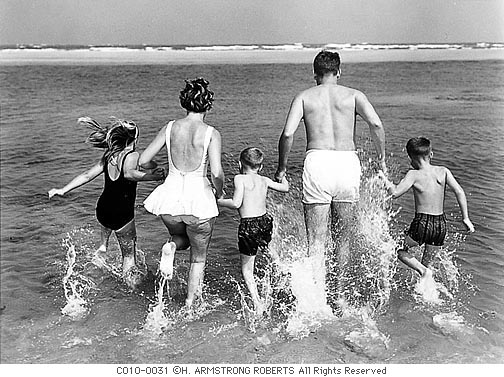
\includegraphics[width=.85\textwidth]{CS0031}
\caption{Newport Beach 1957.}
\label{fig:urlaub}
\end{figure}



\section{\emph{Let Them Float!}}

Das Platzieren von Abbildungen und Tabellen gehört zu den
schwierigsten Aufgaben im Schriftsatz, weil diese meist viel Platz
benötigen und häufig nicht auf der aktuellen Seite im laufenden
Text untergebracht werden können. Diese Elemente müssen daher an
eine geeignete Stelle auf nachfolgenden Seiten verschoben werden,
was manuell sehr mühsam (jedoch in \emph{Word} beispielsweise unerlässlich) ist.

In \latex funktioniert das weitgehend automatisch, indem
Abbildungen, Tabellen und ähnliche als "`Floating Bodies"'
behandelt werden. Bei der Positionierung dieser Elemente wird
versucht, einerseits im Textfluss möglichst wenig Leer\-raum
entstehen zu lassen und andererseits die Abbildungen und Tabellen
nicht zu weit von der ursprünglichen Textstelle zu entfernen.

Der Gedanke, dass etwa Abbildungen kaum jemals genau an der
ge\-wünsch\-ten Stelle und möglicherweise nicht einmal auf
derselben Seite Platz finden, ist für viele Anfänger aber offenbar sehr
ungewohnt oder sogar beängstigend. Dennoch sollte man zunächst einmal
getrost \latex\ diese Arbeit überlassen und \emph{nicht} manuell
eingreifen. Erst am Ende, wenn das gesamte Dokument "`steht"' und
man mit der automatischen Platzierung wirklich nicht zurande
kommt, sollte man (durch gezielte Platzierungsanweisungen
\cite[S.~33]{Oetiker01}) \textbf{in Einzelfällen} eingreifen.



\section{Captions}

Bei Abbildungen steht der Titel üblicherweise \emph{unten}, bei
Tabellen hingegen -- je nach Konvention -- \emph{oben} (wie in diesem Dokument) 
oder ebenfalls \emph{unten}. In \latex\ erfolgt
auch die Nummerierung der Abbildungen automatisch, ebenso der
Eintrag in das (optionale)
Abbildungsverzeichnis%
\footnote{Ein eigenes Verzeichnis der Abbildungen am Anfang des Dokuments
ist zwar leicht erstellt, in einer Diplomarbeit aber (und eigentlich
überall sonst auch) überflüssig. Man sollte es daher weglassen.}
am Beginn des Dokuments.

Die Markierung der Captions%
\footnote{Ausnahmsweise wird das Wort "`Caption"' im Folgenden
ohne deutsche Übersetzung verwendet.} erfolgt in \latex mithilfe
der \verb!\label{}! Anweisung, die unmittelbar auf die
\verb!\caption{}! Anweisung folgen muss:
%
\begin{LaTeXCode}
\begin{figure}
\centering
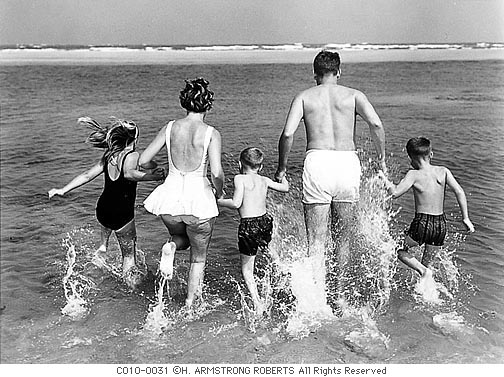
\includegraphics[width=.85\textwidth]{CS0031}
\caption{Newport Beach 1957.}
\label{fig:urlaub}
\end{figure}
\end{LaTeXCode}
%
Der Name des Labels (\texttt{fig:urlaub}) kann beliebig gewählt werden. 
Die Kennzeichnung \texttt{fig:} ist (wie in Abschn.\ \ref{sec:querverweise} 
erwähnt) nur eine nützliche Hilfe, um beim Schreiben verschiedene Arten 
von Labels besser unterscheiden zu können.

Die Länge der Captions kann dabei sehr unterschiedlich sein. Je
nach Anwendung und Stil ergibt sich manchmal eine sehr kurze
Caption (Abb.~\ref{fig:urlaub}) oder eine längere
(Abb.~\ref{fig:univac}).
Man beachte, wie bei kurzen Captions ein
zentrierter Satz und bei langen Captions ein Blocksatz verwendet
wird (\latex macht das automatisch).
Captions sollten \emph{immer} mit einem Punkt abgeschlossen sein.%
\footnote{Kurioserweise verlangen manche Anleitungen
genau das Gegegenteil, angeblich, weil beim klassischen Bleisatz 
die abschließenden Punkte im Druck häufig "`weggebrochen"' sind. 
Das kann man glauben oder nicht, im Digitaldruck 
spielt es jedenfalls keine Rolle.}

\begin{figure}
\centering
\FramePic{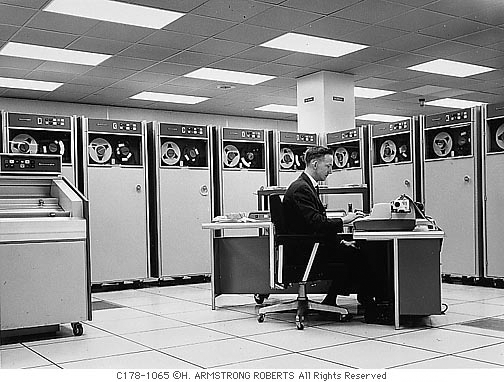
\includegraphics[width=.85\textwidth]{CS1065}}
\caption{Beispiel für einen langen Caption-Text. \textsc{Univac}
brachte 1961 mit dem Modell 751 den ersten Hochleistungsrechner
mit Halbleiterspeicher auf den Markt. Von diesem Computer wurden
in den U.S.A.\ bereits im ersten Produktionsjahr über fünfzig
Exemplare verkauft, vorwiegend an militärische Dienststellen,
Versicherungen und Großbanken. Die Ablöse erfolgte zwei Jahre
später durch das zusammen mit \textsc{Sperry} entwickelte Modell 820.
Das klingt vielleicht plausibel, ist aber frei erfunden und
vermutlich völliger Unsinn.} 
\label{fig:univac}
\end{figure}





\section{Abbildungen}

Für die Einbindung von Grafiken in \latex wird die Verwendung des Stan\-dard-Pakets
\texttt{graphicx}\footcite{Carlisle99} empfohlen 
(wird durch das \texttt{htl}-Paket bereits eingebunden). 
Folgende Bildformate können verwendet werden:
%
\begin{center}
\begin{tabular}{|l|l|l|}
\hline
Rasterbilder:    & PNG, JPEG, PDF \\
\hline
Vektorgraphiken: & PDF \\
\hline
\end{tabular}
\end{center}
%

\subsection{Wo liegen die Grafikdateien?} 

Die Bilder werden üblicherweise in einem Unterverzeichnis (oder in mehreren Unterverzeichnissen) abgelegt,
im Fall dieses Dokuments in \url{images/}.
Dazu dient die folgende Anweisung
am Beginn des Hauptdokuments \url{Diplomarbeit.tex} (\sa\ Anhang
\ref{app:latex}):
%
\begin{quote}\small
\verb!\graphicspath{{images/}}!
\end{quote}
%
Der (zum Hauptdokument relative) Pfad \texttt{graphicspath} kann innerhalb des
Dokuments jederzeit geändert werden, was durchaus nützlich ist, wenn man
\zB\ die Grafiken einzelner Kapitel getrennt in entsprechenden Verzeichnissen
ablegen möchte.
Die Größe der Abbildung im Druck kann durch Vorgabe einer bestimmten
Breite oder Höhe oder eines Skalierungsfaktors gesteuert werden, {\zB}:
%
\begin{quote}\small
\verb!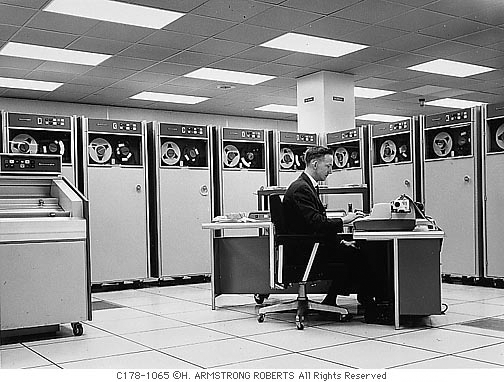
\includegraphics[width=.85\textwidth]{CS1065}! \\
\verb!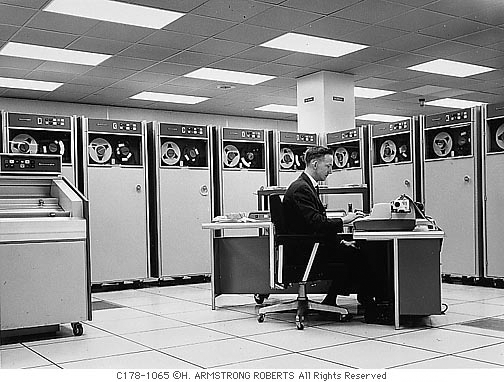
\includegraphics[scale=1.5]{CS1065}!
\end{quote}
%
Man beachte, dass dabei die Datei-Extension nicht explizit angegeben werden muss. 
Das ist \va\ dann praktisch, wenn man verschiedene Workflows mit jeweils
unterschiedlichen Dateitypen verwendet.


\subsection{Grafiken einrahmen} 

Mit dem Makro \verb!\FramePic{}! (definiert in \texttt{htl.sty}) kann man
optional einen dünnen Rahmen rund um die Grafik erzeugen, \zB:
%
\begin{quote}\small
\verb!\FramePic{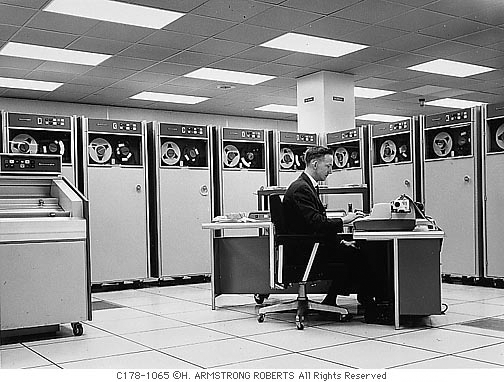
\includegraphics[height=50mm]{CS1065}}!
\end{quote}
%
Das wird man üblicherweise nur bei Rasterbildern tun, insbesondere wenn sie zum Rand hin sehr hell sind
und ohne Rahmen nicht vom Hintergrund abgrenzbar wären.

\subsection{Rasterbilder (Pixelgrafiken)}

Generell sollte man Bilder bereits vorher so aufbereiten,
dass sie später beim Druck möglichst wenig an Qualität verlieren.
Es empfiehlt sich daher, die Bildgröße (Auflösung) bereits im Vorhinein
(\zB mit \emph{Photoshop})
richtig einzustellen.
Brauchbare Auflösungen bezogen auf die endgültige Bildgröße sind:
%
\begin{itemize}
  \item \textbf{Farb- und Grauwertbilder:} 150--300 dpi
  \item \textbf{Binärbilder (Schwarz/Weiß):} 300--600 dpi
\end{itemize}
%
Eine wesentlich höhere Auflösung macht aufgrund der beim Laserdruck notwendigen
Rasterung keinen Sinn, auch bei 1200 dpi-Druckern.
Speziell \emph{Screen\-shots} sollte man nicht zu klein darstellen,
da sie sonst schlecht lesbar sind (max.\ 200 dpi, besser 150 dpi).
Dabei ist zu bedenken, dass die Arbeit auch als Kopie in allen
Details noch gut lesbar sein sollte.

\subsubsection{JPEG-Problematik}

Keinesfalls sollte man Bilder, die für den Einsatz in
Druckdokumenten gedacht sind, mit verlustbehafteten
Kompressionsverfahren abspeichern. Insbesondere sollte man die Verwendung
von JPEG möglichst vermeiden, auch wenn viele Dateien dadurch
wesentlich kleiner würden. 
Eine Ausnahme ist, wenn die Originaldaten nur in JPEG vorliegen und für die 
Einbindung nicht bearbeitet oder verkleinert wurden. Ansonsten sollte man immer
PNG verwenden.

Besonders gerne werden farbige \textbf{Screenshots} einer JPEG-Kompression%
\footnote{Das JPEG-Verfahren ist für natürliche Fotos konzipiert und dafür auch gut geeignet,
seine undifferenzierte Verwendung ist aber zu einer globalen Plage geworden.}
unterzogen, obwohl deren verheerende Folgen auch für jeden Laien sichtbar sein sollten
(Abb.~\ref{fig:jpeg-pfusch}).

\begin{figure}
\centering\small
\begin{tabular}{cc}
\FramePic{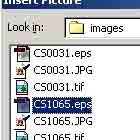
\includegraphics[width=0.45\textwidth]{screenshot-dirty}} &		% JPEG file
\FramePic{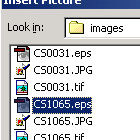
\includegraphics[width=0.45\textwidth]{screenshot-clean}} \\	% PNG file
(a) & (b) 
\end{tabular}
\caption{Typischer JPEG-Pfusch. Screenshots und ähnliche im Original
verfügbare Rasterbilder sollten für Druckdokumente \emph{keinesfalls} mit
JPEG komprimiert werden. Das Ergebnis (a) sieht gegenüber dem
unkomprimierten Original (b) nicht nur schmutzig aus, sondern wird
auch schnell unleserlich.} 
\label{fig:jpeg-pfusch}
\end{figure}






\subsection{Vektorgrafiken}

Für schematische Abbildungen (\zB Flussdiagramme, Entity-Relationship-Diagramme
oder sonstige strukturelle Darstellungen) sollte man unbedingt
Vektorgrafiken verwenden.
Gerasterte Grafiken, wie man sie üblicherweise als GIF- oder PNG-Dateien
auf Webseiten findet, haben in einem Druckdokument nichts zu suchen, notfalls
muss man sie mit einem entsprechenden Werkzeug \emph{neu} zeichnen (natürlich
unter Angabe der ursprünglichen Quelle).

In diesem Fall kommt als Datenformat nur PDF in Frage,
dieses bietet sich aber auch in anderen Umgebungen als universelles
Vektor-Format an.
Zur Erstellung von PDF-Vektorgrafiken benötigt man ein geeignetes
Grafikprogramm, \zB\ \emph{Freehand} von \emph{Macromedia}
oder \emph{Illustrator} von \emph{Adobe}.
Manche gängige Grafikprogramme 
unterstützen allerdings keinen direkten Export von PDF-Dateien
oder erzeugen unbrauchbare Dateien. Vor der Entscheidung
für eine bestimmte Zeichensoftware sollte man das im Zweifelsfall
ausprobieren.
PDF kann im Notfall über einen entsprechenden Druckertreiber erzeugt werden.




\subsubsection{Einbettung von Schriften}

Die Wiedergabe von Textelementen ist abhängig von der auf dem
Computer (oder Drucker) installierten Schriften und der Form der
Schrifteinbettung im Quelldokument. Die korrekte Darstellung am
Bildschirm eines Computers bedeutet nicht, dass dasselbe Dokument
auf einem anderen Computer oder Drucker genau so dargestellt wird.
Dieser Umstand ist besonders wichtig, wenn Druckdokumente online
zur Verfügung gestellt werden. Kontrollieren Sie daher genau, ob
die innerhalb Ihrer Grafiken verwendeten Schriften auch exakt wie
beabsichtigt im Ausdruck aufscheinen.


\subsubsection{Strichstärken -- \emph{Hairlines} vermeiden!}

In Grafik-Programmen wie \emph{Freehand} und \emph{Illustrator},
die sich im Wesentlichen an der \emph{PostScript}-Funktionalität
orientieren, ist es möglich, Linien bzgl.\ ihrer Stärke als
"`Hairline"' zu definieren. Im zugehörigen \emph{PostScript}-Kode
wird dies als \texttt{linewidth} mit dem Wert \texttt{0} ausgedrückt und
sollte am Ausgabegerät "`möglichst dünne"' Linien ergeben. Das
Ergebnis ist ausschließlich vom jeweiligen Drucker
abhängig und somit kaum verhersagbar. 
\textbf{Fazit:} Hairlines vermeiden und stattdessen immer konkrete
Strichstärken ($\geq 0.25 \mathrm{pt}$) einstellen!


\subsection{\tex-Schriften auch in Grafiken?}
\label{sec:tex-schriften-in-grafiken}

Während man sich bei Abbildungen, die mit externen
Grafik-Programmen erzeugt werden, meist mit ähnlich aussehenden
Schriften (wie \emph{Times-Roman} oder \emph{Garamond}) abhilft,
besteht bei Puristen oft der verständliche Wunsch, die 
\emph{Computer-Modern} (CM) Schriftfamilie von {\tex}/{\latex} auch
innerhalb von eingebetteten Grafiken einzusetzen.

\subsubsection{\emph{BaKoMa}-Schriften}

Glücklicherweise stehen einige Portierungen von CM als {\em
TrueType}-Schriften zur Verfügung, die man auch in herkömmlichen
DTP-Anwendungen unter \emph{Windows} und \emph{Mac~OS} verwenden
kann. Empfehlenswert ist \va\ die \emph{BaKoMa Fonts
Collection}\footnote{Von Basil K.\ Malyshev -- die BaKoMa-Fonts
liegen dieser Vorlage bei, ansonsten findet man sie \zB\ unter
\url{www.ctan.org/tex-archive/fonts/cm/ps-type1/bakoma/}.}, die
neben den CM-Standardschriften auch die mathematischen Schriften
der AMS-Familie ent\-hält und zudem kostenfrei ist. Natürlich
müssen die TrueType Schriften vor der Verwendung zunächst auf dem
eigenen PC installiert werden.


\subsection{Abbildungen mit mehreren Elementen}

Werden mehrere Bilder oder Grafiken zu einer Abbildung zusammengefasst, 
verwendet man üblicherweise eine gemeinsame Caption, wie in Abb.~\ref{fig:Bearings}
dargestellt. Im Text könnte ein Verweis auf einen einzelnen Teil der Abbildung, etwa das 
einreihige Rollenlager in Abb.~\ref{fig:Bearings}\thinspace(c), so aussehen:
%
\begin{itemize}
\item[] \verb!Abb.~\ref{fig:Bearings}\thinspace(c)! 
\end{itemize}
%
Für kompliziertere Abbildungen sollte man die Verwendung des 
\texttt{subcaption}-Pakets \footcite{Cochran95} in Betracht ziehen. Ein Beispiel ist in der Vorlage in Abbildung \ref{fig:Settings} zu finden.


\subsection{Quellenangaben in Captions}
\label{sec:QuellenangabenInCaptions}

Wenn Bilder, Grafiken oder Tabellen aus anderen Quellen verwendet werden, dann muss ihre Herkunft in jedem Fall klar ersichtlich gemacht werden, und zwar am besten direkt in der Caption.
Verwendet man beispielsweise eine Grafik aus einem Buch oder einer sonstigen zitierfähigen Publikation, dann sollte man diese in das Literaturverzeichnis aufnehmen und wie üblich zitieren, wie in Abb.\ \ref{fig:Bearings} demonstriert. Da Grafiken floating-Elemente sind, muss statt mit
\verb!\footcite{..}! die Kombination \verb!\footnotemark! und \verb!\footcitetext! verwendet werden. Weitere Details zu dieser Art von Quellenangaben finden sich in Kap.\ \ref{cha:Literatur}.

Bei Bildern aus dem Internet ist es hingegen ratsam, die zugehörige Website \emph{nicht} in das Literaturverzeichnis aufnehmen, sondern (mit \verb!\url{..}!) direkt in der Caption oder in einer Fußnote anzugeben (siehe Abschn.\ \ref{sec:OnlineQuellen} und Abbildung \ref{fig:latexinternet}). 

Sollte die Kombination von Caption, Fußnote und Url verwendet werden, muss die Fußnote in ein \verb!\footnotemark! und ein \verb!\footnotetext! aufgeteilt werden. Abbildung \ref{fig:latexinternet} zeigt ein Beispiel davon und das Programm \ref{prog:footnotemark} zeigt den \latex\ Quelltext. Die Fußnote wird in diesem Fall nicht immer auf der selben Seite wie die Abbildung sein, was durch die Durchnumerierung der Fußnoten jedoch kein Problem darstellen sollte. Vor allem, da die Fußnote sich dann auf der Seite befindet wo die Abbildung im Text erwähnt werden sollte. 

\begin{program}
% place caption consistently either at the top or bottom:
\caption{\latex\ Quelltext zu Abbildung \ref{fig:latexinternet}.}
\label{prog:footnotemark}
%
\begin{LaTeXCode}
\begin{figure}
\centering

\includegraphics[width=.85\textwidth]{LatexInternet}
\caption[]{Witze über Latex im Internet.\footnotemark }
\label{fig:latexinternet}
\end{figure}
\footnotetext{Quelle: \url{https://pr0gramm.com/static/1454890}}
\end{LaTeXCode}
%
\end{program}

% Beispiel für die Verwendung von "subfigure"

\begin{figure}
\centering\small
\begin{tabular}{cc}
  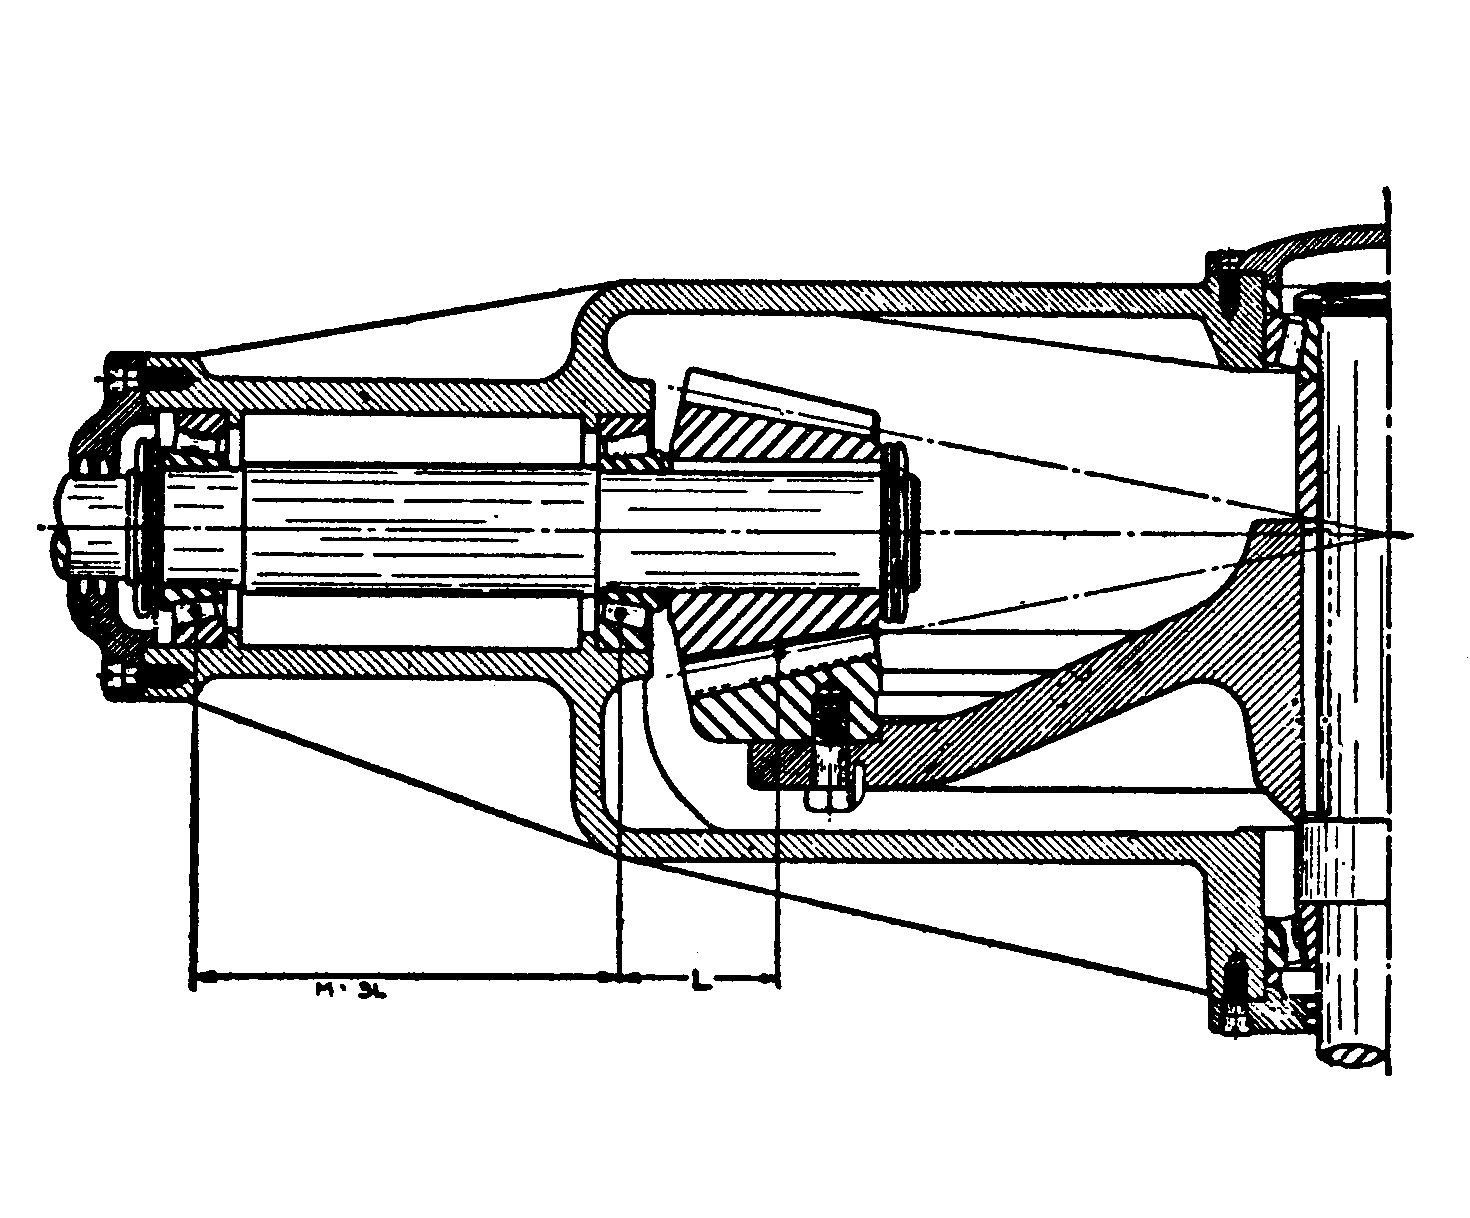
\includegraphics[width=.45\textwidth]{overhang-mounting} &
  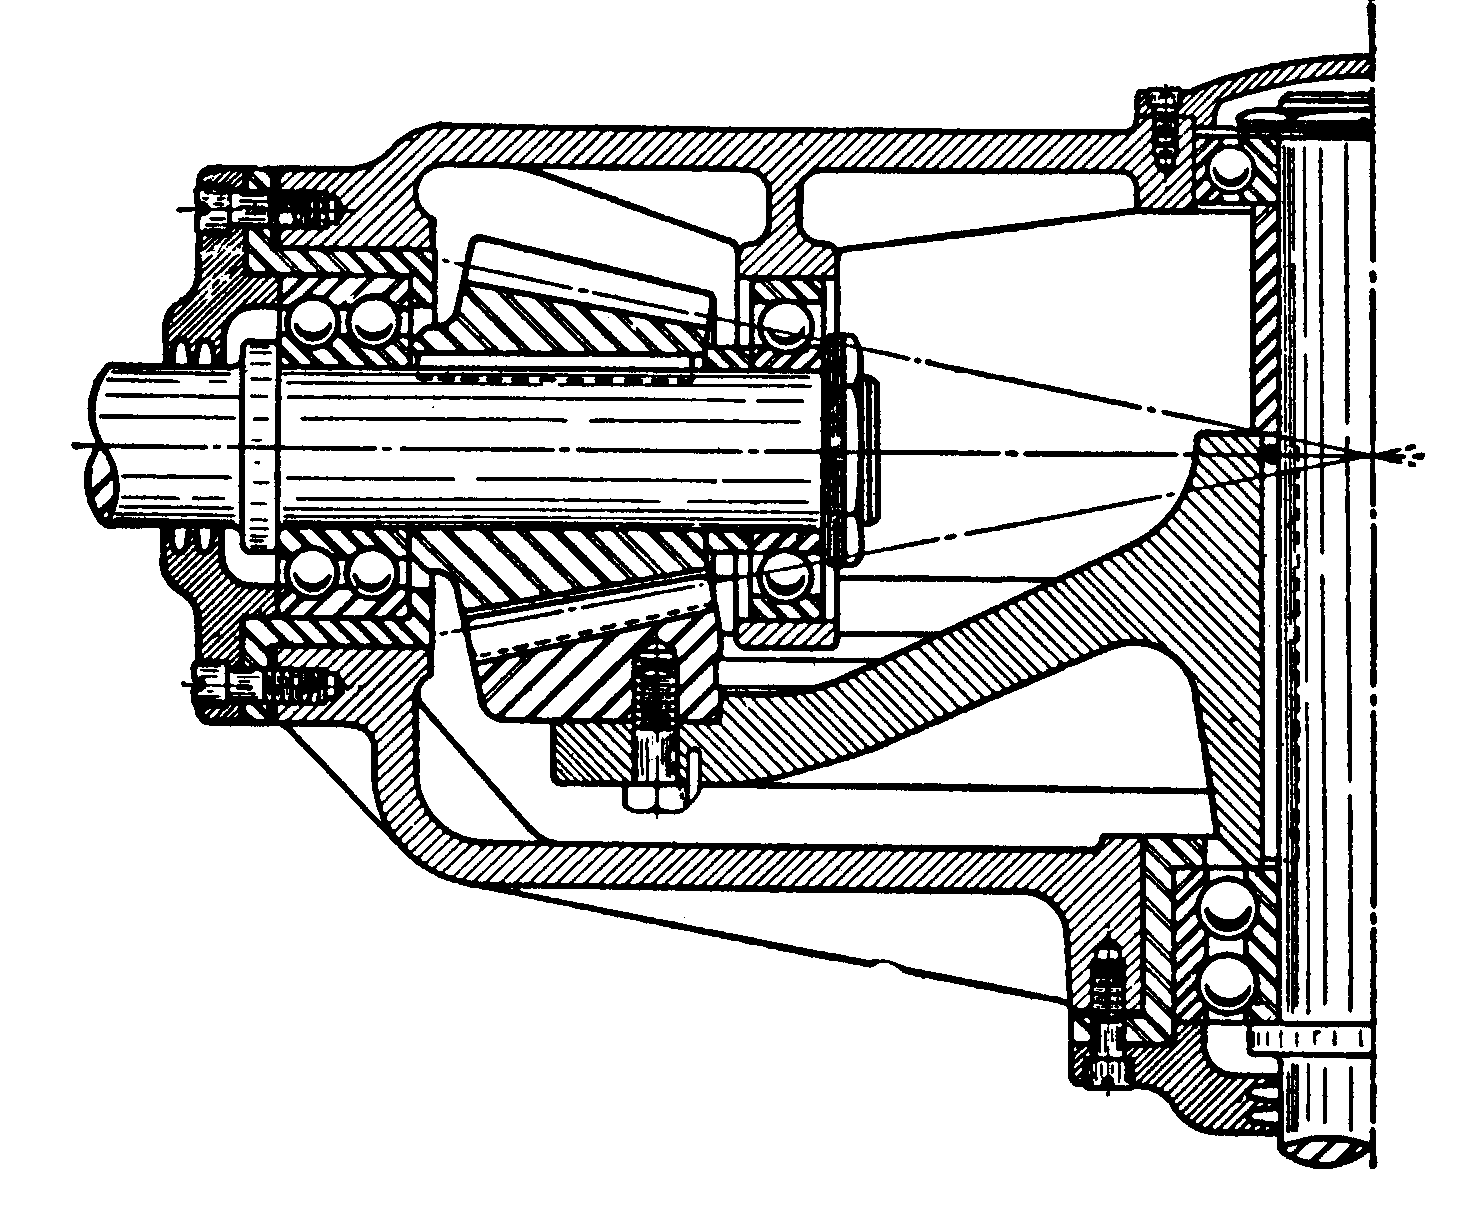
\includegraphics[width=.45\textwidth]{straddle-mounting} \\
  (a) & (b)
\\[4pt]	%vertical extra spacing (4 points)
  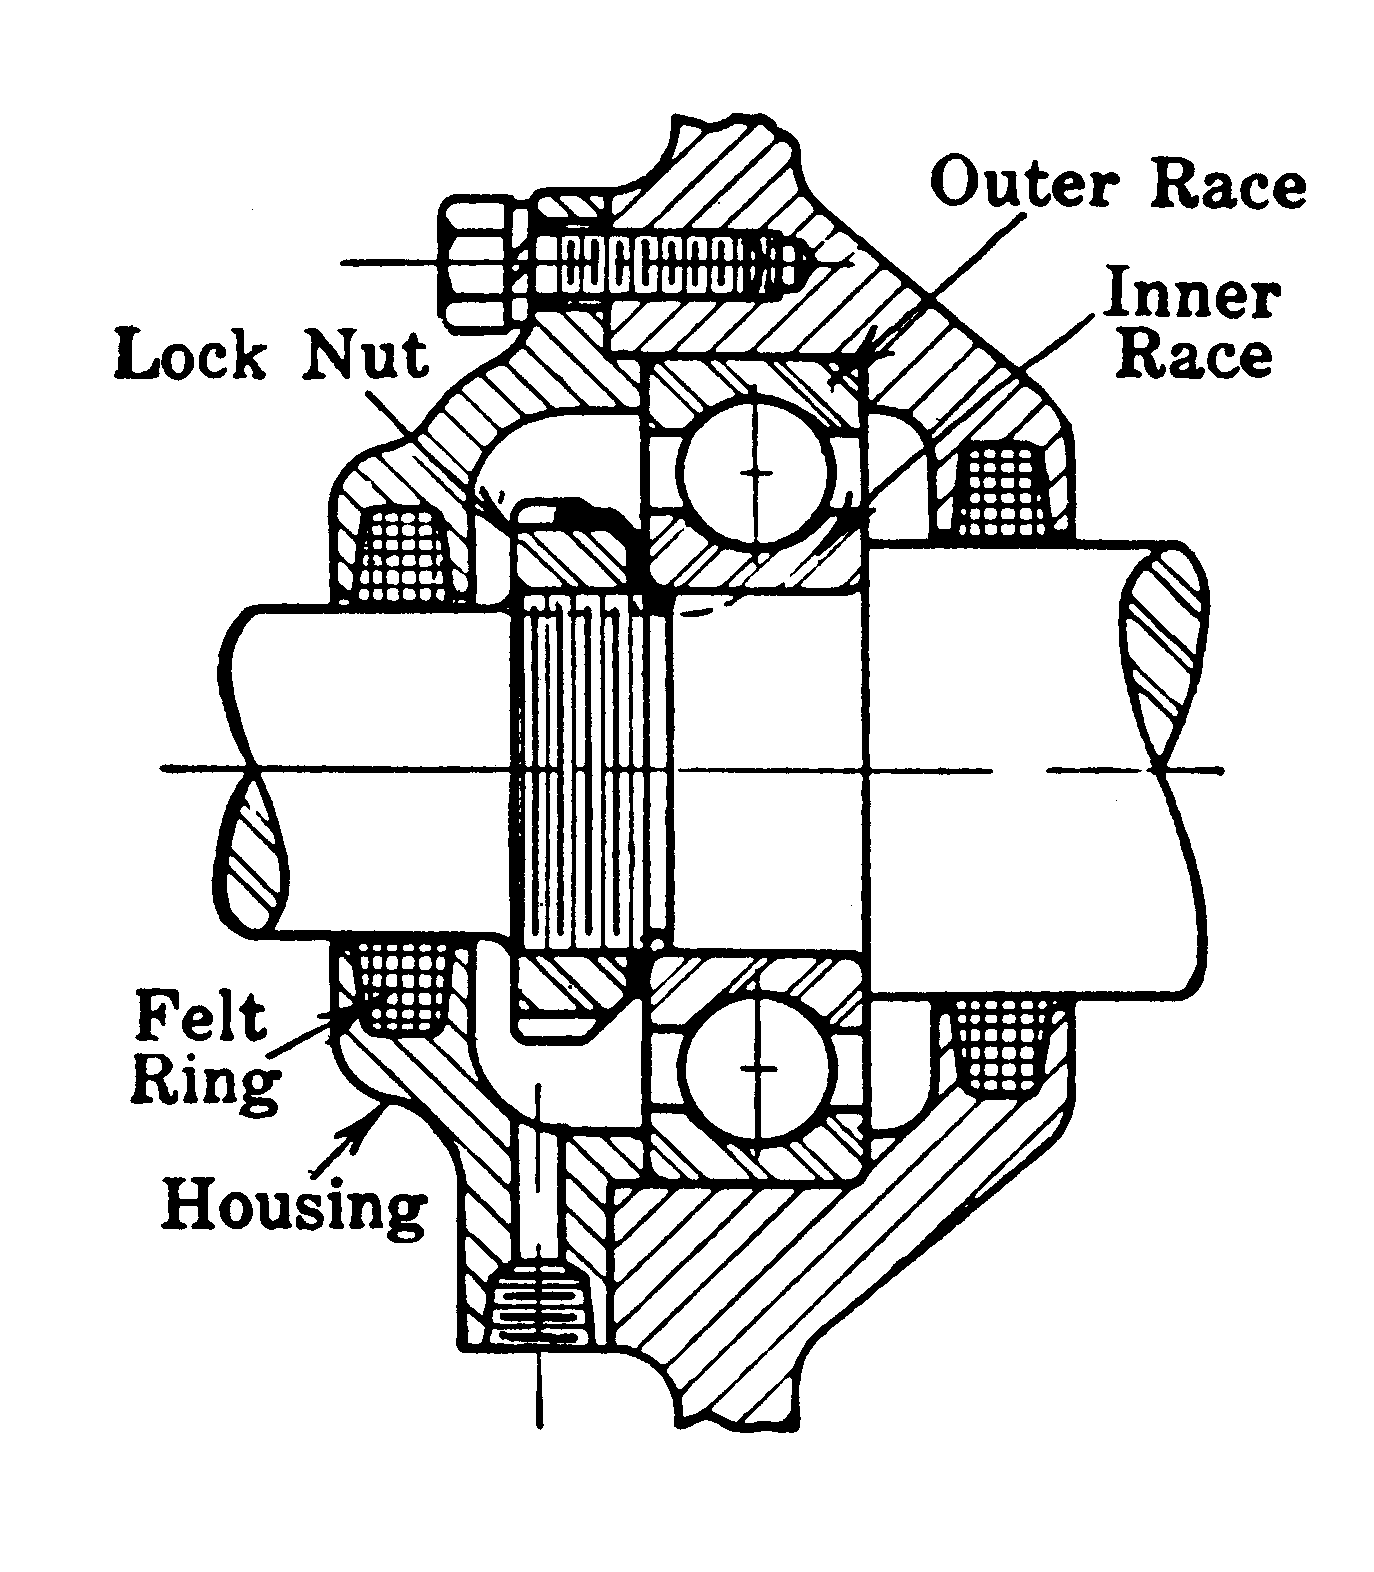
\includegraphics[width=.45\textwidth]{ball-bearing-1} &
  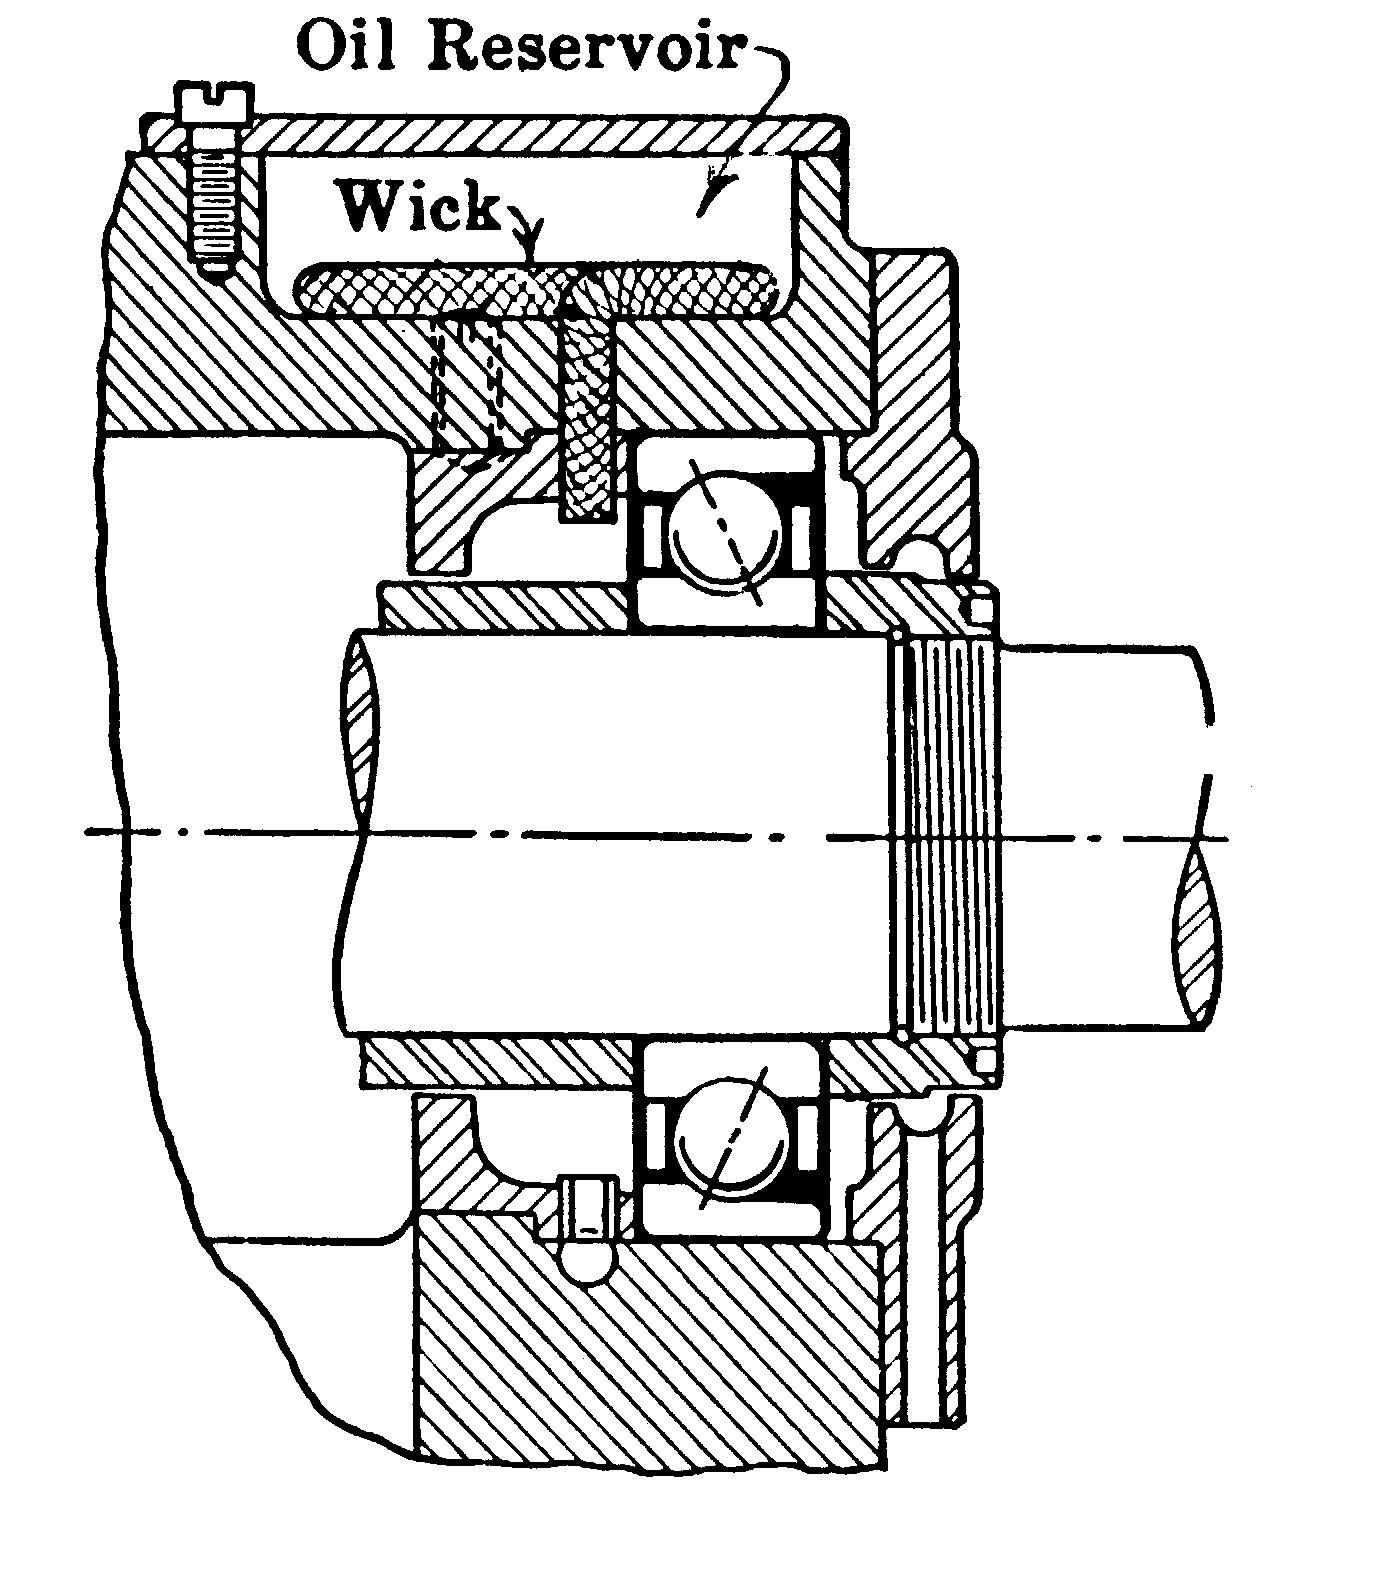
\includegraphics[width=.45\textwidth]{ball-bearing-2} \\
  (c) & (d)
\end{tabular}
%
\caption[]{Diverse Maschinenelemente.
Overhang Mounting (a), Straddle Mounting (b),
einreihiges Rollenlager (c), Schmierung von Rollenlagern (d).
Aus \citetitle{Faires34}.\footnotemark }
\label{fig:Bearings}
\end{figure}
\footcitetext{Faires34}

\begin{figure}
\centering

\includegraphics[width=.85\textwidth]{LatexInternet}
\caption[]{Witze über Latex im Internet.\footnotemark }
\label{fig:latexinternet}
\end{figure}
\footnotetext{Quelle: \url{https://pr0gramm.com/static/1454890}}

\section{Tabellen}

Tabellen werden häufig eingesetzt um numerische Zusammenhänge, Testergebnisse
etc.\ in übersichtlicher Form darzustellen.
Ein einfaches Beispiel ist Tab.~\ref{tab:processors}, der \latex-Quelltext dazu
findet sich in Prog.~\ref{prog:processors-source}.


\begin{table}
\caption{Prozessor-Familien im Überblick.}
\label{tab:processors}
\centering
\setlength{\tabcolsep}{5mm}	% separator between columns
\def\arraystretch{1.25}		% vertical stretch factor
\begin{tabular}{|r||c|c|c|} \hline
& \emph{PowerPC} & \emph{Pentium} & \emph{Athlon} \\
\hline\hline
Manufacturer & Motorola & Intel & AMD \\
\hline
Speed & high & medium & high   \\
\hline
Price & high & high   & medium \\
\hline
\end{tabular}
\end{table}

\begin{program}
% place caption consistently either at the top or bottom:
\caption{\latex\ Quelltext zu Tab.~\ref{tab:processors}.
Die Erzeugung des dargestellten Listings selbst ist in Abschn.\ \ref{sec:programmtexte} beschrieben.}
\label{prog:processors-source}
%
\begin{LaTeXCode}
\begin{table}
\caption{Prozessor-Familien im "Uberblick.}
\label{tab:processors}
\centering
\setlength{\tabcolsep}{5mm}	% separator between columns
\def\arraystretch{1.25}		% vertical stretch factor
\begin{tabular}{|r||c|c|c|} \hline
& \emph{PowerPC} & \emph{Pentium} & \emph{Athlon} \\
\hline\hline
Manufacturer & Motorola & Intel & AMD \\
\hline
Speed & high & medium & high   \\
\hline
Price & high & high   & medium \\
\hline
\end{tabular}
\end{table}
\end{LaTeXCode}
%
\end{program}

Manchmal ist es notwendig, in Tabellen relativ viel Text in engen Spalten
unter zu bringen, wie in Tab.~\ref{tab:synthesis-techniques}. In diesem Fall
ist es sinnvoll, auf den Blocksatz zu verzichten und gleichzeit die
strengen Abteilungsregeln zu lockern. Details dazu finden sich im zugehörigen
\latex-Quelltext.


%--------------------------------------------------------------------------------
% Table with narrow columns
%--------------------------------------------------------------------------------
\begin{table}
\caption{Beispiel für eine Tabelle mit mehrzeiligem Text in engen Spalten.
Hier werden die Zeilen für den Blocksatz zu kurz, daher wird linksbündig
gesetzt (im "`Flattersatz"').}
\label{tab:synthesis-techniques}
\centering
\def\rr{\rightskip=0pt plus1em \spaceskip=.3333em \xspaceskip=.5em\relax}
\setlength{\tabcolsep}{1ex}
\def\arraystretch{1.20}
\setlength{\tabcolsep}{1ex}
\small
\begin{english}
\begin{tabular}{|p{0.2\textwidth}|c|p{0.3\textwidth}|p{0.2\textwidth}|}
\hline
   \multicolumn{1}{|c}{\emph{Method}} &
   \multicolumn{1}{|c}{\emph{Implem.}} &
   \multicolumn{1}{|c}{\emph{Features}} &
   \multicolumn{1}{|c|}{\emph{Status}} \\
\hline\hline
   {\rr polygon shading} &
   SW/HW &
   {\rr flat-shaded polygons} &
   \\
\hline
  {\rr flat shading with z-buffer} &
  SW/HW &
  {\rr depth values} &
  \\
\hline
  {\rr goraud shading with z-buffer} &
  SW/HW &
  {\rr smooth shading, simple fog, point light sources} &
  {\rr SGI entry models} \\
\hline
  {\rr phong shading with z-buffer} &
  SW/HW &
  {\rr highlights} &
  \\
\hline
  {\rr texture mapping with z-buffer} &
  SW/HW &
  {\rr surface textures, simple shadows} &
  {\rr SGI high end, flight simulators} \\
\hline
%  {\rr reflection mapping with z-buffer} &
%  SW/HW &
%  {\rr reflections} &
%  {\rr SGI next generation} \\
%\hline
%  {\rr raytracing} &
%  SW &
%  {\rr refraction, real camera model, area light sources with penumbra, realistic material models} &
%  {\rr common ray\-tracers} \\
%\hline
%  {\rr raytracing + global illumination simulation} &
%  SW &
%  {\rr indirect illumination} &
%  \textit{Radiance} \\
%\hline
%  {\rr raytracing + global illumination simulation + dissipating media} &
%  none &
%  {\rr realistic clouds, scattering, ...} &
%  {\rr research} \\
%\hline
\end{tabular}
\end{english}
\end{table}

%--------------------------------------------------------------------------------



\section{Programmtexte}
\label{sec:programmtexte}

Die Einbindung von Programmtexten (source code) ist eine häufige Notwendigkeit,
\va natürlich bei Arbeiten im Bereich der Informatik.

\subsection{Formatierung von Programmkode}
\label{sec:FormatierungVonProgrammkode}

Es gibt für \latex\ spezielle Pakete zur Darstellung von Programmen, die \ua\
auch die automatische Nummerierung der Zeilen vornehmen. Zu empfehlen ist hier
insbesondere das \texttt{listings2}-Package\footnote{Aktuell noch als
Beta-Version, ist notwendig zur Unterstützung von UTF-8.}. In \texttt{htl.sty}
sind damit folgende Umgebungen definiert:
%
\begin{center}
\begin{tabular}{ll}
C (ANSI):   & \verb!\begin{CCode}       ... \end{CCode}! \\
C++ (ISO):  & \verb!\begin{CppCode}     ... \end{CppCode}! \\
Java:       & \verb!\begin{JavaCode}    ... \end{JavaCode}! \\
\latex:     & \verb!\begin{LaTeXCode}   ... \end{LaTeXCode}! \\
PHP:  		& \verb!\begin{PhpCode}     ... \end{PhpCode}! \\
Python:  	& \verb!\begin{PythonCode}  ... \end{PythonCode}! \\
C\#:  		& \verb!\begin{CSharpCode}  ... \end{CSharpCode}! \\
XML:  		& \verb!\begin{XMLCode}  ... \end{XMLCode}! \\
JavaScript:  		& \verb!\begin{JSCode}  ... \end{JSCode}! \\
Generisch:  & \verb!\begin{GenericCode} ... \end{GenericCode}! 
\end{tabular}
\end{center}
%
Der Quellkode innerhalb dieser Umgebungen wird in der jeweiligen Programmiersprache interpretiert, wobei Kommentare erhalten bleiben. Diese Umgebungen können sowohl alleinstehend (im Fließtext) oder innerhalb von Float-Umgebungen (insbes.\ \texttt{program}) verwendet werden. Im ersten Fall wird der Quelltext auch über Seitengrenzen umgebrochen. Mit \verb!/+! ... \verb!+/! ist eine Escape-Möglichkeit nach \latex\ vorgesehen, die \va\ zum Setzen von Labels für Verweise auf einzelne Programmzeilen nützlich ist, \zB
%
\begin{quote}
\verb!/+ \label{ExampleCodeLabel} +/!
\end{quote}
%
Ein Beispiel mit Java ist in Prog.~\ref{prog:CodeExample} gezeigt, wobei der oben angeführte Label in Zeile \ref{ExampleCodeLabel} steht.
Man beachte, dass innerhalb der Kommentare auch mathematischer Text (wie etwa in Zeile \ref{MathInCode} von Prog.~\ref{prog:CodeExample}) stehen kann.

\begin{program}
% place caption consistently either at the top or bottom:
\caption{Beispiel für die Auflistung von Programmkode als Float-Element.}
\label{prog:CodeExample}
\begin{JavaCode}
import ij.ImagePlus;
import ij.plugin.filter.PlugInFilter;
import ij.process.ImageProcessor;

public class My_Inverter implements PlugInFilter {

  String title = ""; // just to test printing of double quotes

	public int setup (String arg, ImagePlus im) {
		return DOES_8G;	// this plugin accepts 8-bit grayscale images \label{pr:IjSamplePlugin10}
	}

	public void run (ImageProcessor ip) {
		int w = ip.getWidth();	/+ \label{ExampleCodeLabel} +/
		int h = ip.getHeight(); 
		
		/* iterate over all image coordinates */
		for (int u = 0; u < w; u++) { 
			for (int v = 0; v < h; v++) {
				int p = ip.getPixel(u, v); 
				ip.putPixel(u, v, 255-p); // invert: $I'(u,v) \leftarrow 255 - I(u,v)$\label{MathInCode}
			}
		}
	}
			
} // end of class {\tt My\_Inverter}
\end{JavaCode}
%
\end{program}


\subsection{Platzierung von Programmkode}

Da Quelltexte sehr umfangreich werden können, ist diese Aufgabe nicht
immer leicht zu lösen. Abhängig vom Umfang und vom Bezug zum Haupttext
gibt es grundsätzlich vier Möglichkeiten zur Einbindung von Programmtext:
%
\begin{itemize}
\item[a)] im laufenden Text für kurze Programmstücke,
\item[b)] als Float-Element (\texttt{program}) für mittlere Programmtexte bis max.\ eine Seite oder
\item[c)] im Anhang (für lange Programmtexte).
\end{itemize}

\subsubsection{Programmtext im laufenden Text}

Kurze Kodesequenzen kann man ohne weiteres im laufenden Text
einbetten, sofern sie an den gegebenen Stellen von unmittelbarer
Bedeutung sind. Die folgende (rudimentäre) Java-Methode {\tt
extractEmail} sucht nach einer E-Mail Adresse in der Zeichenkette
\texttt{line}:

\medskip
\begin{JavaCode}
static String extractEmail(String line) {
    line = line.trim(); // find the first blank
    int i = line.indexOf(' '); 
    if (i > 0)
        return line.substring(i).trim();
    else
        return null;
}
\end{JavaCode}
\medskip

\noindent
Dieses Kodestück wurde mit 
\begin{quote}
\begin{verbatim}
\begin{JavaCode}
static String extractEmail(String line) {
    line = line.trim(); // find the first blank
    ...
}
\end{JavaCode}
\end{verbatim}
\end{quote}
erstellt (siehe Abschn.\ \ref{sec:FormatierungVonProgrammkode}). In-line Programmstücke sollten maximal einige Zeilen lang sein und nach Möglichkeit nicht durch Seitenumbrüche geteilt werden.
Um auch längere Programmzeilen unterzubringen, empfiehlt es sich, dafür
eine entsprechend kleine Schriftgröße zu wählen (als Standardgröße ist
\texttt{footnotesize} eingestellt). 



\subsubsection{Programmtexte als Float-Elemente}
Sind längere Kodesequenzen notwendig, die in unmittelbarer Nähe des laufenden Texts
stehen müssen, sollte man diese genauso wie andere Abbildungen als Float-Elemente
behandeln. Diese Programmtexte sollten den Umfang von einer Seite nicht übersteigen.
Im Notfall kann man auch bis zu zwei Seiten in aufeinanderfolgende Abbildungen packen,
jeweils mit eigener Caption. In \texttt{htl.sty} ist eine neue Float-Umgebung
\texttt{program} definiert, die analog zu \texttt{table} verwendet wird:
%
\begin{quote}
\begin{verbatim}
\begin{program}
\caption{Der Titel zu diesem Programmstück.}
\label{prog:xyz}
\begin{JSCode}
  document.addEventListener('DOMContentLoaded', Geheim);

  function Geheim () {
    var Passwort = 'Traumtaenzer';
    var Eingabe = window.prompt('Bitte geben Sie das Passwort ein', '');

    if (Eingabe != Passwort) {
        alert('Falsches Passwort!');
    } else {
        location.href = 'geheim.htm';
    }
  }
\end{JSCode}
\end{program}
\end{verbatim}
\end{quote}


%
Wenn man möchte, kann man in diesem Fall die Caption auch unten anbringen (aber konsistent und nicht gemischt).
Natürlich darf man auch hier  nicht mit einer linearen  Abfolge im fertigen
Druckbild rechnen, daher sind Wendungen wie
"`... im  folgenden Programmstück ..."' zu vermeiden und entsprechende Verweise
einzusetzen. Beispiele dafür sind die Programme \ref{prog:processors-source} und \ref{prog:CodeExample}.

\subsubsection{Mehrere Codefragmente zusammenfassen}

Mit dem subprogram-Befehl können nicht nur Bilder, sondern auch Programmcodes zusammengefasst werden wie in den Programmen in \ref{prog:multi} zu sehen ist.

\begin{program}
\caption{Zwei Code Beispiele}
	\label{prog:multi}
  \begin{subprogram}[b]{.5\linewidth}
    \begin{JSCode}
  document.addEventListener('DOMContentLoaded', Geheim);

  function Geheim () {
    var Passwort = 'Traumtaenzer';
    var Eingabe = window.prompt('Bitte geben Sie das Passwort ein', '');

    if (Eingabe != Passwort) {
        alert('Falsches Passwort!');
    } else {
        location.href = 'geheim.htm';
    }
  }
\end{JSCode}
    \caption{JavaScript Code Beispiel}
  \end{subprogram}
  \begin{subprogram}[b]{.5\linewidth}
    \begin{XMLCode}
  <Window x:Class="WpfApplication1.MainWindow"
        xmlns="http://schemas.microsoft.com/winfx/2006/xaml/presentation"
        xmlns:x="http://schemas.microsoft.com/winfx/2006/xaml"
        Title="MainWindow" Height="350" Width="525">
  <Grid>
  </Grid>
</Window>
\end{XMLCode}
\caption{XML Code Beispiel}
  \end{subprogram}
  
\end{program}

\subsubsection{Programmtext im Anhang}

Für längere Programmtexte, speziell wenn sie vollständige
Implementierungen umfassen und im aktuellen Kontext nicht
unmittelbar relevant sind, muss man zur Ablage in einem getrennten
Anhang am Ende des Dokuments greifen. Für Hinweise auf bestimmte
Details kann man entweder kurze Ausschnitte in den laufenden Text
stellen oder mit entsprechenden Seitenverweisen arbeiten. Ein
solches Beispiel ist der \latex-Quellkode in Anhang
\ref{app:latex} (Seite \pageref{app:latex}).%
\footnote{%
Grundsätzlich ist zu überlegen, ob die gedruckte Einbindung der gesamten
Programmtexte einer Implementierung für den Leser überhaupt sinnvoll ist, oder
ob man diese nicht besser elektronisch (auf CD-ROM) beifügt und nur exemplarisch
beschreibt.}

\chapter{Protokoll}
\label{chap:Protokoll}

\chapter{Verwandte Arbeiten}
\label{chap:VerwandteArbeiten}
Im Zuge unserer Recherche zu Multi-Wan Bonding sind wir auf verschiedene bereits existierende Hardware-/ und Software-Lösungen gestoßen, welche wir uns in diesem Kapitel genauer Ansehen werden.
Unterschied zwischen hw und sw. Hw bezahlt man einmal software abonnement hw ist standortgebunden software ist für leute die viel reisen
\section{Hardware-Lösungen}
\subsection{Multi-Wan Bonding Router}
\section{Software-Lösungen}
\subsection{Speedify}
Speedify ist eine Bereits existierende Multi-Wan Bonding Software-Lösung die das benützen von mehreren Internetverbindungen gleichzeitig möglich macht. Es ist auch eine VPN, das heißt die Daten werden verschlüsselt vom Benutzer an einen Server gesendet dieser entschlüsselt sie und sendet sie weiter ans Internet. Wenn der Server die Daten aus dem Internet wieder erhält verschlüsselt er Sie wieder und sendet die Daten an den Benutzer welcher diese dann entschlüsselt und verwenden kann.
Bei Speedify sind nur 2GB an Datenübertragung pro Monat kostenlos, wenn man mehr Datenvolumen benötigt muss man sich für ein kostenpflichtiges Abonnement entscheiden. Es gibt 3 verschiedene Abonnements bei denen sich die Anzahl an Nutzern verändert, je Nutzer kann man Speedify auf bis zu 5 Geräten gleichzeitig nutzen.
\begin{itemize}
    \item Für Einzelpersonen um 9.99 USD inkludiert 1 Benutzerkonto
    \item Für Familien um 14.95 USD mit 5 Benutzerkonten
    \item Für Firmenkunden um 9.99 USD pro Person
\end{itemize}
\  \\
Unsere Lösung ist im gegensatz zu Speedify Open Source und komplett kostenlos. Das einzige das von einem Benutzer benötigt wird, ist ein Server mit einer guten Internetanbindung, sowohl der Upload als auch der Download sind dabei wichtig.
\subsection{OpenVPN}
\chapter{Multi-Wan Bonding Proxy Server}
\label{cha:Server}

\section{Anforderungen des Multi-Wan Bonding fähigen Proxy Servers}
Unser Multi-Wan Bonding Proxy Server ist dafür verantwortlich Datenpakete des Windows Treibers zu Empfangen und zusammen zu führen und Antwortpakete aus dem Internet aufzuteilen um die an den Windows Treiber zurück zu senden. Dafür müssen Probleme gelöst werden:
\\
\begin{enumerate}
    \item Sammeln von IP Paketen von mehreren Absendeadressen für das selbe Ziel.
    \item Aufteilen von IP Paketen aus dem Internet auf mehrere Verbindungen des selben Empfängers.
    \item NAT Anwenden auf eingehende und Ausgehende IP Pakete.
\end{enumerate}
\ \\
Weiters handelt es sich bei unserem Multi-Wan Bonding Proxy Server um einen Endpunkt für die zu bündelnten Internetverbindungen. Aufgeteilte Datenpakete treffen von verschiedenen Verbindungen beim Server ein und werden wieder zu einem einzelnen Datenstrom zusammengeführt. Antworten an unseren Proxy Server werden ebenfalls entsprechend wieder aufgeteilt und an die verschiedenen WAN-Anbindungen des Nutzers gesendet. 
\\\\
Außerdem müssen gewisse Standards von Performance, Stabilität und Ressourcenanforderungen eingehalten werden. Hierbei gilt:
\\
\begin{enumerate}
    \item Maximale prozentuale CPU Auslastung von 5 {\%}, bei einer 100 Mbit/s Übertragungsrate auf einem AMD Ryzen 7 3700X
    \item Nicht mehr als 300 Megabyte RAM bedarf höchstens.
\end{enumerate}

\section{Server Infrastruktur}
\subsection{Betriebssystem}
Wir haben uns bei der Wahl des Server Betriebsystems für Linux entschieden. Um genau zu sein für Debian 8. 
Dafür gibt es einige Gründe:
\\
\begin{enumerate}
    \item Der Linux Kernel besitzt bereits Standardmäßig einen TUN/TAP Treiber was die Entwicklung des Servers um einiges vereinfacht. Bei Windows müsste man erst einen eigenen Treiber schreiben bzw. eine externe Bibliothek verwenden um einen virtuellen Netzwerkadapter zu erstellen. Dies ist unter Linux nicht notwendig.
    \item Mittels iptables ist es nur ein minimaler Aufwand NAT auf einen Netzwerkadapter anzuwenden. 
    \item Debian ist im vergleich zu Windows um einiges "leichter" damit sinken die Leistungsanforderungen an das Hostsystem erheblich. Debian benötigt Beispielsweiße keinen Desktop. Der Proxy Server selbst ist auch sehr Leistungsschonend weshalb hier schon ein älterer Raspberry PI ausreichen würde.
\end{enumerate}
\ \\
Es gibt aber viele Linux distributionen die diese Funktionalitäten haben. Warum haben wir uns also speziell für Debian 8 entschieden? Die beliebtesten Serverbetriebsysteme sind aktuell Debian, Ubuntu, CentOS und Windows ohne spezielle Reinfolge. Die entscheidung viel auf Debian weil es sich nicht nur um eine der am weitesten verbreiteten Distributionen handelt sondern auch weil es viele andere Distributionen gibt die auf Debian aufbauen. Ubuntu ist eine davon. Dies erlaubt es unserem Server auf einer vielzahl an Servern ohne hohem Aufwand zu laufen. Wir sind uns aber ziemlich sicher das es auch unter anderen Linux Distributionen keine großen Probleme geben sollte sofern man den Source-Code extra für diese kompiliert.

\subsection{Hardware}
Die Anforderungen an die Hardware sind minimal. Selbst ein schwaches Hostsystem kann unseren  Proxy Server ohne Probleme betreiben. 1GB Arbeitsspeicher ist mehr als genügend und mit 2GHz CPU Takt sollten bereits höhere Datenübertragungsraten ohne Probleme möglich sein. 
\\\\ 
Die höchste Relevanz für die Leistung unseres Proxy Servers hat die single Core Leistung des Rechners. Besonders wenn Datenraten von über 100Mbit/s das Ziel sind sollte man darauf achten.
\\\\
Die Internetanbindung ist auch von besonders hoher Relevanz. Die Summer aller mit dem Server verbundenen Nutzer kann zusammen nie eine höhere Übertragungsrate als der Hastrechner haben. 
\\\\
Festplattenspeicher wird praktisch keiner benötigt. Schon ein paar MB sind ausreichend um den Server in Betrieb zu nehmen. Vorrausgesetzt es werden keine Logfiles gespeichert.


\section{Kommunikation zwischen Server und Client}
\subsection{Der Weg eines Datenpakets von Client zu Server}
Möchte eine Anwendung etwas aus dem Internet abrufen so sendet diese Datenpakete aus. Diese Datenpakete enthalten jeweils eine Absender IP-Adresse, eine Ziel IP-Adresse, Nutzdaten und weitere Metainformationen. Diese Datenpakete müssen nun ihren weg von der Anwendung bis zum Ziel Server bestreiten. 
\\\\
Dabei werden sie, nachdem sie von der Anwendung an der Betriebsystem übergeben wurden, geroutet. Beim Routing wird für ein Datenpaket anhand der Ziel IP-Adresse ein passender Netzwerkadapter gesucht an, den das Datenpaket übergeben wird. Gibt es keine spezielle Route für diese IP-Adresse wird die sogenante Standard-Route genommen. Die Standard-Route fürt im Normalfall zu einem Router dieser Router betreibt Heutzutage erheblich mehr als nur simples Routing ins Internet. 
\\\\
Praktisch immer ist auf diesen Haushalts-Routern eine NAT Funktion aktiviert. Sollte unser Datenpaket nicht für das lokale Netzwerk bestimmt und damit wieder die Standard-Route angewandt werden muss es hier nun eine NAT Wall durchqueren. Dabei ändert sich die Absender IP-Adresse zur öffentlichen IP-Adresse des Routers bevor das Datenpaket ins Internet weitergeleitet wird. Die Ziel IP-Adresse wird später auf die öffentliche IP-Adresse des Routers Antworten.
\\\\
Um nun mehrere verschiedene Internetverbindungen zu bündeln müssen wir Datenpakete für das selbe Ziel über verschiedene Netzwerkadapter hinaussenden. Dies wird in unserem Fall von unserem Windows Treiber erledigt. Dieser leitet Datenpakete für die Standard-Route zu sich und teilt diese dann auf die physische Netzwerkadapter auf. Aufteilen alleine ist hier aber nicht genug da dann beim Zielrechner zusammengehörende Datenpakete von verschiedenen IP-Adressen ankommen würden. 
\\\\
Normale Server sind für diese Art der Kommunikation nicht ausgelegt. Besonders sehr Session behaftete Dienste sollten hier größe Probleme haben wie FTP. FTP schickt nicht mit jedem Datenpaket mit zu welchem aktuell Verbundenem FTP-Nutzer dieses Datenpaket gehört. Kommt nun ein Datenpaket von einer anderen IP-Adresse und sogar von einem anderen Port hat ein FTP-Server keine möglichkeit festzustellen zu welchem Nutzer diese Daten gehört haben. 
\\\\
Um dieses Problem zu behandeln haben wir einen Multi-Wan Bonding Proxy Server entwickeln müssen. Anstelle die Datenpakete einfach nur auf die Netzwerkadapter aufzuteilen verpackt unser Windows Treiber sie zuvor in eigenen Datenpaketen welche an unseren Proxy Server adressiert sind. Unser Server ist darauf ausgelegt von mehreren verschiedenen IP-Adressen und Ports Datenpakete zu empfanden. 
\\\\
Woher weiß unser Server welches Datenpaket zu welchem Nutzer gehört? Der Windows Treiber hat einen virtuellen Netzwerkadapter dieser virtuelle Netzwerkadapter hat eine IP-Adresse. Diese IP-Adresse können wir verwenden um verschiedene Nutzer zu unterscheiden. Aktuell haben wir aber noch keine explizite Mehrbenutzerfähigkeit eingebaut. Trotzdem ist es zumindest erforderlich das sich die IP-Adresse des virtuellen Netzwerkadapters des Nutzers im selben Subnetz befindet wir die IP-Adresse des virtuellen Netzwerkadapters des Servers. Da sonst die entpackten Datenpakete des Nutzers nicht vom virtuellen Netzwerkadapter des Servers akzeptiert werden.
\\\\
Der Server nimmt die verpackten Datenpakte, entpackt diese, wendet auf sie NAT an um sie  dann mit seiner eigenen IP-Adresse als Absender an die Ziel-Adresse zu versenden.

\subsection{Der Weg eines Datenpakets von Server zu Client}
Sendet ein Zielrechner aus dem Internet eine Antwort auf eine Anfrage unseres Proxy Servers so wird auf diese bei der Ankunft NAT angewendet. Nachdem durchschreiten der NAT Wall erhält das Datenpaket eine neue Ziel-Adresse nämlich jene die beim senden der Anfrage vom Nutzer noch unsere Absederadresse war.
\\\\
Die Absenderadresse war ursprünglich die IP-Adresse des virtuellen Netzwerkadapters unseres Windows Treibers. Anhand dieser Ziel IP-Adresse könnte der Server nun feststellen an welchen Nutzer er das Paket zurück senden muss bzw. dadurch weiters an welche der verschiedenen Eingehenden verbindungen und an welche nicht. Da Multiusersupport aber in dem Prototypen noch nicht enthalten ist wird eine Antwort aktuell einfach auf alle vorhandenen Verbindungen aufgeteilt. Die Empfänger IP-Adresse muss aber trotzdem wieder korrekt gesetzt werden da sonst der virtuelle Netzwerkadapter des Clients das Datenpaket nicht akzeptieren würde.
\\\\
Nach dem durchqueren der NAT Wall werden die Datenpakete nun einfach wieder verpackt und an die Internetadressen und Ports zurück gesendet von denen ursprünglich die Anfrage stammt.
\\\\
Nun landen die Datenpakete wieder beim Router des Nutzers bei diesem wird beim durchqueren der NAT Wall die öffentliche IP-Adresse des Nutzers wieder gegen die lokale IP-Adresse ersetzt und an das Datenpaket an den Rechner des Nutzers gerouted.
\\\\ 
Beim Rechner des Nutzers werden diese Datenpakete nun wieder vom Windows Treiber entpackt und an den virtuellen Netzwerkadapter übergeben, welcher die Datenpakte wiederum an die ursprüngliche Applikation übergibt.


\section{Architektur des Multi-Wan Bonding fähigen Proxy Servers}
\subsection{Sammeln von IP Paketen von verschiedenen Absendern}
Um IP Pakete die von unserem Windows Treiber kommen entgegennehmen zu können lauscht der Proxy Server Standardmäßig auf Port 5555 nach UDP Datagrams. 
\\\\
Jedes dieser Datagrams enthält wiederum ein IP Paket des Windows Treibers als Nutzdaten. Das IP Paket im inneren des Datagrams wird nun genommen und weiter durch den Server verarbeitet.
\\\\
Die Nutzdaten sind aber nicht die einzig Wichtigen Informationen in dem Datagram. Der Server speichert sich auch den Endpunkt von dem das Datagram gekommen ist. Dies ist Notwendig da wir davon ausgehen müssen das eine NAT Wall zwischen dem Windows Treiber und Server ist. Durch eine NAT Wall ändert sich jedoch der Absende Port und die IP Adresse. Um später also Daten auch zurück schicken zu können ist es Notwendig sich Port und IP-Adresse zu merken. Einen fixen Port können wir beim zurückschicken deswegen auch nicht nehmen.
\\\\ 
Rücksicht auf einen eventuell beschädigten Inhalt des Datagrams müssen wir auch nicht nehmen. Um die Fehlerbehandlung kümmert sich das TCP im inneren der Nutzdaten des Datagrams. Tatsächlich wäre es ein Problem TCP und nicht UDP zur übertragung zu verwenden da wir dann meistens TCP Pakete über eine TCP Verbindung senden würden. Dies würde zu einem sogenannten TCP Meltdown führen.

\subsection{Senden der gesammelten IP Pakete des Windows Treibers}
Die Nutzdaten der gesammelten Datagrams sind selbst wieder IP Pakete. Diese nehmen wir nun und übergeben als byte Arrays an den virtuellen Netzwerkadapter. Da Datenpakete betreten den virtuellen Netzwerkadapter hierbei von der selben Seite wie es bei einem physischen Netzwerkadapter die Bits und Bytes über das Patch Kabel würden.
\\\\  
Danach wird das Datenpaket gerouted. In den meisten Fällen wird es wohl ein Paket für das Internet sein es kann aber auch ein Paket für die IP-Adresse den virtuellen Netzwerkadapters des Servers sein oder für die öffentliche IP-Adresse des Servers. Sollte an dem Server noch ein weiteres Netzwerk hängen so kann das Paket auch für dieses sein. Ist es jedoch für das Internet bestimmt wird die Standard Route gewählt welche zu dem Netzwerkadapter ins Internet führt. 
\\\\
Nachdem das Paket nun gerouted wurde kommt es hier vor dem versenden ins Internet noch zur Anwendung von NAT. Der Grund dafür ist das die IP-Adresse des Servers nun vom Server selbst als auch von den Nutzern des Proxy Servers verwendet wird. Wärend diesem NAT Prozess wird die Absender IP-Adresse gegen die öffentliche IP-Adresse des Servers getauscht. Danach verlässt das Datenpaket unseren Server ins Internet.

\subsection{Entgegennehmen von Antwort Paketen aus dem Internet}
Antworten aus dem Internet werden direkt nach dem eintreffen beim Server wieder durch die NAT Wall gezogen. Dabei wird die Ziel IP-Adresse, welche bis zu diesem Punkt die öffentliche IP-Adresse des Servers war, gegen die lokale IP-Adresse des virtuellen Netzwerkadapters des Windows Treibers eingetauscht.
\\\\ 
Nun wird das Datenpaket gerouted. Da das routing Ziel die IP-Adresse des Windows Treiber seinen virtuellen Netzwerkadapter ist wird das Datenpaket an den virtuellen Netzwerkadapter des Servers übergeben. Dies geschied da sich der virtuelle Netzwerkadapter des Servers und des Windows Treibers im selben subnetz befinden müssen.  
\\\\
Nach der entgegenname durch den virtuellen Netzwerkadapter erhalten wir das IP Paket als byte array welches wir nun wieder an den Windows Treiber senden müssen.

\subsection{Senden von Antwort Paketen an den Windows Treiber}
Jene Datenpakete welche wir als Byte Arrays aus dem virtuellen Netzwerkadapter gezogen haben senden wir über die ganz normale UDP Socket API unter Linux an den Windows Treiber. 
\\\\
Dabei erstellen wird wieder ein Datagram und verwenden als Nutzdaten das IP Paket welches wir als byte array vorliegen haben. Als Zieladresse und Ziel Port verwenden wir einen der Endpunkte welche wir beim Empfangen der Anfragen erhalten haben.
\\\\
Nun durchqueren das Datagram vermutlich noch die NAT Wall des Nutzers bevor es vom Windows Treiber weiter verarbeitet wird. 


\section{Implementierung des Multi-Wan Bonding Proxy Servers}
\subsection{Notwendigkeit eines virtuellen Netzwerkadapters}
Zur implementierung unseres Multi-Wan Bonding Servers ist ein virtueller Netzwerkadapter notwendig. Der Grund dafür ist das es für uns keine andere möglichkeit gibt Datenpakete in ihrer roh Form, in unserem Fall byte arrays, von dem System zu bekommen oder zu übergeben. 
\\\\
Anwendungen verwenden für gewöhnlich entsprechende "System Calls" um die Netzwerk Funktionalitäten des Betriebsystems zu verwenden. Anders würde es auch nicht gut gehen da Anwendungen die direkt mit der Hardware kommunizieren ein Sicherheitsrisiko darstellen würden.
\\\\
Natürlich wäre es für uns auch möglich gewesen eine eigene API ohne virtuellen Netzwerkadapter zu erstellen, dies würde jedoch dazu führen das NetShare nur von jenen Applikationen verwendet werden könnte die unsere API implementieren. Um nun von allen Arten von Applikationen Datenpakete zu erhalten ist es also Notwendig die selben Netzwerkschnittstellen zu verwenden wie es auch eben jene Applikationen tun.  
\\\\
Zwar müssen wir nur bei unserem Windows Treiber auf fremd Anwendungen achten aber auch bei unserem Proxy Server bringt uns dieses vorgehen einige Vorteile. Wir müssten Beispielsweiße NAT selbst implementieren. Da wir jedoch einen virtuellen Netzwerkadapter auch auf der Seite des Servers verwenden, können wir von bereits vorhandenen Implementierungen NATs gebrauch machen. Weiters eröffnet uns dies die Möglichkeit den Server einfach mit bereits vorhandener Netzwerksoftware zu erweitern, wie Beispielsweiße um eine Firewall.
\subsection{Treiber für virtuelle Netzwerkkarten im Linux Kernel}
Der Linux-Kernel enthält Standardmäßig einen sogenannten TUN/TAP Treiber. Dieser TUN/TAP Treiber erlaubt es "User Space" Programmen Zugriff auf rohe Netzwerkübertragungen zu nehmen. Dies ist der Fall da es einem ermöglicht wird virtuelle TUN/TAP Netzwerkadapter zu erstellen.
Virtuell bedeutet in diesem Fall das die erzeugten Netzwerkadapter nicht, wie gewöhnlich, physische Hardwaregeräte im Rechner sind, sondern nur virtuell im Kernel existieren. Sie besitzen somit keine physische Komponente. Abseits davon gibt es aber keinen unterschied zu einem physischen Adapter, es können wie gewohnt IP-Adressen, Subnetz etc konfiguriert werden.
\\\\
Dies bedeutet das Übertragungen die den virtuellen Adapter betreten nicht wie gewöhnlich als bits und bytes über ein Kabel, Funk oder ähnliches übertragen werden. Sondern stattdessen werden die Daten einer Anwendung als Bytestream zur Verfügung gestellt. Die Anwendung bekommt dabei einen "File descriptor" von diesem "File descriptor" kann die Anwendung sowohl lesen als auch schreiben. Es gilt dabei jedoch zu beachten das man nicht beliebige dinge in den Adapter schreiben kann, es muss sich entsprechend formatierte Pakete oder Frames handeln. Für das Betriebsystem selbst sieht es so aus als würde der Adapter wie gewöhnlich per Funk oder Kabel seine Daten lesen/schreiben.
\\\\
Es gibt bei TUN/TAP 2 Grundlegend unterschiedliche Modi. Der Unterschied besteht darin was wir am Ende von dem Adapter lesen beziehungsweise schreiben können. Die 2 Modi werden vom Namen schon angedeutet. Es gibt den TUN Modus und den TAP Modus. Mit welchem dieser beiden Modi der Netzwerkadapter am Ende arbeitet wird mittels eines Flags beim erstellen des Adapters festgelegt.
\\
\begin{description}
    \item[TAP - Netzwerk-Wasserhahn] TAP steht im Englischen für Wasserhahn und circa genau so Arbeitet auch ein TAP Gerät.
    Ein virtueller Netzwerkadapter der auf TAP Konfiguriert ist agiert auf OSI Schicht 2. 
    Beim lesen von dem virtuellen Adapter werden nur vollständige Ethernet-Frames gelesen und beim schreiben werden entsprechend auch nur vollständige Ethernet-Frames akzeptiert.
    \\
    \item[TUN - Netzwerk-Tunnel] TUN steht nicht wie TAP für einen Englischen Begriff sondern ist nur eine Abkürzung für Netzwerktunnel. 
    Ist ein virtueller Netzwerkadapter auf TUN konfiguriert Arbeitet er im gegensatz zu TAP nicht auf Schicht 2 sondern auf Schicht 3. Das bedeutet das er beim lesen nur vollständige IP-Pakete anbietet aber auch nicht mehr. Wärend er beim schreiben auch nur vollständige IP-Pakete akzeptiert. 
\end{description}
\

\subsubsection{Lebensdauer eines TUN/TAP Geräts}
Es TUN/TAP Gerät kann für 2 verschiedene Arten von Lebensdauer erstellt werden. Dabei gibt es eine kurzlebige variante und eine langlebige Variante. Die kurzlebige Variante heißt "transient" und die langlebige "persistent".
\\
\begin{description}
    \item[Transient] Ein Netzwerkadapter der "transient" ist wird von dem selben Prozess erstellt und auch gelöscht. Spätestens wenn sich der besitzende Prozess beendet wird auch der virtuelle Adapter zerstört.
    \item[Persistent] Ein virtueller Adapter der "persistent" ist ist wie der name schon sagt langlebig und existiert auch nach beenden des erstellendem Prozesses noch. Andere Prozesse können sich dann später mit dem Adapter verbinden und ihn verwenden. Damit der virtuelle Netzwerkadapter verschwindet muss er explizit gelöscht werden.
\end{description}

\subsubsection{Erstellen und verwalten eines TUN/TAP Geräts}
Um eine virtuelles TUN/TAP Gerät zu erstellen ist es notwendig die entsprechenden Rechte zu besitzen. Traditionelle UNIX Implementierungen unterscheiden grundsätzlich zwischen zwei Arten von Prozessen. Privilegierte Prozesse und unprivilegierte Prozesse. Die effektive UID eines privilegierten Prozesses ist immer 0 was bedeutet das er mit root Rechten gestartet wurde. Privilegierte Prozesse umgehen alle Berechtigungsüberprüfungen des Betriebsystems. 
\\\\
Seit Linux Kernel 2.2 wurden die Berechtigungen die sonst nur einem privilegiertem Prozess zur verfügung stehen weiter in einzelne Berechtigungen verfeinert. Die einzelnen Berechtigungen haben den Namen "Capabilities" und können auf einer per Thread Basis vergeben werden.
\\\\
Insgesamt gibt es 42 dieser Capabilities aber für das erstellen eines virtuellen Netzwerkadapters wird nur eine davon benötigt, nämlich \textbf{CAP\_NET\_ADMIN}. Diese Fähigkeit (Capability) erlaubt es einem Thread, neben dem erstellen eines virtuellen Adapters auch noch:
\\
\begin{enumerate}
    \item Netzwerkadapter zu konfigurieren
    \item Die Administration einer IP Firewall
    \item Die Routing Tabelle zu bearbeiten
    \item Sich an jede IP Adresse zu binden
    \item Den TOS (Type of Service) zu setzen 
    \item Treiber Statistiken zu bereinigen
    \item Einen Adapter in den "promiscuous mode" zu setzen
    \item Multicasting zu aktivieren
    \item Einige Socketoptionen zu setzen
\end{enumerate} 
% https://man7.org/linux/man-pages/man7/capabilities.7.html 
% https://backreference.org/2010/03/26/tuntap-interface-tutorial/
\ \\
Um nun tatsächlich ein TUN/TAP Gerät zu erstellen müssen wir zuerst auf das sogenante \textbf{clone device} zugreifen. Dieses befindet sich Standardmäßig unter \textbf{/dev/net/tun}.
\\\\
Dafür holen wir uns zuerst mit dem \textbf{open(\dq/dev/net/\dq, O\_RDWR);} Systemaufruf einen Dateideskriptor. Jetzt können wir mittels \textbf{ioctl(fd, TUNSETIFF, (void *) \&ifr);} Systemaufruf einen neuen Adapter erstellen.
\\\\
Der ioctl() Systemaufruf erlaubt es IO Geräte zu steuern. Dies geschieht indem unterliegende Geräte parameter manipuliert werden. Übergeben werden in unserem speziellen Fall zuerst der Dateideskriptor, dann die Konstante TUNSETIFF und zuguterletzt ein Zeiger zu einem ifreq struct das folgendermaßen aufgebaut ist:

\begin{program}[H]
    \begin{CppCode}
        struct ifreq {
            char ifr_name[IFNAMSIZ]; /* Interface name */
            union {
                struct sockaddr ifr_addr;
                struct sockaddr ifr_dstaddr;
                struct sockaddr ifr_broadaddr;
                struct sockaddr ifr_netmask;
                struct sockaddr ifr_hwaddr;
                short           ifr_flags;
                int             ifr_ifindex;
                int             ifr_metric;
                int             ifr_mtu;
                struct ifmap    ifr_map;
                char            ifr_slave[IFNAMSIZ];
                char            ifr_newname[IFNAMSIZ];
                char           *ifr_data;
            };
        };
    \end{CppCode}
\end{program}
\noindent
% https://man7.org/linux/man-pages/man7/netdevice.7.html
Die einzigen Felder die für uns beim erstellen relevant sind, sind ifr\_flags und ifr\_name. Bei ifr\_name Handelt es sich um den Namen des Netzwerkadapters welcher auch später bei ifconfig angezeigt wird. Wird kein Name angegeben wird ein generischer Name aller tun0 oder tap20 gewählt. Wärend ifr\_flags definiert ob es sich um ein TUN oder ein TAP Gerät handelt. Da es bei unserem Multi-Wan Proxy Server keinen Grund gibt Schicht 2 Protokolle wie ARP etc zu unterstützen, verwenden kein TAP Gerät sondern ein TUN Gerät welches nur IP-Pakete überträgt. 
\\\\ 
Wird unser ioctl() Systemaufruf erfolgreich abgeschlossen dann wurde der virtuelle Netzwerkadapter erstellt und der Dateideskriptor den wir zuvor erhalten haben kann nun verwendet werden um damit zu Kommunizieren. Hier vollständiger Beispielcode zum anlegen eines virtuellen Adapters:
\begin{program}[H]
    \begin{CppCode}
        #include <linux /if.h>
        #include <linux /if_tun.h>
        
        int tun_alloc(char *dev, int flags) {
          struct ifreq ifr;
          int fd;
          int error_code;
          char *clone_dev = "/dev/net/tun";
        
           /* Holen des Dateideskriptor vom clone device */
           if( (fd = open(clone_dev, O_RDWR)) < 0 ) {
             return fd;
           }
        
           /* Löscht alles an Inhalt aus dem struct */
           memset(&ifr, 0, sizeof(ifr));
        
           /* Das flag ist entweder IFF_TUN oder IFF_TAP
            * wobei auch noch IFF_NO_PI dazu geodert 
            * werden kann um Paket Informatioenn zu 
            * unterdrücken.
            */
           ifr.ifr_flags = flags;   
        
           /* Kopieren des Namen in das struct Fals angegeben */
           if (*dev) {
             strncpy(ifr.ifr_name, dev, IFNAMSIZ);
           }
        
           /* Hier wird dann versucht den Adapter zu erstellen */
           if( (error_code = ioctl(fd, TUNSETIFF, (void *) &ifr)) < 0 ) {
             close(fd);
             return error_code;
           }
        
          /* Nachdem das Gerät erstellt wurde wird nun
           * der Name aus dem struct kopiert. Dies ist 
           * Notwendig für die Situation in der kein Name
           * angegeben wurde. Desswegen muss auch immer 
           * ein Speicherbereich für den dev Zeiger 
           * übergeben werden.
           */
          strcpy(dev, ifr.ifr_name);
        
          /* Am Ende geben wir nur mehr den Dateideskriptor zurück 
           * den wir von nun an für alle weitere Kommunikation
           * mit dem Adapter verwenden.
           */
          return fd;
        }
    \end{CppCode}
\end{program}
\noindent
Der Adapter ist jetzt aber noch nicht persistent sonder erstmal nur transient. Um dies zu ändern erfordert es einige weitere ioctl() Aufrufe. Wir könnten den Adapter in diesen zustand aber schon ohne Probleme verwenden.
\\\\
Um das Netzwerkinterface jetzt auch noch persistent zu machen werden im normalfall zwei ioctl() Systemaufrufe gemacht. Mit dem ersten Aufruf machen wir des Netzwerkgerät tatsächlich schon persistent. Jedoch reicht das oft noch nicht. Der Code zum erstellen und zum einhängen in einen bereits vorhandenen Netzwerkadapter ist identisch, das bedeutet aber auch das die Berechtigungen identisch sein müssen. Wir wollen den Multi-Wan Bonding Proxy Server aber nicht immer mit root Berechtigungen laufen lassen da dies ein mögliches Sicherheitsrisiko darstellt. Die änderung des Besitzers und der Persistenz muss aber noch mit root Rechten erfolgen.
\\\\
Hier kommt uns der zweite ioctl() Aufruf zur Hilfe, dieser erlaubt es uns den Besitzer des virtuellen Netzwerkadapters zu einem nicht root Nutzer zu ändern, was es diesem ermöglicht zugriff zu nehmen. Zum löschen des Netzwerkadapters reicht es aus den Adapter wieder transient zu machen und den Prozess zu beenden. Hier Beispielcode zur Persistentmachung eines virtuellen Netzwerkadapters:
\begin{program}[H]
    \begin{CppCode}
        if(ioctl(tap_fd, TUNSETPERSIST, 1) < 0){
            perror("enabeling TUNSETPERSIST");
            exit(1);
        }
        
        int owner{1002}; // UID des neuen Besitzers
        if(ioctl(tap_fd, TUNSETOWNER, owner) < 0){
            perror("TUNSETOWNER");
            exit(1);
        }

        // Loeschen eines virtuellen Netzwerkadapters
        if(ioctl(tap_fd, TUNSETPERSIST, 0) < 0){
            perror("disabling TUNSETPERSIST");
        }
        exit(0);
    \end{CppCode}
\end{program}
\noindent
Ein Prozess der nun mit der effektiven UID des Adapterbesitzers läuft kann nun mit dem selben Code mit dem normal ein virtueller Netzwerkadapter erstellt wird diesen einhängen. Dabei ist zu beachten das dazu versucht werden muss einen Netzwerkadapter mit genau demselben Namen zu erstellen, wie der für den wir Rechte bekommen haben hat. Generell sollte man versuchen einen weiteren Adapter mit dem selben Namen zu erstellen wir der bereits existierende einfach nur eingehangen sofern man ausreichende Berechtigungen hat.

\subsubsection{Lesen und schreiben von einem TUN/TAP Gerät}
Zum lesen und schreiben verwenden wir einfach den read() und write() Systemaufruf. Diese werden für das Lesen und schreiben von praktisch alles Geräten und Datein verwendet. 
\\
\begin{description}
    \item[read() - Systemaufruf] Bei read() werden drei Parameter übergeben. Zuerst der Dateideskriptor von dem wir lesen möchten, dann ein Zeiger auf einen char Array Buffer und zuguterletzt die Anzahl der zu lesenden Bytes. read() blockiert bis die gewünschte Anzahl an Bytes in den Buffer gelesen wurde oder wir an das Dateiende kommen beziehungsweise bis es zu einem Fehler kommt. Ist read() erfolgreich wird die Anzahl an gelesenen Bytes zurückgegeben, im Fehlerfall wird ein Fehlercode kleiner 0 zurückgegeben.
    \\% https://man7.org/linux/man-pages/man2/read.2.html
    \item[write() - Systemaufruf] Es werden dabei wie auch bei read() der Dateideskriptor, char array Zeiger und größe übergeben. write() blockiert solange bis die Anzahl an bytes per größe übergeben aus dem char array gelesen und in die Datei geschrieben wurden oder ein größen limit der Datei erreicht wurde. Sollte es zu einem Fehler kommen wird auch hier eine Zahl kleiner 0 zurückgegeben, sonst wird die Anzahl der geschriebenen Bytes zurückgegeben.
    % https://man7.org/linux/man-pages/man2/write.2.html
\end{description}
\ \\
Da wir vermeiden möchten Datenpakete zu halbieren oder zumindest nicht vollständig zu lesen und zu schreiben. Müssen wir rücksicht auf die Maximum transmission unit (MTU) des virtuellen Netzwerkadapters nehmen. Die MTU beschreibt die größe der größten möglichen Protokoll Daten Einheit und steht in Verbindung zu der maximalen Frame größe die auf OSI Schicht 2 übertragen werden kann. Bei Ethernet beträgt die MTU 1500 Bytes vorrausgesetzt Jumboframes sind nicht aktiviert was bei unserem virtuellen Adapter nicht der Fall ist.
\\\\
Wir schreiben und lesen von unserem virtuellen Netzwerkadapter also immer maximal 1500 Bytes so können wir sicher gehen das wir immer vollständige Datenpakete entgegennehmen und schreiben.
\\\\
Physisch könnte man sich das nachfolgende Beispiel so vorstellen als hätte man in einem Rechner zwei Ethernet Netzwerkadapter und würde beide mit einem Patchkabel miteinander verbinden. Es ist zwar nicht besonders sinnvoll dies zu tun aber wir können so gut zeigen wie das schreiben und lesen von einem virtuellen Adapter funktioniert. Im Beispiel wird auch ein select() Systemaufruf verwendet um zu überprüfen ob in einem der beiden virtuellen Netzwerkadaptern gerade Datenpakete verfügbar sind und nur dann wird versucht zu lesen. 
\begin{program}[H]
    \begin{CppCode}
        char tun_name1[IFNAMSIZ];
        char tun_name2[IFNAMSIZ];
        char* buffer = new char[1500]; /* MTU größe */
        int tun_fd1, tun_fd2;
  
        /* Erstellen oder einhängen des TUN Adapters */
        strcpy(tun_name1, "tun1");
        tun_fd1 = tun_alloc(tun_name1, IFF_TUN | IFF_NO_PI);

        /* Erstellen oder einhängen des zweiten TUN Adapters */
        strcpy(tun_name2, "tun2");
        tun_fd2 = tun_alloc(tun_name2, IFF_TUN | IFF_NO_PI);
      
        if(tun_fd1 < 0 || tun_fd2 < 0){
          perror("Fehler beim erstellen/einhängen.");
          exit(1);
        }
      
        /* Daten lesen und schreiben. */
        uint16_t nread, nwrite;
        int maxfd = (tun_fd1 > tun_fd12) ? tun_fd1 : tun_fd2;
        while(1) {
            int ret;
            fd_set rd_set;
        
            FD_ZERO(&rd_set);
            FD_SET(tun_fd1, &rd_set); FD_SET(tun_fd2, &rd_set);

            /* Warten auf änderungen bei einem der beiden Dateideskriptoren */
            ret = select(maxfd + 1, &rd_set, nullptr, nullptr, nullptr);
        
            if (ret < 0 && errno == EINTR) {
              continue;
            }
        
            if (ret < 0) {
              perror("select()");
              exit(1);
            }

            // Lesen von tun1 und schreiben in tun2 wenn Inhalt in tun1
            if(FD_ISSET(tun_fd1, &rd_set)) {
                nread = read(tun_fd1, buffer, sizeof(buffer));
                if(nread < 0) {
                    perror("Lesen vom Interface");
                    close(tun_fd1); close(tun_fd2);
                    exit(1);
                }
                printf("Gelesen %d bytes von Gerät %s\n", nread, tun_name1);

                nwrite = write(tun_fd2, buffer, nread);
                if(nwrite < 0) {
                    perror("Schreiben zum Interface");
                    close(tun_fd1); close(tun_fd2);
                    exit(1);
                }
                printf("Geschrieben %d bytes in Gerät %s\n", nwrite, tun_name2);
            }
    \end{CppCode}
\end{program}
\noindent
\begin{program}[H]
    \begin{CppCode}
        // Lesen von tun2 und schreiben in tun1 wenn Inhalt in tun2
        if(FD_ISSET(tun_fd2, &rd_set)) {
            nread = read(tun_fd2, buffer, sizeof(buffer));
            if(nread < 0) {
                perror("Lesen vom Interface");
                close(tun_fd1); close(tun_fd2);
                exit(1);
            }
            printf("Gelesen %d bytes von Gerät %s\n", nread, tun_name2);

            nwrite = write(tun_fd1, buffer, nread);
            if(nwrite < 0) {
                perror("Schreiben zum Interface");
                close(tun_fd1); close(tun_fd2);
                exit(1);
            }
            printf("Geschrieben %d bytes in Gerät %s\n", nwrite, tun_name1);
        }
    }
    \end{CppCode}
\end{program}
\noindent
\subsection{Kommunikation mit unserem Multi-Wan Bonding Windows-Treiber}
Zur Kommunikation zwischen dem Proxy Server und dem Windows Treiber verwenden wir die normale Linux Socket API. Wir setzen hier auf UDP Datagrams. Wie wir schon im vorherigen Abschnitt über den TUN/TAP Treiber lernen konnten sind die größten IP-Pakete mit denen wir rechnen müssen 1500 Bytes groß. Bei der Kommunikation zwischen Server und Windows Treiber machen wir nun nichts anderes als ein UDP Datagram zu verschicken welches als Nutzdaten das IP-Paket enthält welches wir von dem TUN Interface bekommen haben. Genauso läuft es auch in die andere Richtung. Empfangen wir ein UDP Datagram bei unserem Server nehmen wir einfach die Nutzdaten und übergeben sie mit einem write() Systemaufruf an das TUN Interface. Dabei ist uns egal von wo dieses UDP Datagram ursprünglich herkommt. Es werden einfach alle eingehenden Datagrams auf Port 5555 genommen und deren Nutzdaten an den virtuellen Netzwerkadapter übergeben ohne weitere verarbeitungsschritte dazwischen. 
\\\\
Der Port und die IP-Adresse des Absenders des Datagrams wird in einem Set zwischengespeichert. 
\chapter{Treiber}
\label{chap:Treiber}

\chapter{Windows Desktop-Anwendung zur Steuerung des Treibers}
\label{chap:WindowsDesktop-AnwendungzurSteuerungdesTreibers}

%Setzen der Schriftgröße für die Code-Beispiele von Manuel
\lstset{basicstyle=\normalsize}

Um unseren Treiber einfach bedienen zu können, haben wir eine grafische Benutzeroberfläche, kurz GUI, entwickelt. Durch ein simples und intuitives Design ermöglicht unsere Desktop-Anwendung das Verbinden mit einem Server, das Einsehen der aktuellen Netzgeschwindigkeit, sowie das Tätigen von Einstellungen mit nur wenigen Mausklicks. 
\\ \ \\
Anhand der in Kapitel 3.1.3 beschriebenen Vor-und Nachteile haben wir uns dazu entschieden, unsere grafische Benutzeroberfläche mit Windows Forms zu programmieren.
Das GUI-Framework WPF bietet zwar eine größere Freiheit im Bezug auf das Designen, aber dadurch kann das Implementieren auch schnell unnötig kompliziert und aufwändig werden. Das Problem, das man bei der Auswahl der Elemente auf die Standard-Windows-Benutzerelemente beschränkt ist, kann mit einigen Tricks umgangen werden, sodass auch in WinForms die Bedienelemente komplett nach seinen eigenen Wünschen umgebaut und redesignet werden können.

\section{Design und Funktionalität der Desktop-Anwendung}

\subsection{Design und Funktionalität der Hauptseite}

Nach dem Öffnen der Desktop-Anwendung soll es für den Benutzer möglich sein, eine Verbindung mit dem aus der Liste ausgewählten Server herzustellen beziehungsweise auch wieder die Verbindung zu trennen. Somit ist klar, dass wir für diese Funktionalität drei verschiedene Zustände benötigen:
\\
\begin{itemize}
 \item \textbf{Not Connected} (Nicht verbunden)
 \item \textbf{Connecting} (Verbinden)
 \item \textbf{Connected} (Verbunden)
\end{itemize}
\bigskip

\subsubsection{Grafikdesign}

Um den aktuellen Verbindungszustand zu visualisieren, haben wir mithilfe von GIMP drei unterschiedliche Symbole erstellt. Jeder der drei Zustände soll ein jeweils eigenes Erscheinungsbild in Form von verschiedenen Farben, Animationen, sowie Funktionalitäten haben. 
\\ \ \\
Das Herstellen der Verbindung mit einem Server wird mithilfe einer Ladeanimation verbildlicht. Diese Animation wurde mit dem in GIMP integrierten GIF-Animator kreiert. Hierbei muss für jeden Frame des GIFs eine eigene Ebene erstellt werden. Wichtig ist, dass jede Ebene einen Name sowie eine positive Zahl in der Größeneinheit Millisekunden haben muss. Somit weis GIMP wie lang ein bestimmter Frame angezeigt werden soll. Beim exportieren muss noch angegeben werden, dass es sich bei den erstellten Einzelframes um eine Animation handelt. Weiters können noch Einstellungen über Pausen, Übergänge und Endlosschleifen getätigt werden.\footnote[1]{\cite[Vgl.][]{GIF}}
\\ \ \\
In Abbildung 7.1 sieht man die Symbole der drei Zustände. Von links nach rechts symbolisieren sie Not Connected, Connecting und Connected.
\\
\begin{figure}[H]
    \centering
    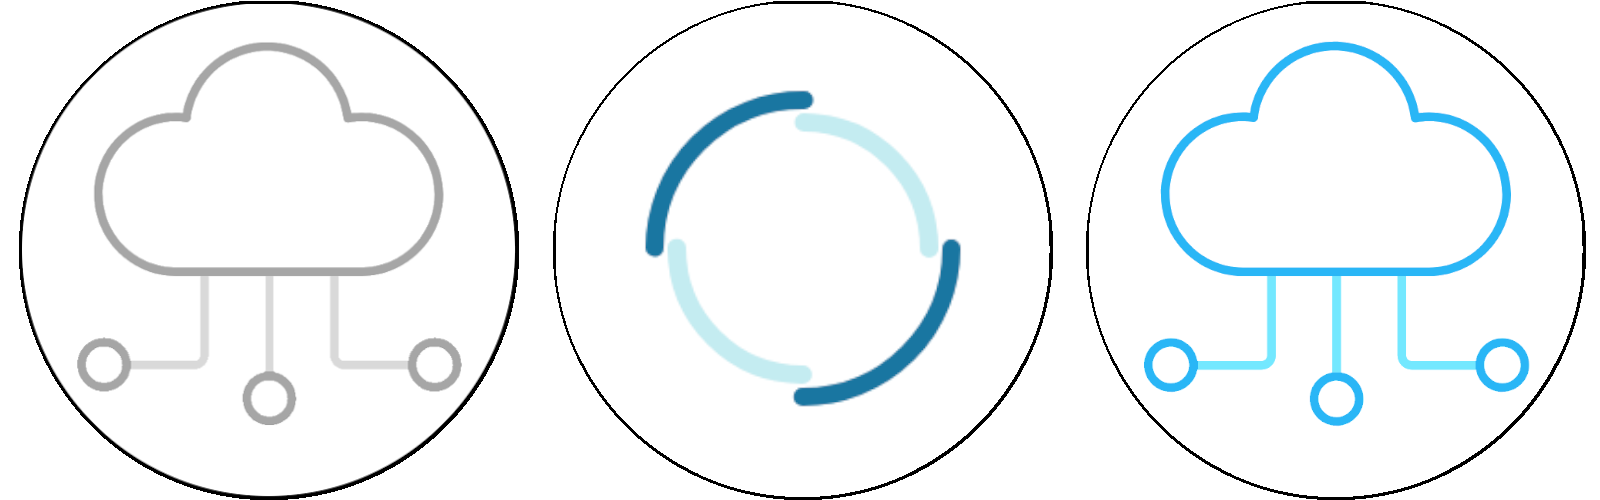
\includegraphics[width=0.6\textwidth]{Connection-Symbols.png}
    \caption{Symbole der Verbindungszustände} 
\end{figure}
\noindent
Neben dem Verbindungszustand wird auch die aktuelle Internetgeschwindigkeit in Form von verschiedenen Symbolen, welche in Figma erstellt wurden, angezeigt.
\\ \ \\
In Abbildung 7.2 sind die Symbole der Internetgeschwindigkeit von keiner Verbindung bis hin zur einer schnellen Internetgeschwindigkeit dargestellt.
\\
\begin{figure}[H]
    \centering
    
\includegraphics[width=0.4\textwidth]{Speed-Symbols.png}
    \caption{Verschiedene Symbole der Internetgeschwindigkeit} 
\end{figure}

\pagebreak

\subsubsection{Design des Zustandes Not Connected}

Der Startzustand, welcher direkt nach dem Öffnen der Desktop-Anwendung angezeigt wird ist der Not Connected-Zustand. In diesem Zustand wird der Hintergrund mit der Farbe Rot angezeigt. Das Textfeld in der Mitte der Anwendung zeigt hierbei immer den aktuellen Zustand, in diesem Fall Not Connected, an. Weiters lassen das ausgegraute Verbindungssymbol in der Mitte, sowie das durchgestrichene Geschwindigkeitssymbol am rechten oberen Rand darauf schließen, dass man aktuell mit keinem Server verbunden ist.
Der im unteren Teil der Desktop-Anwendung befindliche Connect-Button zeigt dem Benutzer mit dem Text Select Server, dass ein Server zum Verbinden ausgewählt werden muss.
\\ \ \\
Mit einem Klick auf den Pfeil, welcher sich auf der rechten Seite des Connect-Buttons befindet, öffnet sich eine DropUp-Liste mit allen zuvor im Menü hinzugefügten Servern. Nachdem man den gewünschten Server ausgewählt hat ändert sich die Farbe des Button auf intensiveres Grün und der Text auf Connect to \textit{Servername}. Hiermit wird dem Benutzer signalisiert, dass nun durch einen Mausklick auf die Mitte des Buttons der Verbindungsaufbau mit dem gewählten Server gestartet werden kann.
\\
\begin{figure}[H]
    \centering
    \setlength{\fboxsep}{1pt}
	\setlength{\fboxrule}{1pt}
	\fbox{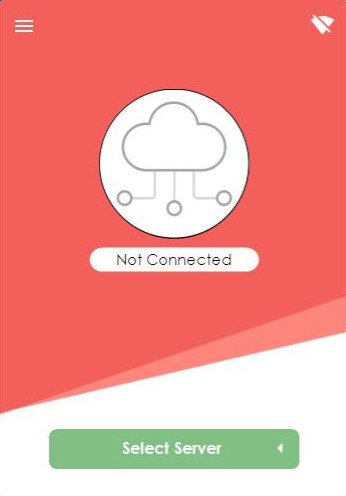
\includegraphics[width=0.4\textwidth]{NotConnected.jpg}}
    \caption{Design der Desktop-Anwendung im Zustand Not Connected} 
\end{figure}

\pagebreak

\subsubsection{Design des Zustandes Connecting}

Startet der Benutzer den Verbindungsaufbau, wechselt die Desktop-Anwendung in den Zustand Connecting. Hier wird der Hintergrund in der Farbe Blau angezeigt. Weiters ändert sich die Farbe des Buttons zu Grau und der Pfeil, welcher die Serverauswahl öffnet, verschwindet. Somit kann in der Zeit des Verbindens kein neuer Server ausgewählt werden. Auch kann nicht auf das Menü-Icon, welches die Einstellungen öffnet, gedrückt werden. Das Textfeld in der Mitte der Anwendung zeigt nun Connecting an und die animierte Ladeanimation deutet darauf hin, dass sich der Treiber mit dem ausgewählten Server verbindet.
\\
\begin{figure}[H]
    \centering
    \setlength{\fboxsep}{1pt}
	\setlength{\fboxrule}{1pt}
	\fbox{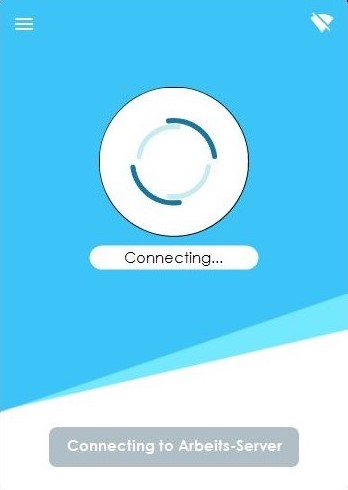
\includegraphics[width=0.4\textwidth]{Connecting.jpg}}
    \caption{Design der Desktop-Anwendung im Zustand Connecting} 
\end{figure}

\subsubsection{Design des Zustandes Connected}

Nach einem erfolgreichen Verbindungsaufbau wechselt die Desktop-Anwendung in den dritten Zustand Connected. In diesem Zustand wird der Hintergrund in der Farbe Grün angezeigt. Das Textfeld in der Mitte der Anwendung sagt nun “Connected to Servername”. Weiters lässt das darüberliegende Verbindungssymbol darauf schließen, dass man mit dem Server verbunden ist. Der Connect-Button hat sich auf die Farbe Rot und der Text auf Disconnect geändert. Das im rechten oberen Eck der Desktop-Anwendung befindliche Internetgeschwindigkeitssymbol hat neben der visuellen Darstellung nun auch eine weitere Funktion. Wenn man mit der Maus über das Symbol fährt erscheint links daneben eine Anzeige, welches dem Benutzer Auskunft über die aktuelle Internetgeschwindigkeit im Format Megabit pro Sekunde sowie den aktuellen Ping im Format Millisekunden gibt.
\\
\begin{figure}[H]
    \centering
    \setlength{\fboxsep}{1pt}
	\setlength{\fboxrule}{1pt}
	\fbox{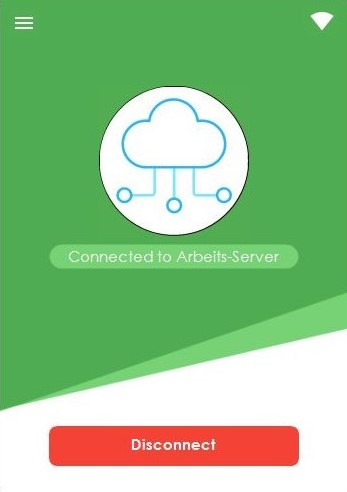
\includegraphics[width=0.4\textwidth]{Connected.jpg}}
    \caption{Design der Desktop-Anwendung im Zustand Conneted} 
\end{figure}

\subsubsection{Design des Fensters}

Viele Komponenten der Desktop-Anwendung wie Buttons und Textfelder haben ein modernes Design mit abgerundeten Ecken. Um eine einheitliche Designsprache zu gewährleisten soll auch das Fenster runde Ecken bekommen. Hierfür muss die Dynamic Link Library Gdi32\footnote[1]{\cite[Vgl.][]{GDI}} von Windows importiert werden. Diese beinhaltet die Methode \mbox{CreateRoundRectRgn()}, mit welchem ein neues Fenster mit angegebener Ellipsengröße für die Ecken erstellt werden kann.

\begin{program}[H]
\begin{CSharpCode}
Region = Region.FromHrgn(CreateRoundRectRgn(0, 0, Width, Height, 10, 10));
\end{CSharpCode}
\caption{Erstellen eines neuen Fensters mit abgerundeten Ecken}
\end{program}

\subsection{Design und Funktionalität des Connect-Buttons}

Der Connect-Button ist einer der wichtigsten Elemente der Desktop-Anwendung. Mithilfe diesem ist es möglich einen Server auszuwählen und sich mit diesem zu verbinden. Nach einem erfolgreichen Verbindungsaufbau kann man mit dem selben Button die Verbindung zum Server wieder trennen. Zusätzlich zur beschriebenen Funktionalität soll das Bedienelement über ein modernes Design mit abgerundeten Ecken verfügen.
\\ \ \\
Möchte man nun einen Button mit genau diesen Anforderungen in die Realität umsetzen, stößt man in WinForms mit den Standard-Windows-Bedienelementen auf drei wesentliche Probleme.
\\
\begin{enumerate}
 \item Der Standard-Button von WinForms ist viereckig und es gibt keine Möglichkeit dies zu ändern.
 \item Der Button soll über ein DropUp-Menü verfügen, welches eine Liste von Servern beinhaltet. Weiters soll man durch einen Mausklick auf diesen einen der Server auswählen können um sich damit zu verbinden. WinForms bietet zwar für solche Fälle eine sogenannte ComboBox an, doch diese hat erstens nur ein DropDown-Menü und zweitens stößt man bei der Benutzung dieser Komponente auf ein weiteres, nun folgendes Problem.
 \item Der Button soll zweigeteilt sein. Das bedeutet dass durch das Klicken auf das Bedienelement einerseits das Verbinden mit einem Server, andererseit aber auch das Öffnen des DropUp-Menüs möglich sein muss. Somit muss je nach Position des Mauszeigers beim Klick auf den Button eine andere Funktionalität verfügbar sein was mit dem Standard-Button ebenfalls nicht umsetzbar ist.
\end{enumerate}
\ \\
Die von uns verwendete Dynamic Link Library MetroSuite bietet zwar einen eigenen sogenannten MetroButton bei welchem man per Einstellung die Kanten abrunden kann, doch die 2 anderen Probleme können auch mit der Benutzung der DLL nicht gelöst werden. Daher können wir die Standard-Windows-Bedienelemente nicht benutzen und müssen einen eigenen Button programmieren.
\\ \ \\
In Abbildung 7.6 sind das gewünschte Design und die Funktionalität des Connect-Buttons dargestellt.
\begin{figure}[H]
    \centering
    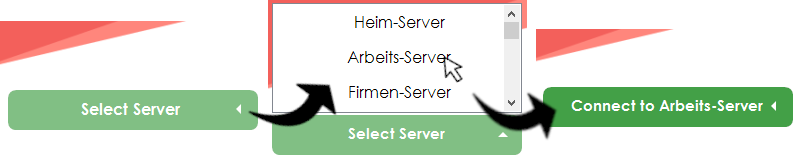
\includegraphics[width=1\textwidth]{connectButton.png}
    \caption{Design und Funktionalität des Connect-Buttons} 
\end{figure}

\subsubsection{Inhalt der Klasse Connect-Button}

Um einen eigenen Button mit unseren Wünschen zu kreieren, haben wir eine eigene Klasse namens ConnectButton, welche von der Standard-Button-Klasse abgeleitet ist, geschrieben. Die Button-Klasse ist Teil des System.Windows.Form-Namespaces, welcher alle User-Interface-Komponenten von Windows beinhaltet. Somit benutzen wir die schon vorhandenen Funktionalitäten eines Windows-Buttons und ergänzen diese mit eigenen zusätzlichen Funktionen und einem neuen Design.
\\ \ \\
Zum Designen des neuen Buttons benutzen wir die Klasse GraphicsPath, welche Teil vom System.Drawing.Drawing2D-Namespace ist. Mithilfe dieser Klasse ist es möglich Formen und Figuren mit der integrierten Grafik-Engine zu erstellen. Hierfür stellt die Klasse eine Reihe an Methoden zur Verfügung, mit welchen man neue Formen zu seiner Figur hinzufügen kann. In unseren Fall wurde die beiden Methoden AddLine() und AddArc() verwendet. Mithilfe dieser konnte die Form eines Buttons mit vier Linien und vier runden Ecken nachgebildet werden.

\begin{program}[H]
\begin{CSharpCode}
GraphicsPath graphPath = new GraphicsPath();
graphPath.AddLine(x1, y1, x2, y2);
\end{CSharpCode}
\caption{Hinzufügen einer Linie zu einer Figur}
\end{program}
\noindent 
Damit die erstellte Figure auch gezeichnet wird, muss noch die OnPaint-Methode der abgeleiteten Klasse Button überschrieben werden. In dieser Methode würde normalerweise der Standard-Windows-Button gezeichnet werden. Da hier aber jetzt unsere eigene Figure gezeichnet werden soll löschen wir das bestehende Design und zeichnen mit der Methode FillPath() die neue Figur.

\begin{program}[H]
\begin{CSharpCode}
protected override void OnPaint(PaintEventArgs paintEvent)
{
    paintEvent.Graphics.FillPath(brush, graphPath);
}
\end{CSharpCode}
\caption{Zeichnen einer Figur}
\end{program}
\noindent 
Wenn man nun den Connect-Button erstellt wird man bemerken, dass dieser vor allem in den Ecken nicht schön rund sondern eher verpixelt von der Grafik-Engine gezeichnet wurde. Um diesem Problem entgegenzuwirken müssen in der OnPaint()-Methode noch einige Einstellungen über die Renderqualität getätigt werden.

\begin{program}[H]
\begin{CSharpCode}
paintEvent.Graphics.InterpolationMode = InterpolationMode.HighQualityBilinear;
paintEvent.Graphics.CompositingQuality = CompositingQuality.HighQuality;
paintEvent.Graphics.PixelOffsetMode = PixelOffsetMode.HighQuality;
paintEvent.Graphics.SmoothingMode = SmoothingMode.AntiAlias;
\end{CSharpCode}
\caption{Beispiel-Code zum Verbessern der Renderqualität}
\end{program}
\noindent 
Mithilfe dieser vier Methoden werden alle wichtigen, für die Zeichen- und Renderqualität verantwortlichen Parameter auf die maximale Qualität gestellt um die bestmögliche Grafik zu erzielen. 
\\ \ \\
Neben einem Text soll auf der rechten Seite des Connect-Buttons auch ein Pfeil angezeigt werden, welcher dem Benutzer zeigt, dass man mit einem Mausklick auf diesen die Drop-Up-Liste öffnen beziehungsweise schließen kann. Dieser Pfeil soll je nachdem ob die Liste gerade geöffnet oder geschlossen ist, nach oben oder nach links zeigen. Hierfür wurden zwei verschiedene Pfeile für die beiden Richtungen in Figma kreiert. Die beiden Grafiken werden mithilfe der Klasse Icon eingelesen und können dann mit der Methode DrawIcon() an einer bestimmten Stelle im Button gezeichnet werden. Wichtig hierbei ist, dass die eingebundenen Icons vom Typ .ico sein müssen! 

\begin{program}[H]
\begin{CSharpCode}
Icon arrow = new Icon("arrow.ico");
paintEvent.Graphics.DrawIcon(arrow , x, y);
\end{CSharpCode}
\caption{Zeichnen eines Icons}
\end{program}
\noindent 
Da der Connect-Button durch das Klicken auf zwei verschiedene Stellen zwei verschiedene Funktionalitäten haben soll muss hier mit der Position des Mauszeigers beim Klick gearbeitet werden. Zuerst wird ein MouseUp-Event definiert, welches beim wieder Loslassen nach dem Drücken der linken Maustaste aktiviert wird. Nun kann mit MousePosition.X die X-Koordinate der aktuellen Position des Mauszeigers abgerufen werden. Mithilfe dieser Koordinate kann man überprüfen ob der Benutzer die Drop-Up-List aufrufen oder den Verbindungsaufbau starten möchte. Falls noch kein Server ausgewählt worden ist, ist der Mausklick zum Verbinden wirkungslos.

\subsubsection{Design und Funktionalität der Drop-Up-Liste}

Die Drop-Up-Liste soll die Möglichkeit bieten einen Server auszuwählen, um sich mit diesem zu verbinden. Hierfür verwenden wir die ListBox von WinForms. Diese Komponente ermöglicht standardmäßig das Hinzufügen von Einträgen, das Auswählen dieser, sowie das Nutzen einer Scrollbar. Zusätzlich dazu wurde auch dieses UI-Element an unserer Wünsche angepasst und um einige Funktionalitäten erweitert. Das Ziel ist, genauso wie beim Connect-Button, das Design zu verbessern. Die Änderungen umfassen das Anpassen der Schriftart/-größe und der Position, sowie das Verhalten beim Auswählen eines Servers durch einen Mausklick auf diesen.
\\ \ \\
Um die gewünschten Änderungen umzusetzen muss nicht wie beim Connect-Button eine eigene Klasse erstellt und die OnPaint()-Methode überschrieben werden. Hierfür gibt es das ListBox-Event DrawItem. Mithilfe von Events und Delegates ist es also möglich eine eigene Methode zu schreiben, mit welcher man die Elemente der ListBox selbst zeichnen kann. Wichtig zu erwähnen ist, dass wenn man diese Methode verwenden möchte, vorher noch die Option DrawMode der ListBox auf OwnerDrawFixed gestellt werden muss!
\\ \ \\
Nun haben wir die Möglichkeit, das Verhalten beim Auswählen eines Listenelementes zu definieren. Hierfür wird mit einem If-Anweisung überprüft ob das Listenelement ausgewählt wurde. Falls das der Fall ist, wird die Schriftart auf Fett geändert und die Schriftfarbe auf Grün.

\begin{program}[H]
\begin{CSharpCode}
if (drawEvent.State == DrawItemState.Selected)
{
    drawEvent = new DrawItemEventArgs(/*Parameter*/);
}
\end{CSharpCode}
\caption{Ändern der Eigenschaften eines ausgewählten Listenelements}
\end{program}
\noindent
Nach dem Definieren aller weiteren Parameter, wie Standard-Schriftart, -farbe und -größe muss das Listenelement noch gezeichnet werden. Hierfür kommt die Methode DrawString() zum Einsatz. Da hier auch Informationen über die Position angegeben werden müssen, kann so auch gleich definiert werden, dass das Element mittig in der ListBox zentriert gezeichnet werden soll.

\begin{program}[H]
\begin{CSharpCode}
drawEvent.Graphics.DrawString(text, font, brush, x, y);
\end{CSharpCode}
\caption{Zeichnen eines Listenelementes}
\end{program}
\noindent
Zum Einstellen des Abstandes zwischen den Listenelementen gibt es die ListBox-Eigenschaft ItemHeight. Mithilfe dieser kann der gewünschte Wert definiert werden. Hierfür muss aber die Option DrawMode der ListBox auf OwnerDrawVariable gestellt werden.

\subsection{Design und Funktionalität des Menüs}
Mit einem Mausklick auf das Icon in der linken oberen Ecke der Desktop-Anwendung gelangt man in das Menü. Hier können wichtige Einstellungen getätigt werden. Das Menü ist in die drei Menüpunkte Mode, Server und Network Devices unterteilt. Jeder der Menüpunkte wird durch ein eigenes, zur Einstellungsmöglichkeit passendes, Icon repräsentiert. Diese wurden in Figma erstellt. Mit einem Klick auf den jeweiligen Unterpunkt kommt man zu deren spezifischen Einstellungen. Um das Menü wieder zu verlassen, muss man auf den Schließen-Button, welcher sich oben links befindet klicken.
\\
\begin{figure}[H]
    \centering
    \setlength{\fboxsep}{1pt}
	\setlength{\fboxrule}{1pt}
	\fbox{\includegraphics[width=0.4\textwidth]{Menü.jpg}}
    \caption{Design des Menüs mit den drei Menüpunkten} 
\end{figure}

\pagebreak
\subsubsection{Design des Menüpunktes Mode}

Bei den Modus-Einstellungen, kann man definieren in welchem Modus der Treiber laufen soll. Man soll zwischen dem Perfomance-basierenden und Kostenbasierenden Modus auswählen können. Da wir uns im Rahmen der Diplomarbeit ausschließlich auf den ersten der beiden Modis konzentrieren dient der Menüpunkt Mode aktuell nur als Beschreibung des Kosten-basierenden Modus. Der ausgegraute Button mit dem Text “Selected” unterhalb der Kurzbeschreibung zeigt dem Benutzer, dass akutell dieser Modus ausgewählt ist. Mit einem Klick Mausklick auf den Pfeil links oben kommt man wieder in die Einstellungsübersicht zurück.
\\
\begin{figure}[H]
    \centering
    \setlength{\fboxsep}{1pt}
	\setlength{\fboxrule}{1pt}
	\fbox{\includegraphics[width=0.4\textwidth]{MenüMode.jpg}}
    \caption{Design des Menüpunktes Mode} 
\end{figure}

\subsubsection{Design des Menüpunktes Server}

Bei den Server-Einstellungen hat der Benutzer die Möglichkeit, Server zu verwalten.
Im oberen Bereich mit der Aufschrift “Add Server” kann man einen neuen Server hinzuzufügen. Hier muss der Name, welcher frei wählbar ist, die IP-Adresse und der Post des Servers eingetragen werden. Mit einem Klick auf “Add” wird der Server in die darunterliegende Liste hinzugefügt. Im unteren Bereich namens “Server List” werden alle gespeicherten Server angezeigt. Mit einem Mausklick auf einen Server wird die Schriftart Fett und die Schriftfarbe Blau angezeigt. Somit wurde der Server als Default-Server festgelegt. Mit dem Löschen-Button, welcher sich unterhalb der Liste befindet, kann ein ausgewählter Server wieder von der Liste entfernt werden.
\\
\begin{figure}[H]
    \centering
    \setlength{\fboxsep}{1pt}
	\setlength{\fboxrule}{1pt}
	\fbox{\includegraphics[width=0.4\textwidth]{MenüServer.jpg}}
    \caption{Design des Menüpunktes Server} 
\end{figure}
\noindent
WinForms bietet keine Möglichkeit, das Verhalten bei der Auswahl eines Listenelementes zu ändern. Daher kamen genauso wie bei der Drop-Up-Liste des ConnectButtons Event, Delegates und die Methode DrawItem() zum Einsatz um die Listenelement manuell zu zeichnen. Nur so konnte das Ändern der Schrifteigenschaften möglich gemacht werden.

\subsubsection{Speichern der Serverliste}
Da zur Serverliste hinzugefügte Server auch nach dem Schließen und einem erneuten Öffnen der Desktop-Anwendung noch zur Verfügung stehen sollen, müssen wichtige Einstellungen wie die Serverliste gespeichert werden. Hierfür benutzen wird den System.Text.Json-Namespace welcher es ermöglicht, Objekte ins JSON-Format zu serialisieren und vom JSON-Format wieder in Objekte zu deserialisieren.
\\ \ \\
Zur Speicherung relevante ist eine Liste mit allen Servern, welche wiederum aus den drei Attributen Name, IP-Adresse und Port bestehen. Um diese Daten einfach zu speichern und später wieder auslesen zu können haben wir eine Klasse namens ServerObject erstellt, welche die drei Attribute beinhaltet. Eine zweite Klasse ServerSettings speichert diese Server-Objekte in einer Liste.

\begin{program}[H]
\begin{CSharpCode}
public class ServerObject
{
    public string name { get; set; }
    public string ip { get; set; }
    public int port { get; set; }
}
\end{CSharpCode}
\caption{Aufbau der Klasse ServerObject}
\end{program}
\noindent
Wird nun ein neuer Server in der Desktop-Anwendung hinzugefügt, wird ein neues Server-Objekt erstellt und in die Serverliste hinzugefügt. Sollte ein bestehender Server gelöscht werden, wird das Server-Objekt wieder aus der Liste entfernt.
\\ \ \\
Schließt der Benutzer nun die Desktop-Anwendung werden mögliche Änderungen in der Serverliste gespeichert werden. Hierfür kommt der im System.Text.Json-Namespace enthaltene JsonSerializer zum Einsatz. Dieser serialisiert ein ServerSettings-Objekt, welches die Liste mit allen Servern-Objekten beinhaltet, zu einem JSON-Text. Dieser wird dann in eine Datei names serverSettings.json im selben Verzeichnis wo auch die .exe-Datei liegt gespeichert.

\begin{program}[H]
\begin{CSharpCode}
public class ServerObject
string settings = JsonSerializer.Serialize(serverSettings);
\end{CSharpCode}
\caption{Serialisieren des serverSettings-Objektes}
\end{program}
\noindent
Startet der Benutzer die Desktop-Anwendung, werden alle gespeicherten Einstellungen wieder geladen. Hierfür wird der gespeicherte JSON-Text aus der Datei ausgelesen und mit dem JsonSerializer deserialisiert.

\begin{program}[H]
\begin{CSharpCode}
serverSettings = JsonSerializer.Deserialize<ServerSettings>(settings);
\end{CSharpCode}
\caption{Deserialisieren des eingelesenen JSON-Textes}
\end{program}
\noindent
Nachdem das einlesen erfolgreich abgeschlossen wurde, werden die Serverliste im Menü sowie die Drop-Up-List vom Connect-Button mit den gespeicherten Einstellungen befüllt.

\subsubsection{Design des Menüpunktes Network Devices}

Bei den Netzwerkadapter-Einstellungen kann der Benutzer die Netzwerkadapter verwalten. Hierfür werden im Bereich mit der Aufschrift \grqq Network Devices List\grqq{} alle verfügbaren Netzwerkadapter aufgelistet. Durch einen Mausklick auf einen Listeneintrag wird die Schriftart Fett und die Schriftfarbe Blau. Somit wurde der Netzwerkadapter ausgewählt und wird nun vom Treiber verwendet. Mit einem erneuten Klick kann dieser auch wieder abgewählt werden. Für die Erweiterung des Kosten-basierenden Modus, würde noch die Angabe der Kosten pro Megabyte hinzukommen.
\\
\begin{figure}[H]
    \centering
    \setlength{\fboxsep}{1pt}
	\setlength{\fboxrule}{1pt}
	\fbox{\includegraphics[width=0.4\textwidth]{MenüNetworkDevices.jpg}}
    \caption{Design des Menüpunktes Network Devices} 
\end{figure}

\subsubsection{Einlesen der Netzwerkadapter}

Um die Netzwerkadapter auswählen zu können, müssen diese beim Start der Desktop-Anwendung eingelesen werden. Hierfür muss die Klasse Win32\_NetworkAdapterConfiguration instanziiert werden. Diese beinhaltet alle Attribute und Methoden der Netzwerkadapter. Das Attribut Description liefert uns den Namen des Netzwerkadapters, welchen wir in die Network-Devices-Liste speichern können. Mithilfe der Variable ipEnabled werden nur aktivierten Netzwerkadapter angezeigt.

\begin{program}[H]
\begin{CSharpCode}
if ((bool)managementObject["ipEnabled"])
{
    netDevices.Add(managementObject["Description"].ToString());
}
\end{CSharpCode}
\caption{Einlesen der Namen der aktiven Netzwerkadapter}
\end{program}
\noindent
Da die Namen der Netzwerkadapter oft zu breit für die Darstellung in der ListBox sind, muss gegebenenfalls eine horizontale Scrollbar angezeigt werden. Hierfür wird nach dem Einfügen der Adapter mithilfe der MeasureString()-Methode die Länge der Namen ermittelt.

%Setzen der Schriftgröße für die Code-Beispiele von Martin
\lstset{basicstyle=\footnotesize}

\pagebreak

\section{Desktop-Anwendung in der Notification Area}
Wir haben unsere Windows Desktop-Anwendung zum Steuern des Multi-Wan Bonding fähigen Treibers als Notification Area Programm entwickelt. Dabei war es uns sehr wichtig, dass der Benutzer einmal auf das Symbol klicken kann, damit wird ihm die wie im Kapitel 7.1 beschriebene Benutzeroberfläche angezeigt. Wenn er jetzt nochmals darauf oder woanders hin drückt, soll die Benutzeroberfläche verborgen werden
\\\\
Um eine Notification Area Anwendung zu implementieren, haben wir eine C\# Klasse entwickelt, diese Klasse ist von \textbf{ApplicationContext} abgeleitet. In dieser Klasse wird ein \textbf{NotifyIcon} angelegt. Dieses \textbf{NotifyIcon} benötigt ein Symbol, mit diesem wird dann die Anwendung in der Notfication Area abgelegt, einen Text der erscheint, sobald sich die Maus über dem Symbol befindet, in unserem Fall "NetShare". Weiters hat das Symbol einen Button zum Schließen der Anwendung, sobald das Symbol mit der rechten Maustaste angeklickt wurde. Wenn dieser Knopf gedrückt wird beendet sich die Windows Desktop-Anwendung und auch der Multi-Wan Bonding fähige Treiber.
\begin{figure}[H]
    \centering
    
\includegraphics[width=5cm, height=5cm, keepaspectratio]{NAIcon.png}
    \caption[NotificationArea]{Netshare Symbol in der Notification Area} 
\end{figure}
\noindent

\newpage
\subsection{Relative Positionierung der grafischen Oberfläche}
Die Grafische Oberfläche der Windows Desktop-Anwendung soll sich immer an der richtigen Stelle relativ zur Taskleiste positionieren. Mithilfe von \textbf{Screen.PrimaryScreen.Bounds} und \textbf{Screen.PrimaryScreen.WorkingArea} finden wir heraus wo sich die Taskleiste befindet. Mit diesem Wissen setzen wir dann die relative Positionierung der grafischen Oberfläche. \textbf{Screen.PrimaryScreen.Bounds} gibt einem die gesamte Größe des Bildschirms an, \textbf{Screen.PrimaryScreen.WorkingArea} gibt einem die Größe an in der z.B. auch Webbrowser geöffnet sind, also ohne der  Taskleiste. Im Codebeispiel sieht man wie dies funktioniert, wenn sich die Taskleiste am unteren Rand befindet.
\begin{program}[H]
\caption{Taskleiste unten}
\begin{CSharpCode}
if((Screen.PrimaryScreen.Bounds.Height - Screen.PrimaryScreen.WorkingArea.Height)>0)
{
    this.Location = new Point(Screen.PrimaryScreen.WorkingArea.X + 
      Screen.PrimaryScreen.WorkingArea.Width - Width - 10, 
      Screen.PrimaryScreen.WorkingArea.Y + Screen.PrimaryScreen.WorkingArea.Height 
      - Height);
}
\end{CSharpCode}
\end{program}
\noindent

\section{Kommunikation zwischen dem Multi-Wan Bonding fähigen Treiber und der Windows Desktop-Anwendung}
Die Windows-Desktop Anwendung muss für das Steuern des Multi-Wan Bonding fähigen Treibers mit diesem Kommunizieren. Wir haben uns als Interprozesskommunikationsart für Sockets entschieden, da wir dies für am einfachsten angesehen haben, weil man sich nicht um die Synchronisation kümmern muss. Der Multi-Wan Bonding fähige Treiber erstellt einen Server der auf "localhost" \ auf dem Port 5260 lauscht und wartet bis sich ein Client mit ihm verbindet. Die Windows Desktop-Anwendung erstellt für jeden Steuerungsbefehl an den Multi-Wan Bonding fähigen Treiber einen Client, der sich zum Server verbindet und dann ein JSON Objekt mit dem jeweiligen Befehl zum Server sendet. Sobald die Windows Desktop-Anwendung die erwartete Antwort bekommen hat, wird die Verbindung zum Multi-Wan Bonding fähigen Treiber geschlossen.

\newpage
\subsection{JSON Object}
\subsubsection{Anfrage (Request)}
Wenn die Windows Desktop-Anwendung eine Anfrage an den Multi-Wan Bonding fähigen Treiber sendet, hat das JSON Objekt folgende Struktur.
\begin{program}[H]
\caption{JSON Anfrage}
\begin{GenericCode}
    {
        "type" :  "",
        "on" :  "",
        "data" : {} 
    }
\end{GenericCode}
\end{program}
\noindent
Bei dem Schlüssel \textbf{type} wird vom Multi-Wan Bonding fähigen Treiber \textbf{Get} oder \textbf{Put} erwartet. Mit \textbf{Get} kann die Windows-Desktop Anwendung die derzeitige Konfiguration oder die Download und Upload Geschwindigkeiten des Multi-Wan Bonding fähigen Treibers anfordern. Mithilfe von \textbf{Put} werden Einstellungen hinzugefügt oder geändert. 
\\\\
Bei dem Schlüssel \textbf{on} gibt es die Werte \textbf{driver.state}, \textbf{deamon.state}, \textbf{connection.state}, \textbf{config} und \textbf{statistics}. Mit \textbf{driver.state} verbindet sich der Multi-Wan Bonding fähige Treiber mit dem Multi-Wan Bonding fähigen Server oder bricht die Verbindung ab. Mithilfe von \textbf{deamon.state} kann man den Multi-Wan Bonding fähigen Treiber beenden. Mit \textbf{connection.state} kann man die Verbindung zwischen dem Server und dem Client von der Server Seite aus beenden und mit \textbf{config} kann man die derzeitigen Konfigurationen anpassen oder anfordern. Mit dem Wert \textbf{statistics} erhält man die Download und Upload Geschwindingkeiten.
\\\\
Bei dem Schlüssel \textbf{data} wird der Wert \textbf{state} erwartet, falls bei dem Schlüssel on der Wert \textbf{driver.state}, \textbf{deamon.state} oder \textbf{connection.state} ist. Wenn der vorherige Schlüssel \textbf{config} ist, wird bei \textbf{data} entweder \textbf{logLevel}, \textbf{serverIp}, \textbf{adapterIp}, \textbf{adapterSubnetBits}, \textbf{names} oder nichts, falls man die gesamte Konfiguration erhalten will, dies ist aber nur möglich, wenn bei dem Schlüssel \textbf{type} der Wert \textbf{Get} ist. Wenn beim Schlüssel \textbf{on} \textbf{statistics} steht, ist wird in \textbf{data} ebenfalls nichts erwartet. 


\subsubsection{Antwort (Response)}
Wenn der Multi-Wan Bonding Server eine Antwort an die Windows-Desktop Anwendung sendet, ist das JSON Objekt folgendermaßen aufgebaut.
\begin{program}[H]
\caption{JSON Antwort}
\begin{GenericCode}
    {
        "type" :  "",
        "data" : {}
    }
\end{GenericCode}
\end{program}
\newpage
\noindent
Bei dem Schlüssel \textbf{type} gibt es zwei mögliche Werte entweder \textbf{Response} oder \textbf{Update}. Mit \textbf{Response} wird mitgeteilt das eine Anfrage fertig abgearbeitet ist. Mithilfe von \textbf{Update} wird ausgedrückt, dass der Multi-Wan Bonding fähige Treiber etwas geändert hat.
\\\\
Beim Schlüssel \textbf{data} steht, falls ein Fehler aufgetreten ist \textbf{error}, ansonsten \textbf{state}, der angeforderte Konfigurationswert, alle konfigurierten Werte mit dem jeweiligen Werten drinnen oder \textbf{down} mit einem Wert und \textbf{up} mit einem Wert.  


\subsection{Verbinden des Multi-Wan Bonding fähigen Treibers mit einem Multi-Wan Bonding fähigen Server}
Um mithilfe des Multi-Wan Bonding fähigen Treibers die Verbindung zum Multi-Wan Bonding fähigen Server herzustellen, wird eine Anfrage von der Windows-Desktop Anwendung gesendet. Diese Anfrage ist folgendermaßen aufgebaut:
\begin{program}[H]
\caption{JSON Anfrage verbinden}
\begin{GenericCode}
    {
        "type" :  "Put",
        "on" :  "driver.state",
        "data" : {"state" : "running"} 
    }    
\end{GenericCode}
\end{program}
\noindent
Daraufhin checkt der Multi-Wan Bonding fähige Treiber ob dieser schon mit dem Multi-Wan Bonding fähigen Server verbunden ist, falls dies der Fall ist, wird diese Antwort gesendet:
\begin{program}[H]
\caption{JSON Antwort verbinden running}
\begin{GenericCode}
    {
        "type" :  "Response",
        "data" : {"state" : "running"} 
    }    
\end{GenericCode}
\end{program}
\noindent
Falls der Multi-Wan Bonding fähige Treiber sich gerade mit dem Multi-Wan Bonding fähigen Server verbindet oder noch keine Verbindung aufgebaut ist, wird beim Schlüssel \textbf{state} der Wert \textbf{startup} eingetragen und als Antwort gesendet. Nachdem die Verbindung erfolgreich aufgebaut wurde, wird das JSON Objekt von vorher gesendet. Wenn die Verbindung nicht aufgebaut werden kann, bekommt man folgende Antwort:
\begin{program}[H]
\caption{JSON Antwort verbinden crashed}
\begin{GenericCode}
    {
        "type" :  "Response",
        "data" : {"state" : "crashed"} 
    }    
\end{GenericCode}
\end{program}
\newpage
\noindent
Nachdem man diese Antwort bekommen hat, versucht die Windows Desktop-Anwendung es noch zweimal, indem sie wieder die Anfrage an den Multi-Wan Bonding fähigen Treiber sendet. Falls bei den zwei weiteren Anfragen auch nur der Wert \textbf{crashed} bei dem Schlüssel \textbf{state} zurückkommt, wird dem Benutzer eine Fehlermeldung angezeigt, die Ihn dazu auffordert den Multi-Wan Bonding fähigen Treiber neu zu starten.


\subsection{Verbindung zu einem Multi-Wan Server trennen}
Um die Verbindung zwischen dem Multi-Wan Bonding fähigen Treiber und dem Multi-Wan Bonding fähigen Server zu trennen, wird eine Anfrage von der Windows Desktop-Anwendung gesendet. Diese Anfrage ist folgendermaßen aufgebaut:
\begin{program}[H]
\caption{JSON Anfrage Verbindung trennen}
\begin{GenericCode}
    {
        "type" :  "Put",
        "on" :  "driver.state",
        "data" : {"state" : "stopped"} 
    }     
\end{GenericCode}
\end{program}
\noindent
Der Multi-Wan Bonding fähige Treiber sendet als Antwort seinen derzeitigen Status, diese Antwort wird so gesendet:
\begin{program}[H]
\caption{JSON Antwort Verbindung trennen}
\begin{GenericCode}
    {
        "type" :  "Response",
        "data" : {"state" : ""} 
    }    
\end{GenericCode}
\end{program}
\noindent
Wobei bei dem Schlüssel \textbf{state} entweder der Wert \textbf{startup}, \textbf{running} oder \textbf{stopped} steht. Falls der Multi-Wan Bonding fähige Treiber als Status nicht \textbf{stopped} hat, bricht der Multi-Wan Bonding fähige Treiber die Verbindung zum Multi-Wan Bonding fähigen Server ab und sendet die Antwort an die Windows Desktop-Anwendung die als \textbf{state} \textbf{stopped} hat.


\subsection{Multi-Wan Bonding fähigen Treiber beenden}
Um den Multi-Wan Bonding fähigen Treiber zu beenden, wird eine Anfrage von der Windows Desktop-Anwendung gesendet. Diese Anfrage ist folgendermaßen aufgebaut:
\begin{program}[H]
\caption{JSON Anfrage Treiber beenden}
\begin{GenericCode}
    {
        "type" :  "Put",
        "on" :  "deamon.state",
        "data" : {"state" : "stopped"} 
    }     
\end{GenericCode}
\end{program}
\newpage
\noindent
Der Multi-Wan Bonding fähige Treiber sendet im Sekundentakt eine Antwort in dieser steht, was der Multi-Wan Bonding fähige Treiber gerade macht. Die Antwort wird mit diesem Aufbau gesendet:
\begin{program}[H]
\caption{JSON Antwort Treiber beenden}
\begin{GenericCode}
    {
        "type" :  "Update",
        "data" : {"state" : ""} 
    }    
\end{GenericCode}
\end{program}
\noindent
Bei dem Schlüssel \textbf{state} steht als Wert entweder \textbf{worker.startup}, \textbf{worker.running} oder \textbf{worker.stopped}. Solange sich der Multi-Wan Bonding fähige Treiber im Status \textbf{startup} befindet, passiert nichts außer, dass die Antwort mit \textbf{worker.startup} sekündlich gesendet wird. Sobald der Status \textbf{running} ist, wird die Antwort mit \textbf{worker.running} gesendet und die Anwendung bekommt den Befehl sich zu schließen. Wenn dies geschehen ist, wird die Antwort mit \textbf{worker.stopped} gesendet. Zusätzlich dazu wird noch eine Antwort gesendet die als \textbf{type} \textbf{Response} hat und bei \textbf{state} den Wert \textbf{stopped} hat.


\subsection{Konfiguration des Multi-Wan Bonding fähigen Treibers ändern}
Um die Einstellungen von dem Multi-Wan Bonding fähigen Treiber zu ändern, wird von der Windows Desktop-Anwendung eine Anfrage gesendet, die folgendermaßen aufgebaut ist:
\begin{program}[H]
\caption{JSON Anfrage Konfiguration ändern}
\begin{GenericCode}
    {
        "type" :  "Put",
        "on" :  "config",
        "data" : {} 
    }     
\end{GenericCode}
\end{program}
\noindent
Bei dem Schlüssel \textbf{data} wird das zu konfigurierende Schlüssel Wert Paar eingetragen. Der Multi-Wan Bonding fähige Treiber sendet als Antwort folgendes JSON-Objekt:
\begin{program}[H]
\caption{JSON Antwort Konfiguration ändern}
\begin{GenericCode}
    {
        "type" :  "Response",
        "data" : {} 
    }    
\end{GenericCode}
\end{program}
\noindent
In \textbf{data} steht das geänderte Schlüssel Wert Paar. Die einzige Änderung die der Multi-Wan Bonding fähige Treiber sofort übernimmt, ist eine Änderung beim \textbf{logLevel}. Jede andere Änderung wird erst verwendet nachdem die Verbindung zum Multi-Wan Bonding fähigen Server getrennt wurde und sich neu mit diesem Verbunden wurde.


\subsection{Konfiguration des Multi-Wan Bonding fähigen Treibers anfordern}
\subsubsection{Gesamte Konfiguration}
Um die gesamte Konfiguration des Multi-Wan Bonding fähigen Treibers zu bekommen, wird von der Windows Desktop-Anwendung eine Anfrage gesendet, die folgendermaßen aufgebaut ist:
\begin{program}[H]
\caption{JSON Anfrage Gesamte Konfiguration anfordern}
\begin{GenericCode}
    {
        "type" :  "Get",
        "on" :  "config",
        "data" : {} 
    }     
\end{GenericCode}
\end{program}
\noindent
Wenn diese Anfrage gesendet wird, antwortet der Multi-Wan Bonding fähige Treiber folgendermaßen:
\begin{program}[H]
\caption{JSON Antwort Gesamte Konfiguration anfordern}
\begin{GenericCode}
    {
        "type" :  "Response",
        "data" : {
                    "logLevel" : "",
                    "serverIp" : "",
                    "serverPort" : "",
                    "adapterIp" : "",
                    "adapterSubnetBits" : "",
                    "names" : []
        } 
    }    
\end{GenericCode}
\end{program}
\noindent
Bei jedem Schlüssel Wert Paar in \textbf{data} wird noch der eingestellte Wert eingetragen.


\subsubsection{Einzelne Einstellungen}
Um nur eine einzelne Konfiguration vom Multi-Wan Bonding fähigen Treiber zu bekommen, wird eine Anfrage von der Windows Desktop-Anwendung gesendet, die folgendermaßen aufgebaut ist:
\begin{program}[H]
\caption{JSON Anfrage einzelne Konfiguration anfordern}
\begin{GenericCode}
    {
        "type" :  "Get",
        "on" :  "config",
        "data" : {} 
    }     
\end{GenericCode}
\end{program}
\noindent
In dem Feld \textbf{data} steht ein Schlüssel Wert Paar als Schlüssel steht die gewünschte Option und als Wert eine Leere Zeichenkette. Der Multi-Wan Bonding fähige Treiber sendet eine Antwort die folgendermaßen Aufgebaut ist: 
\begin{program}[H]
\caption{JSON Antwort einzelne Konfiguration anfordern}
\begin{GenericCode}
    {
        "type" :  "Response",
        "data" : {} 
    }    
\end{GenericCode}
\end{program}
\noindent
In \textbf{data} steht das angeforderte Schlüssel Wert Paar.

\subsection{Upload und Download Geschwindigkeit anfordern}
Um in der Windows Desktop-Anwendung den Upload und den Download Speed anzeigen zu können, wird eine Anfrage an den Multi-Wan Bonding fähigen Treiber gesendet, diese Anfrage ist folgendermaßen aufgebaut:
\begin{program}[H]
\caption{JSON Anfrage Upload Download}
\begin{GenericCode}
    {
        "type" :  "Get",
        "on" :  "statistics",
        "data" : {} 
    }     
\end{GenericCode}
\end{program}
\noindent
Der Multi-Wan Bonding fähige Treiber sendet daraufhin jede Sekunde eine Antwort mit der Upload und Download Geschwindigkeit, diese werden kontinuierlich berechnet. Die Antwort ist folgendermaßen aufgebaut:
\begin{program}[H]
\caption{JSON Antwort Upload Download}
\begin{GenericCode}
    {
        "type" :  "Response",
        "data" : {
                    "down" : "",
                    "up" : ""
        } 
    }    
\end{GenericCode}
\end{program}
\noindent
Die Anfrage an den Mult-Wan Bonding fähigen Treiber wird automatisch gesendet, sobald dieser mit einem Multi-Wan Bonding fähigen Server verbunden ist. 

%Setzen der Schriftgröße für die Code-Beispiele für Manuel
\lstset{basicstyle=\normalsize}

\pagebreak

\section{Windows-Service zur Crash-Recovery des Treibers}

Ein Windows-Service, zu deutsch Windows-Systemdienst, ist ein Programm welches als Dienst im Hintergrund einer Windows-Sitzung läuft\footnote[1]{\cite[Vgl.][]{WindowsService}}. Somit eignet sich ein Windows-Service perfekt für unseren Treiber, welcher immer im Hintergrund laufen, aber den Benutzer nicht stören soll. Weiters soll dieser, bei einem möglichen Absturz, automatisch vom Service neu gestartet werden.

\subsection{Starten des Treibers}

Beim Starten unseres Treibers in Form einer .exe-Datei muss bedacht werden, dass seit der Windows Version Vista ein Windows-Service nicht mehr mit dem Desktop interagieren kann. Das bedeutet, dass der Systemdienst keine Programme mit grafischer Oberfläche starten kann. Da unser Treiber keine grafischen Elemente besitzt kann dieser mit der Angabe von zusätzlichen Parametern gestartet werden.
Mit dem Kofigurieren der Parameter CreateNoWindow und UseShellExecute weiß der Windows-Service, dass keine grafische Oberfläche sowie Shell vom Treiber benutzt wird.

\begin{program}[H]
\begin{CSharpCode}
ProcessStartInfo info = new ProcessStartInfo("netshare.exe");

info.UseShellExecute = false;
info.CreateNoWindow = true;
info.ErrorDialog = false;
info.WindowStyle = ProcessWindowStyle.Hidden;

Process process = Process.Start(info);
\end{CSharpCode}
\caption{Starten des Treibers mit Windows-Service}
\end{program}

\subsection{Crash-Recovery}

Damit sichergestellt werden kann, dass der Treiber immer verfügbar ist, muss im Windows-Service eine Crash-Recovery eingebaut werden. Diese überprüft ob das Programm noch läuft und startet gegebenenfalls den Treiber neu. Das laufende Programm kann mithilfe von \mbox{Process.GetProcessesByName("netshare.exe")} gefunden und somit überprüft werden.
\chapter{Funktionstests für Multi-Wan Bonding}
\label{cha:Funktionstests für Multi-Wan Bonding}

\section{Testaufbau}
Beim Testen unseres Multi-Wan Bonding Prototyps haben wir die folgenden Tests durchgeführt. 

\subsection{Internetverbindung}
Um zu überprüfen, ob wir uns mithilfe unseres Prototyps eine Verbindung mit dem Internet aufbauen zu können, haben wir nur eine Internetanbindung verwendet und versucht google aufzurufen. Als dieses funktioniert hat, haben wir das selbe mit zwei Internetanbindungen versucht.

\subsection{Bündelung}
Um zu untersuchen wie gut es möglich ist Internetanbindungen zu bündeln haben wir einen Performancetest gemacht. Dabei haben wir uns die Downloadgeschwindigkeit, die Uploadgeschwindigkeit und die Latzzeit von unserem Prototyp mit zwei Internetanbindungen angesehen. Diese Werte wurden verglichen mit denen die wir bekommen haben als wir dasselbe ohne unseren Prototyp getestet haben. 

\subsection{Stabilität}
Um die Stabilität zu testen haben wir unseren Prototyp mit zwei Internetanbindung verwendet, und dann die Verbindung zu einer getrennt. Dabei haben wir untersucht ob unsere Internetverbindung abbricht und ob wir Pakete verlieren. 

\section{Ergebnisse der Testdurchführung}
Beim Testen unseres Prototyps sind wir darauf gestoßen, dass es möglich ist mit zwei Internetanbindungen sich mit dem Internet zu verbinden. Beim Performancetest sind wir bei der Downloadgeschwindigkeit auf ca. 60 \% beider Internetanbindung gekommen. Die Uploadgeschwindigkeit war besser, hier haben wir 85 \% der Leistung beider Internetanbindungen bekommen. Die Latzzeit wurde um 2 ms schlechter als bei einer Internetanbindung ohne unseren Prototyp. Unser Prototyp ermöglicht eine unterbrechungsfreihe Internetverbindung auch wenn eine Internetanbindung ausfällt, dies passiert auch ohne Paketverlust.
\chapter{Fazit}
\label{cha:Fazit}


%%%----------------------------------------------------------
%%%Anhang
\appendix
%\chapter{Technische Informationen}
\label{ch:TechnischeInfos}

\newcommand*{\checkbox}{{\fboxsep 1pt%
\framebox[1.30\height]{\vphantom{M}\checkmark}}}

\section{Aktuelle Dateiversionen}

\begin{center}
\begin{tabular}{|l|l|}
\hline
Datum & Datei \\
\hline\hline
\htldiplDate & \texttt{thldipl} \\
\hline
\htlDate       & \texttt{htl.sty} \\
\hline
\end{tabular}
\end{center}




\section{Details zur aktuellen Version}


Das ist eine völlig überarbeitete Version der Vorlage, die \texttt{pdf\-latex}
"`native"' und nicht (wie bisher) im DVI-Kompatibiliätsmodus verwendet. 
Der primäre Anlass für diesen Schritt war die Frage, wie man automatisch Metadaten im PDF-File ablegen kann, 
woraus sich allerdings eine Fülle von Änderungen ergeben haben, die in Summe die Arbeit mit LaTeX um 
Einiges leichter machen sollten. 

Es wird nunmehr als Ausgabe \emph{direkt} PDF erzeugt und (normalerweise) keine DVI-Datei mehr.
Der "`klassische"' DVI-PS-PDF-Modus ist allerdings weiterhin verfügbar (und auch notwendig, 
wenn man mit \texttt{psfrag} arbeiten möchte oder muss).

\subsubsection*{Verwendung unter Linux}
Was muss ich tun, um diese Version für meine Arbeit zu verwenden:
\begin{enumerate}
  \item Die Packete \textbf{texlive} und \textbf{texlive-lang-german} müssen
  installiert sein.
  \item \textbf{Eclipse} mit der Erweiterung \textbf{Texlipse} oder ein anderes
  \latex Frontend sollte installiert sein.
  \item Die Dateien \texttt{htldipl.cls} und \texttt{htl.sty} sind in das eigene
  Projektverzeichnis zu kopieren.
\end{enumerate}

\subsubsection*{Verwendung unter Windows}
Was muss ich tun, um diese Version für meine Arbeit zu verwenden:
\begin{enumerate}
\item \textbf{MikTeX 2.8} oder höher muss installiert sein.
%\item \textbf{SumatraPDF}%
%\footnote{\url{http://blog.kowalczyk.info/software/sumatrapdf/}} 
%Viewer muss installiert sein.
\item Die Dateien \texttt{htldipl.cls} und \texttt{htl.sty} sind in das eigene
Arbeitsverzeichnis zu kopieren.
%\item TeXniCenter-Profile für Sumatra importieren (aus beiliegender Datei \url{_tc_output_profiles_sumatra.tco}).
\end{enumerate}

\subsubsection*{Verwendung unter Mac~OS}

Unter Mac~OS wurde die aktuelle Vorlage noch nicht getestet. Der folgende Text bezieht sich auf die alte Vorlage und ist möglicherweise nicht mehr korrekt.

Diese Version sollte insbesondere unter \emph{MacTeX} problemlos laufen.
Was ist konkret zu tun, um die aktuelle Version unter Mac~OS zu verwenden:
\begin{enumerate}
\item \emph{MacTex} (2009 oder höher) muss installiert sein.
\item Ein PDF-Viewer muss verfügbar sein (\zB\ Mac~OS \emph{Preview}) -- \emph{TeXworks} hat eine eigenständige PDF Ausgabe inkludiert.
\item Die Zeichenkodierung des Editors muss auf ISO-8859-1 (Latin 1) gestellt sein.
\item Die Dateien \texttt{htldipl.cls} und \texttt{htl.sty} sind in das eigene
Arbeitsverzeichnis zu kopieren.
\end{enumerate}

\section{Einstellungen unter Windows} 
\label{sec:EinstellungAusgabeprofile}

Die folgenden Angaben beziehen sich auf eine bewährte Arbeitsumgebung unter MS Windows (XP, Vista, Win7) mit MikTeXund TeXnicCenter, mit folgenden Installationspfaden:
%
\begin{quote}
\verb!C:\Program Files\MiKTeX 2.8\! \\
%\verb!C:\Program Files\SumatraPDF\! \\
\verb!C:\Program Files\TeXnicCenter\! 
\end{quote}
%
Falls neuere Versionen dieser Komponenten installiert sind, müssen natürlich die nachfolgend angegebenen Pfade entsprechend modifiziert werden.


\subsection{TeXnicCenter-Ausgabeprofile}
\label{sec:TeXnicCenterUndMikTeX}

TeXnicCenter definiert den Verarbeitungsablauf des LaTeX-Dokuments anhand von Ausgabeprofilen, wobei die oben genannten Komponenten als externe Programme mit entsprechenden Argumenten aufgerufen werden.
Die Einstellung der Ausgabeprofile erfolgt in TeXnicCenter über das Menü
\textsf{Ausgabe}$\rightarrow$\textsf{Ausgabeprofile definieren...} (Abb.\ \ref{fig:techniccenter-profile-latex}). 
Die Profile werden (abhängig von der installierten Software) üblicherweise beim ersten Start von TeXnicCenter durch den zugehörigen "`Wizard"' voreingestellt. 


\begin{figure}
\centering\small
\setlength{\tabcolsep}{0pt}%
\begin{tabular}{c@{~}c}
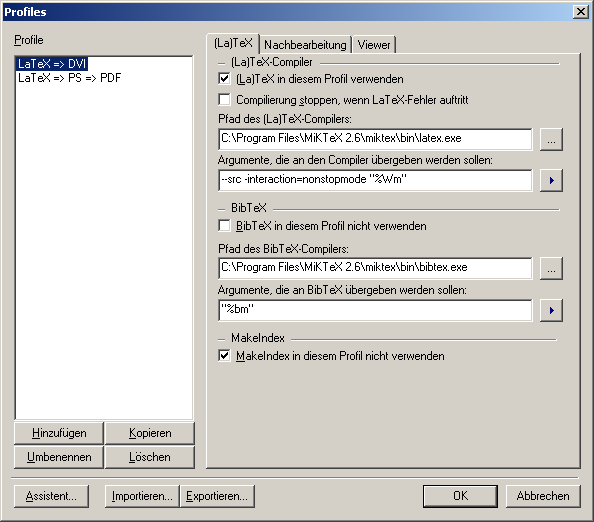
\includegraphics[width=0.49\textwidth]{techniccenter-profile-dvi-26} &
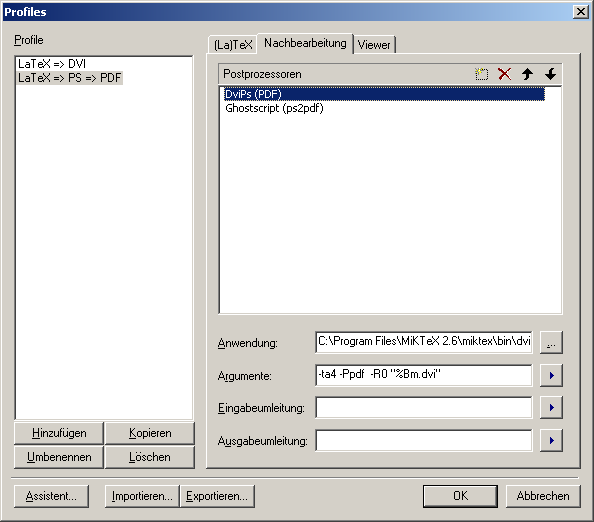
\includegraphics[width=0.49\textwidth]{techniccenter-profile-dvips-26} \\[4pt]
(a) & (b)
\end{tabular}
\caption{Spezifikation der Ausgabeprofile in TeXnicCenter.}
\label{fig:techniccenter-profile-latex}
\end{figure}

Für diese Vorlage wird die verwendung des Ausgabeprofiels \texttt{LaTeX => PDF} empfohlen.

%
%In der Datei \verb!tc_output_profiles_sumatra.tco! sind  folgende beiden "`maßgeschneiderten"' Ausgabeprofile für TexNicCenter angelegt (Import über \textsf{Build} $\rightarrow$ \textsf{Define Output Profiles ...}):
%\begin{itemize}
	%\item \verb!LaTeX => PDF (Sumatra)! -- Standard, direkte Erzeugung von PDF,
	%\item \verb!LaTeX => PS => PDF (Sumatra)! -- PDF "`klassisch"' via DVI und PS.
%\end{itemize}
%
%
%
%\subsubsection{Profil "`\texttt{LaTeX => PDF (Sumatra)}"'}
%
%Das ist das mit diesem Setup normalerweise verwendete Standardprofil.
%
%\paragraph{(La)Tex:}
%\begin{itemize}
  %\item Path to the (La)TeX compiler: \\
        %\begin{small} \verb!C:\Program Files\MiKTeX 2.8\miktex\bin\pdflatex.exe!\end{small}
  %\item Command line arguments to pass to the compiler:\\
%\begin{small}
   %\verb!-synctex=-1 -interaction=nonstopmode "%pm"!
%\end{small}
%\end{itemize}
%
%\paragraph{Postprocessor:} 
%leer, kein Postprocessor notwenig.
%
%\paragraph{Viewer:}
%\begin{itemize}
%\item Path of executable: \\
%\begin{small}
    %\verb!C:\Program Files\SumatraPDF\SumatraPDF.exe ! \\ 
    %\verb!-inverse-search "\"C:\Program Files\TeXnicCenter\TEXCNTR.EXE\" !\\
    %\verb!/ddecmd \"[goto('%f','%l')]\""!
%\end{small}
%%
%\item View project's output: \\
%\begin{small}
    %\checkbox\ Command line argument \\\
    %Command: \verb!"%bm.pdf"!
%\end{small}
%%
%\item Forward search:\\
%\begin{small}
    %\checkbox\ DDE command \\\
    %Command: \verb![ForwardSearch("%bm.pdf","%Wc",%l,0)]! \\
    %Server: \verb!SUMATRA! \\
    %Topic: \verb!Control!
%\end{small}
%\item Close document before running (La)TeX:\\
%\begin{small}
    %\checkbox\ Do not close
%\end{small}
%\end{itemize}
%
%
%
%
%\subsubsection{Profil "`\texttt{LaTeX => PS => PDF (Sumatra)}"'}
%
%Profil ausschließlich für den DVI-PS-Workflow (über DVI und PostScript).
%
%\paragraph{(La)Tex:}
%\begin{itemize}
  %\item Path to the (La)TeX compiler: \\
        %\begin{small} \verb!C:\Program Files\MiKTeX 2.8\miktex\bin\latex.exe!\end{small}
  %\item Command line arguments to pass to the compiler:\\
%\begin{small}
   %\verb!-synctex=-1 -interaction=nonstopmode "%pm"!
%\end{small}
%\end{itemize}
%
%\paragraph{Postprocessor:}
%\begin{itemize}
  %\item DviPS (PDF): \\
        %\begin{small} 
        %Executable: \verb!C:\Program Files\MiKTeX 2.8\miktex\bin\dvips.exe! \\
        %Arguments: \verb!-ta4 -P pdf -R0 "%Bm.dvi"!
        %\end{small}
  %\item Ghostscript (ps2pdf):\\
  		%\begin{small} 
        %Executable: \verb!C:\Program Files\gs\gs8.64\bin\gswin32c.exe! \\
        %Arguments: \verb!-q -dPDFSETTINGS=/prepress -sPAPERSIZE=a4 -dSAFER! \\
         %\verb!-dBATCH -dNOPAUSE -sDEVICE=pdfwrite -sOutputFile="%bm.pdf"! \\
         %\verb!-c save pop -f "%bm.ps"!
      %\end{small}
%\end{itemize}
%
%\paragraph{Viewer:}
%wie in Profil A. (\texttt{LaTeX => PDF (Sumatra)}).
	% Technische Ergänzungen
\chapter{Inhalt der CD-ROM/DVD}
\label{app:cdrom}

\paragraph{Format:} 
		CD-ROM, Single Layer, ISO9660-Format%
\footnote{Verwenden Sie möglichst ein Standardformat, bei DVDs natürlich
eine entsprechende andere Spezifikation.}


\section{PDF-Dateien}
\begin{FileList}{/}
\fitem{_Diplomarbeit.pdf} Diplomarbeit mit Instruktionen (Gesamtdokument)
%
\end{FileList}


\section{\latex-Dateien}

\textbf{Achtung:} Die folgende Auflistung soll nur den Gebrauch dieser Vorlage
erleichtern. Es ist bei einer Diplomarbeit \ia\ \emph{nicht} notwendig, die zugehörigen \latex-Dateien aufzulisten (wohl aber projektbezogene Dateien, Ergebnisse, Bilder, Kopien von Online-Literatur etc.)!
%\paragraph{Pfad:} \url{/}
\begin{FileList}{/}
\fitem{_Diplomarbeit.tex} Diplomarbeit (Hauptdokument) %
\fitem{vorwort.tex} Vorwort %
\fitem{kurzfassung.tex} Kurzfassung %
\fitem{abstract.tex} Abstract %
\fitem{einleitung.tex} Kapitel 1 %
\fitem{diplomschrift.tex} Kapitel 2 %
\fitem{latex.tex} Kapitel 3
\fitem{abbildungen.tex} Kapitel 4 %
\fitem{formeln.tex} Kapitel 5 %
\fitem{literatur.tex} Kapitel 6 %
\fitem{drucken.tex} Kapitel 7 %
\fitem{word.tex} Kapitel 8 %
\fitem{schluss.tex} Kapitel 9 %
\fitem{anhang_a.tex} Anhang A (Source Code) %
\fitem{anhang_b.tex} Anhang B (Inhalt CD-ROM) %
\fitem{anhang_c.tex} Anhang C (Änderungen) %
\fitem{anhang_d.tex} Anhang D (Latex Quellcode) %
\fitem{messbox.tex} Messbox zur Druckkontrolle %
\fitem{literatur.bib} Literatur-Datenbank (BibTeX-File)
\end{FileList}

\begin{comment}
\section{Dokumentation}
%\paragraph{Pfad:} \url{/docs/}
\begin{FileList}{/docs/}
\fitem{caption2.pdf}  \texttt{caption} Paket %
\fitem{fancyhdr.pdf} "`Fancy Headers"' Paket %
\fitem{float.pdf}     \texttt{float}
Paket \fitem{gerdoc.pdf}    Kurzbeschreibung zu \texttt{german.sty}
und \texttt{ngerman.sty} \fitem{grfguide.pdf}  \texttt{graphicx} Paket
\fitem{l2kurz.pdf}    \latex-Anleitung (deutsch)
\fitem{lshort.pdf}    \latex-Anleitung (englisch)
\fitem{subfigure.pdf} \texttt{subfigure} Paket
\fitem{symbols-a4.pdf} Verzeichnis aller \latex-Symbole
\end{FileList}
\end{comment}

\section{Style/Class-Dateien}
%\paragraph{Pfad:} \url{/}
\begin{FileList}{/}
\fitem{htldipl.sty} Class-File für dieses Dokument
\fitem{htl.sty} Style-File für dieses Dokument
\fitem{algorithmicx.sty}  \texttt{algorithmicx} Paket (Version 1.1) 
\fitem{algpseudocode.sty} \texttt{algpseudocode} Paket 
\fitem{listings2.cfg} \texttt{listings2} Paket 
\fitem{listings2.sty} \texttt{listings2} Paket 
\fitem{lstaspects.sty} \texttt{listings2} Paket 
\fitem{lstdoc2.sty} \texttt{listings2} Paket 
\fitem{lstlanguages.sty} \texttt{listings2} Paket 
\end{FileList}


\section{Sonstiges}
\begin{FileList}{/images}
\fitem{*.ai} Original Adobe Illustrator-Dateien %
\fitem{*.fh11} Original Macromedia Freehand-Dateien %
\fitem{*.jpg} Original Rasterbilder %
\fitem{*.eps} Bilder und Grafiken im EPS-Format%
%\fitem{fonts-bakoma/} BaKoMa TrueType Fonts %
\end{FileList}
	% Inhalt der CD-ROM/DVD
\chapter{Chronologische Liste der Änderungen}

\begin{sloppypar}
\begin{description}

\item[2018/07/02]
Überarbeitung für das Schuljahr 2018/19
\begin{itemize}
  \item Indixierung der Literatur nach Titel und Autor
  \item Allgemeiner Index für eigene Begriffe
  \item Software überarbeitet und auf den neuesten Stand gebracht
  \item Umstieg von biblatex auf biber
  \item Subfigure hinzugefügt
  \item Settings aus \_Diplomarbeit.tex ausgelagert
\end{itemize}


\item[2017/04/03]
FAQ hinzugefügt

\item[2017/03/28]
Anpassungen an sehr lange URLs in den Fußnoten

\item[2017/03/21]
Anpassungen an sehr lange Titel und Untertitel

\item[2016/10/20]
Neues Zitierformat (footcite)

\item[2016/04/04]
Umlaute in Codelistings möglich

\item[2015/10/11]
Dokumentationsseiten aus PDF Formular

\item[2015/10/07]
Umstieg von listings2 auf listingsutf8

\item[2015/10/06]
Syntax Highlighting umschaltbar zwischen Farbe und Schwarz / Weiß

\item[2015/09/29]
Neues Deckblatt

\item[2015/09/03]
Einseitig / Zweiseitig umschaltbar 

\item[2012/08/29]
Einstellbare Seitenränder durch das geometry Package

\item[2010/11/22]
Überarbeitung der originalen Vorlagen von Dr.\ Wilhelm Burger und Anpassung an
die Bedürfnisse einer HTL-
Wichtigste Änderungen:
\begin{itemize}
  \item Wechsel auf UTF8
  \item Wechsel auf listings2-beta
  \item Neue Code-Umgebungen für Python und C\#
  \item Vorlagen für Normen und Patente im Literaturverzeichnis
  \item Hinweise auf DVI-PS Workflow entfernt
  \item Kapitel zur automatischen \latex-Code erzeugung hinzugefügt
\end{itemize}
%
\end{description}

\end{sloppypar}

%\section*{To Do} 
%\begin{itemize}
%\item Literaturempfehlungen zum Schreiben von Diplomarbeiten
%\item Hinweise für Literatursuche (Bibliotheksverbund, CiteSeer,...)
%\end{itemize}



	% Chronologische Liste der Änderungen
\chapter{\latex-Quellkode}
\label{app:latex}

\section*{Hauptdatei {\tt\_Diplomarbeit.tex}}

\begin{footnotesize}
\verbatiminput{_Diplomarbeit.tex}
\end{footnotesize}


%\vspace*{2cm}
\hrule
\hrule

\paragraph{Anmerkung:}
Das sollte nur ein \emph{Beispiel} für die Einbindung von Quellcode
in einem Anhang sein. Der \latex-Quellkode der eigenen
Diplomarbeit ist meist \emph{nicht} interessant genug, um ihn hier
wiederzugeben!

	% Quelltext dieses Dokuments

%%%----------------------------------------------------------
%Ausgabe der automatischen Zusatzdaten: Glossar, Index, Literaturverzeichnis
\clearpage
\printglossaries

\clearpage
\chapter*{Index}
\addcontentsline{toc}{chapter}{Index}
\printindex[allgemein]

\printindex

\printindex[name]

\printindex[title]


%Literaturverzeichnis
\clearpage
\addcontentsline{toc}{chapter}{\bibname}

\printbibliography


%%%----------------------------------------------------------

%%%Messbox zur Druckkontrolle
%\chapter*{Messbox zur Druckkontrolle}



\begin{center}
{\Large --- Druckgröße kontrollieren! ---}

\bigskip

\Messbox{100}{50} % Angabe der Breite/Hoehe in mm

\bigskip

{\Large --- Diese Seite nach dem Druck entfernen! ---}

\end{center}



\end{document}
